\documentclass[a4paper,12pt,twoside]{memoir}

% Castellano
\usepackage[spanish,es-tabla]{babel}
\selectlanguage{spanish}
\usepackage[utf8]{inputenc}
\usepackage[T1]{fontenc}
\usepackage{lmodern} % scalable font
\usepackage{microtype}
\usepackage{placeins}

\RequirePackage{booktabs}
\RequirePackage[table]{xcolor}
\RequirePackage{xtab}
\RequirePackage{multirow}

% Links
\PassOptionsToPackage{hyphens}{url}\usepackage[colorlinks]{hyperref}
\hypersetup{
	allcolors = {red}
}

% Ecuaciones
\usepackage{amsmath}

% Rutas de fichero / paquete
\newcommand{\ruta}[1]{{\sffamily #1}}

% Párrafos
\nonzeroparskip

% Huérfanas y viudas
\widowpenalty100000
\clubpenalty100000

% Evitar solapes en el header
\nouppercaseheads

% Imagenes
\usepackage{graphicx}
\newcommand{\imagen}[2]{
	\begin{figure}[!h]
		\centering
		\includegraphics[width=0.9\textwidth]{#1}
		\caption{#2}\label{fig:#1}
	\end{figure}
	\FloatBarrier
}

\newcommand{\imagenflotante}[2]{
	\begin{figure}%[!h]
		\centering
		\includegraphics[width=0.9\textwidth]{#1}
		\caption{#2}\label{fig:#1}
	\end{figure}
}



% El comando \figura nos permite insertar figuras comodamente, y utilizando
% siempre el mismo formato. Los parametros son:
% 1 -> Porcentaje del ancho de página que ocupará la figura (de 0 a 1)
% 2 --> Fichero de la imagen
% 3 --> Texto a pie de imagen
% 4 --> Etiqueta (label) para referencias
% 5 --> Opciones que queramos pasarle al \includegraphics
% 6 --> Opciones de posicionamiento a pasarle a \begin{figure}
\newcommand{\figuraConPosicion}[6]{%
  \setlength{\anchoFloat}{#1\textwidth}%
  \addtolength{\anchoFloat}{-4\fboxsep}%
  \setlength{\anchoFigura}{\anchoFloat}%
  \begin{figure}[#6]
    \begin{center}%
      \Ovalbox{%
        \begin{minipage}{\anchoFloat}%
          \begin{center}%
            \includegraphics[width=\anchoFigura,#5]{#2}%
            \caption{#3}%
            \label{#4}%
          \end{center}%
        \end{minipage}
      }%
    \end{center}%
  \end{figure}%
}

%
% Comando para incluir imágenes en formato apaisado (sin marco).
\newcommand{\figuraApaisadaSinMarco}[5]{%
  \begin{figure}%
    \begin{center}%
    \includegraphics[angle=90,height=#1\textheight,#5]{#2}%
    \caption{#3}%
    \label{#4}%
    \end{center}%
  \end{figure}%
}
% Para las tablas
\newcommand{\otoprule}{\midrule [\heavyrulewidth]}
%
% Nuevo comando para tablas pequeñas (menos de una página).
\newcommand{\tablaSmall}[5]{%
 \begin{table}
  \begin{center}
   \rowcolors {2}{gray!35}{}
   \begin{tabular}{#2}
    \toprule
    #4
    \otoprule
    #5
    \bottomrule
   \end{tabular}
   \caption{#1}
   \label{tabla:#3}
  \end{center}
 \end{table}
}

%
%Para el float H de tablaSmallSinColores
\usepackage{float}

%
% Nuevo comando para tablas pequeñas (menos de una página).
\newcommand{\tablaSmallSinColores}[5]{%
 \begin{table}[H]
  \begin{center}
   \begin{tabular}{#2}
    \toprule
    #4
    \otoprule
    #5
    \bottomrule
   \end{tabular}
   \caption{#1}
   \label{tabla:#3}
  \end{center}
 \end{table}
}

\newcommand{\tablaApaisadaSmall}[5]{%
\begin{landscape}
  \begin{table}
   \begin{center}
    \rowcolors {2}{gray!35}{}
    \begin{tabular}{#2}
     \toprule
     #4
     \otoprule
     #5
     \bottomrule
    \end{tabular}
    \caption{#1}
    \label{tabla:#3}
   \end{center}
  \end{table}
\end{landscape}
}

%
% Nuevo comando para tablas grandes con cabecera y filas alternas coloreadas en gris.
\newcommand{\tabla}[6]{%
  \begin{center}
    \tablefirsthead{
      \toprule
      #5
      \otoprule
    }
    \tablehead{
      \multicolumn{#3}{l}{\small\sl continúa desde la página anterior}\\
      \toprule
      #5
      \otoprule
    }
    \tabletail{
      \hline
      \multicolumn{#3}{r}{\small\sl continúa en la página siguiente}\\
    }
    \tablelasttail{
      \hline
    }
    \bottomcaption{#1}
    \rowcolors {2}{gray!35}{}
    \begin{xtabular}{#2}
      #6
      \bottomrule
    \end{xtabular}
    \label{tabla:#4}
  \end{center}
}

%
% Nuevo comando para tablas grandes con cabecera.
\newcommand{\tablaSinColores}[6]{%
  \begin{center}
    \tablefirsthead{
      \toprule
      #5
      \otoprule
    }
    \tablehead{
      \multicolumn{#3}{l}{\small\sl continúa desde la página anterior}\\
      \toprule
      #5
      \otoprule
    }
    \tabletail{
      \hline
      \multicolumn{#3}{r}{\small\sl continúa en la página siguiente}\\
    }
    \tablelasttail{
      \hline
    }
    \bottomcaption{#1}
    \begin{xtabular}{#2}
      #6
      \bottomrule
    \end{xtabular}
    \label{tabla:#4}
  \end{center}
}

%
% Nuevo comando para tablas grandes sin cabecera.
\newcommand{\tablaSinCabecera}[5]{%
  \begin{center}
    \tablefirsthead{
      \toprule
    }
    \tablehead{
      \multicolumn{#3}{l}{\small\sl continúa desde la página anterior}\\
      \hline
    }
    \tabletail{
      \hline
      \multicolumn{#3}{r}{\small\sl continúa en la página siguiente}\\
    }
    \tablelasttail{
      \hline
    }
    \bottomcaption{#1}
  \begin{xtabular}{#2}
    #5
   \bottomrule
  \end{xtabular}
  \label{tabla:#4}
  \end{center}
}

\usepackage{lscape}

\definecolor{cgoLight}{HTML}{EEEEEE}
\definecolor{cgoExtralight}{HTML}{FFFFFF}

%
% Nuevo comando para tablas grandes sin cabecera.
\newcommand{\tablaSinCabeceraConBandas}[5]{%
  \begin{center}
    \tablefirsthead{
      \toprule
    }
    \tablehead{
      \multicolumn{#3}{l}{\small\sl continúa desde la página anterior}\\
      \hline
    }
    \tabletail{
      \hline
      \multicolumn{#3}{r}{\small\sl continúa en la página siguiente}\\
    }
    \tablelasttail{
      \hline
    }
    \bottomcaption{#1}
    \rowcolors[]{1}{cgoExtralight}{cgoLight}

  \begin{xtabular}{#2}
    #5
   \bottomrule
  \end{xtabular}
  \label{tabla:#4}
  \end{center}
}




\graphicspath{ {./img/} }

% Capítulos
\chapterstyle{bianchi}
\newcommand{\capitulo}[2]{
	\setcounter{chapter}{#1}
	\setcounter{section}{0}
	\setcounter{figure}{0}
	\setcounter{table}{0}
	\chapter*{#2}
	\addcontentsline{toc}{chapter}{#2}
	\markboth{#2}{#2}
}

% Apéndices
\renewcommand{\appendixname}{Apéndice}
\renewcommand*\cftappendixname{\appendixname}

\newcommand{\apendice}[1]{
	%\renewcommand{\thechapter}{A}
	\chapter{#1}
}

\renewcommand*\cftappendixname{\appendixname\ }

% Formato de portada
\makeatletter
\usepackage{xcolor}
\newcommand{\tutor}[1]{\def\@tutor{#1}}
\newcommand{\course}[1]{\def\@course{#1}}
\definecolor{cpardoBox}{HTML}{E6E6FF}
\def\maketitle{
  \null
  \thispagestyle{empty}
  % Cabecera ----------------
\noindent
\includegraphics[width=\textwidth]{cabecera}\vspace{1cm}%
  \vfill
  % Título proyecto y escudo informática ----------------
  \colorbox{cpardoBox}{%
    \begin{minipage}{.8\textwidth}
      \vspace{.5cm}\Large
      \begin{center}
      \textbf{TFG del Grado en Ingeniería Informática}\vspace{.6cm}\\
      \textbf{\LARGE\@title{}}
      \end{center}
      \vspace{.2cm}
    \end{minipage}

  }%
  \hfill\begin{minipage}{.20\textwidth}
    
\includegraphics[width=\textwidth]{escudoInfor}
  \end{minipage}
  \vfill
  % Datos de alumno, curso y tutores ------------------
  \begin{center}%
  {%
    \noindent\LARGE
    Presentado por \@author{}\\ 
    en Universidad de Burgos  \\ \@date{}\\
    Tutor: \@tutor{}\\
  }%
  \end{center}%
  \null
  \cleardoublepage
  }
\makeatother


% Datos de portada
\title{XacoMeter II \\Documentación Técnica}
\author{Natalia Franco}
\tutor{Jose Ignacio Santos Martín, Virginia Ahedo García  y Silvia Díaz de la Fuente}
\date{\today}

\begin{document}

\maketitle



\cleardoublepage



%%%%%%%%%%%%%%%%%%%%%%%%%%%%%%%%%%%%%%%%%%%%%%%%%%%%%%%%%%%%%%%%%%%%%%%%%%%%%%%%%%%%%%%%



\frontmatter


\clearpage

% Indices
\tableofcontents

\clearpage

\listoffigures

\clearpage

\listoftables

\clearpage

\mainmatter

\appendix

\apendice{Plan de Proyecto Software}

\section{Introducción}
La primera fase de un proyecto es la planificación del mismo, la fase más importante para poder estimar el trabajo, el tiempo y el dinero que va a suponer su realización. En este anexo podremos ver detalladamente cada una de las estimaciones realizadas para valorar más tarde el desarrollo y los costes que verdaderamente han sido producidos.
La planificación del proyecto a su vez, se desglosa en dos estudios:
\begin{itemize}
    \item {La planificación temporal}
    \item {El estudio de viabilidad económica y legal}
\end{itemize}



\section{Planificación temporal}
La planificación temporal se ha llevado a cabo a través de un repositorio específico en Github llamado XacoMeterII-Twitter con url: \url{https://github.com/nataliafraanco/XacoMeterII-Twitter}\\
Para relizar el control del proyecto se ha utilizado la herramienta Zenhub de Github. Con ésta, se ha dividido el proyecto en \textit{sprints}, con una duración cada uno de dos semanas, que a su vez se dividen en diferentes tareas a resolver.\\
La visualización de las tareas realizadas en cada sprint y su resolución se ha llevado a cabo a través de \textit{"Burndown reports"}, los cuales consisten en mostrar gráficamente la evolución del proyecto en cada uno de los \textit{sprints}.

\subsection{Sprint 0 : 28 Septiembre 2022 - 13 Octubre 2022}
El primer \textit{sprint} fue una toma de contacto con el trabajo. Entender qué es lo que quería hacer y qué necesitaba para ello, es decir, investigar sobre cada una de las herramientas necesarias y decidir cuáles iba a implementar, antes comparando todas las opciones.
Además se montó un inicio de lo que podría ser el origen de la página web, aunque al ser solo un boceto se modificaría en otros \textit{sprints} más adelante.
Además, en un primer momento me propuse empezar a trabajar con la API de Twitter, pero no contabilicé bien los tiempos e invertí todo mi tiempo en la búsqueda de la información necesaria para comenzar, por lo que los anteriores issues decidí realizarlos en el siguiente \textit{sprint}.
En el siguiente gráfico que se muestra a continuación, se puede ver mi evolución dentro del \textit{sprint}.
\imagen{Sprint0}{Sprint 0 - Gráfica informe de evolución}


\tablaSmallSinColores{Sprint 0 - Tabla de tareas y tiempos}{p{5cm} p{4cm} p{4cm}}{Sprint 0 - Tabla de tareas y tiempos}
{
  \multicolumn{1}{p{5cm}}{\textbf{Tareas realizadas}} & \textbf{Tiempo estimado (h)} & \textbf{{Tiempo empleado (h)}}\\
 }
 {
Investigación sobre herramientas  & \multicolumn{1}{r}{10}& \multicolumn{1}{r}{15}\\
Elección de herramientas  & \multicolumn{1}{r}{3}& \multicolumn{1}{r}{3}\\
Inciciación con LateX  & \multicolumn{1}{r}{3}& \multicolumn{1}{r}{2}\\
Esquema página web  & \multicolumn{1}{r}{8}& \multicolumn{1}{r}{5}\\
Implementar API Twitter  & \multicolumn{1}{r}{5}& \multicolumn{1}{r}{-}\\\hline
\textbf{Tiempos totales}  & \multicolumn{1}{r}{29} & \multicolumn{1}{r}{25}\\
}


\subsection{Sprint 1 : 13 Octubre 2022 - 26 Octubre 2022}
En este \textit{sprint} he completado las tareas que no completé en el \textit{sprint} 0.
Implementé una manera de utilizar la API de Twitter para poder abstraer los datos, y en un principio lo desarrollé mediante la herramienta \textit{Tweepy} y con unos permisos esenciales.
La tutora consiguió obtener los permisos necesarios para tener una cuenta educativa con sus datos, pero a la hora de introducir las credenciales causaba varios fallos, los cuales me llevaron bastante tiempo arreglar y no llegué a tiempo para terminarlos en este \textit{sprint}, por lo que se terminó en el siguiente.
\imagen{Sprint1}{Sprint 1 - Gráfica informe de evolución}

\tablaSmallSinColores{Sprint 1 - Tabla de tareas y tiempos}{p{5cm} p{4cm} p{4cm}}{Sprint 1 - Tabla de tareas y tiempos}
{
  \multicolumn{1}{p{5cm}}{\textbf{Tareas realizadas}} & \textbf{Tiempo estimado (h)} & \textbf{{Tiempo empleado (h)}}\\
 }
 {
Implementar API Twitter(Sprint 0)  & \multicolumn{1}{r}{5}& \multicolumn{1}{r}{30}\\
Acceder con credenciales educativas  & \multicolumn{1}{r}{21}& \multicolumn{1}{r}{20}\\
Selección de campos a obtener  & \multicolumn{1}{r}{2}& \multicolumn{1}{r}{-}\\\hline
\textbf{Tiempos totales}  & \multicolumn{1}{r}{28} & \multicolumn{1}{r}{50}\\
}


\subsection{Sprint 2 : 26 Octubre 2022 - 9 Noviembre 2022}
En el este tercer \textit{sprint}, se continuó intentando introducir las credenciales educativas. Tras varias reuniones con los tutores, encontramos el fallo y conseguimos continuar. Se aplicaron los cambios, se decidieron los parámetros que se iban a utilizar y cómo incluirlos para obtener los resultados esperados de la API de Twitter para un futuro uso en la aplicación.
En este \textit{sprint} se intentó avanzar lo que llevaba atrasado debido a la parada que me causó el fallo con las credenciales educativas y decidí crear la base de datos.\\
Además, se creó una nube de palabras con los datos obtenidos de la API para poder tener algo visual y ver que funcionaba todo correctamente, aunque aún no se había decidido si esa nube de palabras constaría en el proyecto final.\\
Se comenzó también a implementar varias funciones que insertasen los datos obtenidos en la base de datos. Al ser mucho trabajo para este \textit{sprint}, continué con estas tareas en los siguientes \textit{sprints}.
\imagen{Sprint2}{Sprint 2 - Gráfica informe de evolución}
\tablaSmallSinColores{Sprint 2 - Tabla de tareas y tiempos}{p{5cm} p{4cm} p{4cm}}{Sprint 2 - Tabla de tareas y tiempos}
{
  \multicolumn{1}{p{5cm}}{\textbf{Tareas realizadas}} & \textbf{Tiempo estimado (h)} & \textbf{{Tiempo empleado (h)}}\\
 }
 {
Acceder con credenciales educativas (Sprint 1)  & \multicolumn{1}{r}{40}& \multicolumn{1}{r}{15}\\
Selección de campos a obtener (Sprint 1)  & \multicolumn{1}{r}{2}& \multicolumn{1}{r}{2}\\
Elección de base de datos y creación  & \multicolumn{1}{r}{13}& \multicolumn{1}{r}{25}\\
Gráfico con nube de palabras  & \multicolumn{1}{r}{3}& \multicolumn{1}{r}{5}\\
Verificación de filtros API Twitter  & \multicolumn{1}{r}{3}& \multicolumn{1}{r}{4}\\
Insertar datos en la base de datos  & \multicolumn{1}{r}{8}& \multicolumn{1}{r}{15}\\\hline
\textbf{Tiempos totales}  & \multicolumn{1}{r}{69} & \multicolumn{1}{r}{66}\\
}

\subsection{Sprint 3 : 9 Noviembre 2022 - 23 Noviembre 2022}
Este \textit{sprint} se dedicó totalmente a la inserción de datos en la base de datos. 
Se consiguió que la aplicación, una vez ejecutada, accediera a los datos mediante la API y los insertara correctamente en las dos tablas de las que consta la base de datos.
\imagen{Sprint3}{Sprint 3 - Gráfica informe de evolución}

\tablaSmallSinColores{Sprint 3 - Tabla de tareas y tiempos}{p{5cm} p{4cm} p{4cm}}{Sprint 3 - Tabla de tareas y tiempos}
{
  \multicolumn{1}{p{5cm}}{\textbf{Tareas realizadas}} & \textbf{Tiempo estimado (h)} & \textbf{{Tiempo empleado (h)}}\\
 }
 {
Insertar datos en base de datos (Sprint 2)  & \multicolumn{1}{r}{8}& \multicolumn{1}{r}{35}\\
Redacción de documentación en LateX  & \multicolumn{1}{r}{40}& \multicolumn{1}{r}{10}\\\hline
\textbf{Tiempos totales}  & \multicolumn{1}{r}{48} & \multicolumn{1}{r}{45}\\
}


\subsection{Sprint 4 : 23 Noviembre 2022 - 7 Diciembre 2022}
Llegados a este momento del proyecto, se decidió crear una interfaz gráfica más avanzada. Se decidió que hubiese un administrador que sea el que se encargue de acceder a la API de twitter y decida si quiere crear una base de datos desde una fecha o si actualizar la base de datos ya creada. \\
Por otro lado, los usuarios solo van a tener la opción de entrar en la aplicación y visualizar mediante gráficos estadísticos los datos almacenados.
Esto se decidió de esta manera para no alargar el tiempo de espera del usuario al tener que obtener los datos, debido a que hay unas limitaciones de poder realizar solo 300 consultas cada 15 minutos.
Se continúa realizando también la documentación en \LaTeX.
\imagen{Sprint4}{Sprint 4 - Gráfica informe de evolución}
\tablaSmallSinColores{Sprint 4 - Tabla de tareas y tiempos}{p{5cm} p{4cm} p{4cm}}{Sprint 4 - Tabla de tareas y tiempos}
{
  \multicolumn{1}{p{5cm}}{\textbf{Tareas realizadas}} & \textbf{Tiempo estimado (h)} & \textbf{Tiempo empleado (h)}\\
 }
 {
Montar inicio de la aplicación  & \multicolumn{1}{r}{8}& \multicolumn{1}{r}{15}\\
redacción en LateX  & \multicolumn{1}{r}{40}& \multicolumn{1}{r}{15}\\
Diseñar usuario administrador  & \multicolumn{1}{r}{13}& \multicolumn{1}{r}{15}\\\hline
\textbf{Tiempos totales}  & \multicolumn{1}{r}{61} & \multicolumn{1}{r}{45}\\
}


\subsection{Sprint 5 : 7 Diciembre 2022 - 21 Diciembre 2022}
En este \textit{sprint} se decidió desarrollar la parte gráfica del inicio y mejorar las pestañas del administrador, además de proteger las vistas que solo el administrador puede manejar, denegando el acceso a los usuarios no identificados.\\
También se decidió mejorar la base de datos, creando un nuevo parámetro que almacene un booleano \textit{'True'} o \textit{'False'} referido a si el \textit{tweet} de cada BIC estaba borrado o no, todo ello manejado con la opción de crear base de datos. Este parámetro se incluye para ahorrar peticiones a la API de twitter y para poder reutilizar datos anteriormente recuperados, de esta manera también se mejora mucho el rendimiento de la aplicación.
\imagen{Sprint5}{Sprint 5 - Gráfica informe de evolución}
\tablaSmallSinColores{Sprint 5 - Tabla de tareas y tiempos}{p{5cm} p{4cm} p{4cm}}{Sprint 5 - Tabla de tareas y tiempos}
{
  \multicolumn{1}{p{5cm}}{\textbf{Tareas realizadas}} & \textbf{Tiempo estimado (h)} & \textbf{Tiempo empleado (h)}\\
 }
 {
Creación de Administrador  & \multicolumn{1}{r}{13}& \multicolumn{1}{r}{15}\\
Creación de base de datos desde el administrador pasando fecha inicio  & \multicolumn{1}{r}{8}& \multicolumn{1}{r}{8}\\
Creación parte gráfica del inicio
  & \multicolumn{1}{r}{13}& \multicolumn{1}{r}{15}\\
Crear diseño gráfico de Login (administrador)  & \multicolumn{1}{r}{8}& \multicolumn{1}{r}{7}\\
Añadir parámetro “Borrado” para gestión de base de datos
  & \multicolumn{1}{r}{5}& \multicolumn{1}{r}{3}\\
Cambiar comportamiento de la base de datos
  & \multicolumn{1}{r}{13}& \multicolumn{1}{r}{8}\\
Protección de vistas del Administrador
 & \multicolumn{1}{r}{13}& \multicolumn{1}{r}{15}\\\hline
\textbf{Tiempos totales}  & \multicolumn{1}{r}{73} & \multicolumn{1}{r}{71}\\
}

\subsection{Sprint 6 : 21 Diciembre 2022 - 4 Enero 2023}
Una vez montada la interfaz gráfica para la parte del administrador, se decidió montar el inicio para todos los usuarios, queriendo mostrar con originalidad los \textit{BICs} (Bienes de Interes Cultural). Se decidió integrar un mapa para que los usuarios pudiesen situar el \textit{BIC} en un mapa.\\
Una vez hecho el mapa se colocaron los \textit{BICs} geolocalizados, de tal manera que al hacer click sobre cada uno de ellos, se redirecciona al usuario a una página de estadísticas del mismo patrimonio.\\
También plantea la posibilidad de crear una página de estadísticas con un gráfico temporal para ir viendo el funcionamiento y comprobar que la extracción de información de la base de datos y el redireccionamiento funcionan correctamente.
\imagen{Sprint6}{Sprint 6 - Gráfica informe de evolución}
\tablaSmallSinColores{Sprint 6 - Tabla de tareas y tiempos}{p{5cm} p{4cm} p{4cm}}{Sprint 6 - Tabla de tareas y tiempos}
{
  \multicolumn{1}{p{5cm}}{\textbf{Tareas realizadas}} & \textbf{Tiempo estimado (h)} & \textbf{Tiempo empleado (h)}\\
 }
 {
Crear mapa didáctico en inicio  & \multicolumn{1}{r}{13}& \multicolumn{1}{r}{15}\\
Implementar API para mapas (decidir entre leaflet y google maps)  & \multicolumn{1}{r}{13}& \multicolumn{1}{r}{20}\\
Crear página de estadisticas con un gráfico de series temporales  & \multicolumn{1}{r}{8}& \multicolumn{1}{r}{15}\\
Búsqueda en la base de datos los datos del patrimonio elegido y contar numero de tweets  & \multicolumn{1}{r}{5}& \multicolumn{1}{r}{7}\\
Redireccionar iconos del mapa a página de estadisticas  & \multicolumn{1}{r}{8}& \multicolumn{1}{r}{15}\\\hline
\textbf{Tiempos totales}  & \multicolumn{1}{r}{47} & \multicolumn{1}{r}{72}\\
}


\subsection{Sprint 7 : 4 Enero 2023 - 18 Enero 2023}
En este \textit{sprint}, se quiso cambiar la barra superior de navegación a una barra lateral, ya esto aportará una mayor visibilidad del mapa de las localidades.\\
También se decidió ampliar la página de estadísticas para albergar tres gráficos que visualicen varios datos importantes de cada \textit{BIC}, así como sus métricas públicas y la comparación de tweets respecto a otros \textit{BICs} entre las mismas fechas.\\
Una parte importante que no se había tenido en cuenta fue el control de excepciones, por lo que en este \textit{sprint} también se decidió implementarlas de tal manera que en el caso de causar alguna excepción, apareciese un mensaje en la aplicación evitando que deje de funcionar y se registre dicho error en un fichero de logs en local.\\
Para que cualquier persona pueda hacer uso de la aplicación se requiere que esta esté desplegada con un dominio, por lo que se desplegará en Heroku con la url \url{https://tfg-nataliafranco-xacometer2.herokuapp.com/}.
Antes de esto, se necesitan crear varios ficheros para su correcto funcionamiento, por ejemplo, Procfile y requirements.txt.
\imagen{Sprint7}{Sprint 7 - Gráfica informe de evolución}
\tablaSmallSinColores{Sprint 7 - Tabla de tareas y tiempos}{p{5cm} p{4cm} p{4cm}}{Sprint 7 - Tabla de tareas y tiempos}
{
  \multicolumn{1}{p{5cm}}{\textbf{Tareas realizadas}} & \textbf{Tiempo estimado (h)} & \textbf{Tiempo empleado (h)}\\
 }
 {
Crear gráfico temporal de tweets  & \multicolumn{1}{r}{8}& \multicolumn{1}{r}{8}\\
Crear gráfico circular de porcentajes  & \multicolumn{1}{r}{8}& \multicolumn{1}{r}{8}\\
Crear gráfico de métricas públicas  & \multicolumn{1}{r}{8}& \multicolumn{1}{r}{8}\\
Controlar excepciones y errores  & \multicolumn{1}{r}{21}& \multicolumn{1}{r}{25}\\
Creación de fichero requirements.txt  & \multicolumn{1}{r}{1}& \multicolumn{1}{r}{1}\\
Creación de fichero Procfile  & \multicolumn{1}{r}{1}& \multicolumn{1}{r}{1}\\
Cambio de barra superior a lateral  & \multicolumn{1}{r}{13}& \multicolumn{1}{r}{15}\\\hline
\textbf{Tiempos totales}  & \multicolumn{1}{r}{60} & \multicolumn{1}{r}{66}\\
}

\subsection{Sprint 8 : 18 Enero 2023 - 1 Febrero 2023}
Una vez creados los ficheros requeridos por Heroku, se procedió al despliegue. En este \textit{sprint} se quiso realizar el despliegue y comprobar el total funcionamiento de la aplicación, perfeccionando las operaciones que causaran fallos.\\
Además, se quiso mejorar la página de estadísticas temporales añadiendo funcionalidades nuevas como son, por un lado, la descarga de los datos en bruto en formato csv para su posible importación en Excel; y por otro lado, la mejora los gráficos para que resultaran más dinámicos y mostrasen más información.
\imagen{Sprint8}{Sprint 8 - Gráfica informe de evolución}
\tablaSmallSinColores{Sprint 8 - Tabla de tareas y tiempos}{p{5cm} p{4cm} p{4cm}}{Sprint 8 - Tabla de tareas y tiempos}
{
  \multicolumn{1}{p{5cm}}{\textbf{Tareas realizadas}} & \textbf{Tiempo estimado (h)} & \textbf{Tiempo empleado (h)}\\
 }
 {
Despliegue en Heroku  & \multicolumn{1}{r}{13}& \multicolumn{1}{r}{10}\\
Cambiar direcciones para utilizar en Heroku  & \multicolumn{1}{r}{3}& \multicolumn{1}{r}{3}\\
Arreglar botones que no redireccionan  & \multicolumn{1}{r}{3}& \multicolumn{1}{r}{5}\\
Crear desplegable de búsqueda  & \multicolumn{1}{r}{8}& \multicolumn{1}{r}{10}\\
Cambiar consulta SQL de estadísticas  & \multicolumn{1}{r}{5}& \multicolumn{1}{r}{4}\\
Cambiar gráficos de matplotlib a plotly  & \multicolumn{1}{r}{5}& \multicolumn{1}{r}{8}\\
Poner título de página de estadísticas  & \multicolumn{1}{r}{2}& \multicolumn{1}{r}{1}\\
Crear botón de descarga de csv  & \multicolumn{1}{r}{2}& \multicolumn{1}{r}{5}\\
Cambiar formato de fechas  & \multicolumn{1}{r}{1}& \multicolumn{1}{r}{1}\\\hline
\textbf{Tiempos totales}  & \multicolumn{1}{r}{42} & \multicolumn{1}{r}{47}\\
}
\subsection{Sprint 9 : 1 Febrero 2023 - 15 Febrero 2023}
Este \textit{sprint}, ya que es el último y la aplicación cumple con todos los objetivos marcados en un inicio, se dedica a terminar de redactar la memoria y los anexos, y añadir nuevas funcionalidades al proyecto. En la última reunión se marcaron los últimos objetivos posibles a realizar que fueron:
\begin{itemize}
    \item Poner la funcionalidad de buscador a la barra desplegable.
    \item Crear la máquina virtual para poder ejecutar el proyecto en local y así utilizar la función de administrador.
    \item Crear una nueva página de estadísticas globales comparando los tweets de todos los BICs entre las fechas que el usuario indique.
    \item Adaptar la apliación a diferentes tamaños de pantalla.
    \item Mostrar mensajes de errores en la aplicación.
    \item Realizar un análisis de sentimientos.
\end{itemize}
Finalmente, se consiguió implementar todos los cambios, incluso el análisis de sentimientos.

\imagen{Sprint9}{Sprint 9 - Gráfica informe de evolución}
\tablaSmallSinColores{Sprint 9 - Tabla de tareas y tiempos}{p{5cm} p{4cm} p{4cm}}{Sprint 9 - Tabla de tareas y tiempos}
{
  \multicolumn{1}{p{5cm}}{\textbf{Tareas realizadas}} & \textbf{Tiempo estimado (h)} & \textbf{Tiempo empleado (h)}\\
 }
 {
Redacción de documentación \LaTeX  & \multicolumn{1}{r}{40}& \multicolumn{1}{r}{50}\\
Funcionalidad de buscador en el desplegable  & \multicolumn{1}{r}{2}& \multicolumn{1}{r}{3}\\
Crear máquina virtual  & \multicolumn{1}{r}{21}& \multicolumn{1}{r}{18}\\
Crear página de estadísticas globales  & \multicolumn{1}{r}{8}& \multicolumn{1}{r}{5}\\
Adaptación a pantallas  & \multicolumn{1}{r}{5}& \multicolumn{1}{r}{8}\\
Mostrar mensajes  & \multicolumn{1}{r}{5}& \multicolumn{1}{r}{5}\\
Sentiment Analysis  & \multicolumn{1}{r}{13}& \multicolumn{1}{r}{10}\\\hline
\textbf{Tiempos totales}  & \multicolumn{1}{r}{94} & \multicolumn{1}{r}{99}\\
}


\subsection{Etiquetas utilizadas}
Para el control de las tareas, se han utilizado etiquetas que definen el tipo de cada una de ellas, para así poder llevar una mejor organización de las mismas.\\
En este proyecto se han hecho uso de las siguientes etiquetas:
\imagen{Etiquetas}{Planificación temporal - Etiquetas}

\section{Estudio de viabilidad}
Además de la planificación temporal, se debe analizar la viabilidad del proyecto desde un punto de vista económico y legal, asumiendo el supuesto desarrollo en el mercado real. 

\subsection{Viabilidad económica}
 A la hora de analizar el proyecto desde un punto de vista económico, se deben tener en cuenta las horas que ha supuesto el desarrollo del proyecto, para así proceder a estimar los costes y beneficios que se producirán en el caso de que una empresa real decidiese llevarlo a cabo.\\
 Para ello, se hace imprescincible tener en cuenta los costes de personal, los cuales van a ser analizados desde dos perspectivas y teniendo en cuenta que el proyecto ha sido realizado por un alumno a tiempo completo durante aproximadamente cinco meses.

\subsubsection{SUELDOS, COSTES SOCIALES Y DE FACTURACIÓN}

En el análisis de este apartado se tendrán en cuenta los siguientes costes:

\begin{itemize}
    \item\textit{} {COSTES DEL TRABAJADOR}

    El trabajador, en este caso el alumno, debe ser contratado de forma directa mediante un contrato de trabajo temporal por circunstancias de la producción, ya que el contrato por obra o servicio desapareció en la última reforma laboral. A este trabajador se le debería aplicar el XVII convenio colectivo estatal de empresas de consultoría y estudios de mercado y de la opinión pública, publicado en el Boletin Oficial del Estado (BOE) el 6 de Marzo de 2018 \cite{BOE}.

    Se calcula que el \textbf{alumno} ha realizado el proyecto en 660 horas totales durante aproximadamente 5 meses, lo que supone que se han dedicado entre 30 y 35 horas semanales, dependiendo de la carga de trabajo.
    Se estima que el sueldo del alumno va a ser de 15€/hora, por lo que se calcula el salario mensual bruto de la siguiente manera:
    $$ 4\frac{\text{semanas}}{\text{meses}}\times32.5\frac{\text{horas}}{\text{semana}}\times15\frac{\text{€}}{\text{hora}}=1950\text{€}\hspace{0.5em}al\hspace{0.5em}mes $$

    Este cálculo corresponde al salario bruto del empleado. se debe tener en cuenta las cotizaciones sociales que debe abonar la , establecidas cada año en el régimen general de la seguridad social. Se pueden consultar estos impuestos en la página oficial de la Seguridad Social \cite{SeguridadSocial}.

    \begin{enumerate}
        \item\textit {Contingencias comunes:}\\
        Porcentaje que paga la empresa por enfermedad común del trabajador.

        \begin{figure}[ht]
              \begin{minipage}{1.3\textwidth}
                \centering
                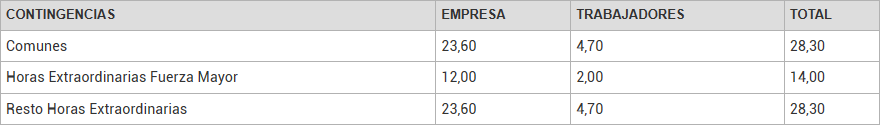
\includegraphics[scale=0.4]{img/Contingencias.png} \\
                \caption{Costes de la empresa - Contingencias comunes}
                \label{Costes de la empresa - Contingencias comunes}
            \end{minipage}
        \end{figure}
        
        \item\textit {Contingencias profesionales y conceptos de recaudación conjunta:}\\
        \begin{enumerate}
            \item\textit {Accidentes de Trabajo (AT):}\\
            Porcentaje que paga la empresa por accidentes de trabajo y enfermedad profesional.\\
            \begin{figure}[h]
              \begin{minipage}{1.3\textwidth}
                \centering
                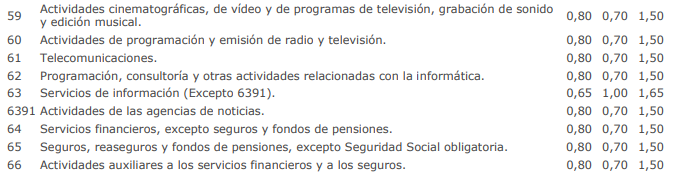
\includegraphics[scale=0.5]{img/AT.png} \\
                \caption{Costes de la empresa - Accidentes de trabajo}
                \label{Costes de la empresa - Accidentes de trabajo}
               \end{minipage}
            \end{figure}
            
            \item\textit {Desempleo:}\\
            Cotización a la seguridad social que paga la empresa por desempleo.\\
            \begin{figure}[h]
              \begin{minipage}{1.3\textwidth}
                \centering
                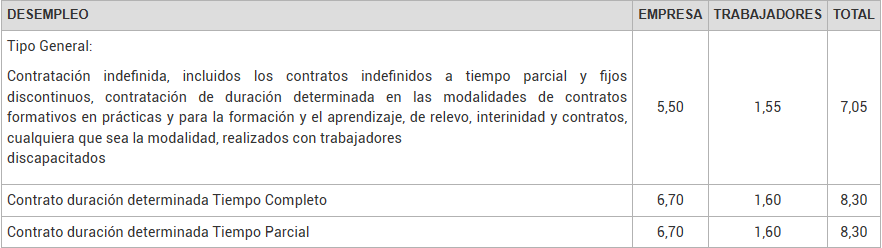
\includegraphics[scale=0.4]{img/Desempleo.png} \\
                \caption{Costes de la empresa - Desempleo}
                \label{Costes de la empresa - Desempleo}
               \end{minipage}
            \end{figure}
            
            \item\textit {Fondo de Garantía Salarial (Fogasa):}\\
            Porcentaje que paga la empresa al Ministerio de Trabajo, Migraciones y Seguridad Social para que, en el caso de declararse la empresa insolvente o en concurso de acreedores, se le paguen a los trabajadores los salarios o indemnizaciones pendientes de abonar.\\
            \begin{figure}[ht]
              \begin{minipage}{1.2\textwidth}
                \centering
                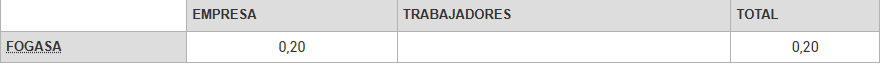
\includegraphics[scale=0.5]{img/Fogasa.png} \\
                \caption{Costes de la empresa - Fogasa}
                \label{Costes de la empresa - Fogasa}
               \end{minipage}
            \end{figure}
            
            \item\textit{} {Formación profesional:}\\
            Cotización que cubre la cuota de necesidades formativas del trabajador.
            \begin{figure}[ht]
              \begin{minipage}{1.2\textwidth}
                \centering
                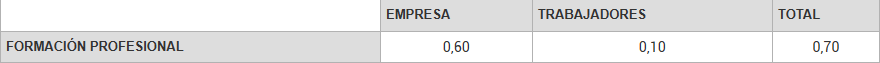
\includegraphics[scale=0.5]{img/FormacionProfesional.png} \\
                \caption{Costes de la empresa - Formación profesional}
                \label{Costes de la empresa - Formación profesional}
               \end{minipage}
            \end{figure}
        \end{enumerate}
    \end{enumerate}
    A continuación, se muestran las tablas de lo que la empresa debería pagar en el caso de contratar al alumno.
     \tablaSmallSinColores{Viabilidad económica - Costes del alumno}{p{5cm} p{4cm} p{4cm}}{Viabilidad económica - Costes del alumno}
        {
          \multicolumn{1}{p{5cm}}{\textbf{Concepto económico}} & \textbf{Coste(€)}\\
         }
         {
        Salario mensual neto & \multicolumn{1}{r}{1950.00€/mes}\\
        Contingencias comunes (23,60\%) & \multicolumn{1}{r}{460.20€/mes}\\
        AT (1,5\%) & \multicolumn{1}{r}{29.25€/mes}\\
        Desempleo (5,50\%)  & \multicolumn{1}{r}{107.25€/mes}\\
        FOGASA (0,20\%) & \multicolumn{1}{r}{3,90€/mes}\\
        Formación profesional (0,60\%) & \multicolumn{1}{r}{11.70€/mes}\\\hline
        \textbf{Salario mensual bruto}  & \multicolumn{1}{r}{2562.10€/mes}\\
        \textbf{Coste 5 meses}  & \multicolumn{1}{r}{12810.5€/5 meses}\\
        }
    No se ha tenido en cuenta la dedicación de los tutores como coste imputable al proyecto puesto que forma parte de las tareas propias de tutorización de la asignatura de proyecto de fin de grado.


    \begin{itemize}
        \item\textit{} {COSTES DE HARDWARE Y SOFTWARE}\\
        Se deben estimar los costes del hardware y software necesario para el desarrollo del proyecto.\\
        Solo deberán tenerse en cuenta en caso de contratación por cuenta ajena, ya que dentro del precio del profesional con cuenta propia vienen incluidos también estos costes.  
        \begin{itemize}
            \item\textit{} {COSTES DE HARDWARE}\\
            Para el desarrollo del TFG se emplea un ordenador portatil ASUS intel CORE i3, un monitor ASUS de 23 pulgadas y como complemento un ratón Logitech.
            Se estima la vida útil de los mismos en 5 años, es decir, cada año se devalúa un 1/5, por lo tanto se calculan las amortizaciones de los meses de uso durante el proyecto (5 meses) de la siguiente manera:


                \tablaSmallSinColores{Costes de hardware y software - Costes de hardware}{p{4cm} p{1cm} p{1cm} p{1cm}}{Costes de hardware y software - Costes de hardware}
                {
                  \multicolumn{1}{p{3cm}}{\textbf{Concepto económico}} &  \multicolumn{1}{p{1cm}}{\textbf{Coste(€)}} & \multicolumn{1}{p{1cm}}\textbf{Amortización(€)} & \multicolumn{1}{p{1cm}}\textbf{Años}\\
                 }
                 {
                Ordenador ASUS & \multicolumn{1}{r}{550}\ & \multicolumn{1}{r}{45,83}\ & \multicolumn{1}{r}{5 años}\\
                Monitor ASUS & \multicolumn{1}{r}{106}\ & \multicolumn{1}{r}{8,83}\ & \multicolumn{1}{r}{5 años}\\
                Ratón LOGITECH & \multicolumn{1}{r}{17,99}\
                 & \multicolumn{1}{r}{1,49}\ & \multicolumn{1}{r}{5 años}\\\hline
                \textbf{Total}  & \multicolumn{1}{r}{673,99} & \multicolumn{1}{r}{56,15} & \multicolumn{1}{r}{5 años}\\
                }

            \item\textit{} {COSTES DE SOFTWARE}\\
            Igualmente, se van a calcular los costes que supone el software que se utiliza para la realización del proyecto, tanto para el despliegue de la aplicación web, como para la base de datos a través de Heroku. También se estimará la vida útil de los mismos en 5 años.

                \tablaSmallSinColores{Trabajador por cuenta ajena - Costes de software}{p{6cm} p{2cm}}{Trabajador por cuenta ajena - Costes de software}
                {
                  \multicolumn{1}{p{6cm}}{\textbf{Concepto económico}} &  \multicolumn{1}{p{2cm}}{\textbf{Coste(€)}} \\
                 }
                 {
                Windows 10 & \multicolumn{1}{r}{1,50}\\
                Heroku app & \multicolumn{1}{r}{7,00}\\
                Heroku PostgreSQL & \multicolumn{1}{r}{9,00}\\\hline
                \textbf{Total}  & \multicolumn{1}{r}{17,50}\\
                }

        \end{itemize}
    \end{itemize}
    \begin{itemize}
    \item\textit{} {COSTES TOTALES}\\
    Se calculan los gastos totales que derivan de la contratación del alumno, la compra de los sistemas hardware y los sistemas software.

    

            \tablaSmallSinColores{Trabajador por cuenta ajena - Costes totales}{p{4cm} p{1cm} p{1cm} p{1cm}}{Trabajador por cuenta ajena - Costes totales}
            {
              \multicolumn{1}{p{3cm}}{\textbf{Concepto económico}} &  \multicolumn{1}{p{1cm}}{\textbf{Coste(€)}} & \multicolumn{1}{p{1cm}}\textbf{Amortización(€)} & \multicolumn{1}{p{1cm}}\textbf{Años}\\
             }
             {
            Coste del alumno & \multicolumn{1}{r}{12810,5}\ & \multicolumn{1}{r}{-}\ & \multicolumn{1}{r}{-}\\
            Coste hardware & \multicolumn{1}{r}{673,99}\ & \multicolumn{1}{r}{87,62}\ & \multicolumn{1}{r}{5 años}\\
            Coste software & \multicolumn{1}{r}{17,50}\
             & \multicolumn{1}{r}{-}\ & \multicolumn{1}{r}{-}\\\hline
            \textbf{Total}  & \multicolumn{1}{r}{13501,99} & \multicolumn{1}{r}{92,04} & \multicolumn{1}{r}{5 años}\\
            }

    \end{itemize}
\end{itemize}


\subsubsection{BENEFICIOS}
La página web se va a distribuir de manera libre y gratuita utilizándose principalmente en la investigación sobre el impacto en Twitter de los Bienes de Interés Cultural del Camino de Santiago Francés en su tramos castellano leonés, por lo que no se generarán beneficios.
La página web tampoco incluye anuncios publicitarios, por lo que tampoco se obtendrán beneficios de los mismos.

\subsection{Viabilidad legal}
Además de estimar los costes que supone la realización del proyecto, se necesitan las licencias del software para cumplir con los requisitos legales.\\
Las herramientas utilizadas en este proyecto pueden verse en la siguiente tabla con sus respectivas versiones y licencias:

\begin{table}[ht!]
    \centering
    \begin{tabular}{c|c|c}
         \hline
         \textbf{Herramientas} & \textbf{Versión} &\textbf{Licencia} \\\hline
         {GitHub} &{3.1.2} &{GNU} \\\hline 
         {Flask} &{2.2.2} &{BSD} \\\hline
         {Leaflet} &{1.8.0} &{BSD 2-Clause Simplified} \\\hline
         {Twitter developer} &{-} &{Licencia de uso } \\\hline
         {Heroku} &{-} &{Licencia de servicio} \\\hline
         {PostgreSQL} &{6.18} &{PostgreSQL License} \\\hline 
         {Bootstrap} &{12.16.1} &{MIT} \\\hline 
         {Plotly} &{5.13.0} &{MIT} \\\hline
         {Pandas} &{1.5.2} &{BSD} \\\hline 
         {Werkzeug} &{9.1.0} &{BSD-3-Clause New} \\\hline
         {Psycopg2} &{2.9.5} &{LGPL} \\\hline 
         {Dotenv} &{0.21.0} &{BSD-2-Clause Simplified} \\\hline 
         {Dateutil} &{2.8.2} &{BSD-3-Clause} \\\hline 
         {Jinja2} &{3.1.2} &{BSD-3-Clause} \\\hline 
         {Sentiment-Analysis-Spanish} &{0.0.25} &{MIT} \\\hline 
         {requests} &{2.28.2} &{Apache 2.0} \\\hline 
    \end{tabular}    \caption{Viabilidad legal - Licencias}
    \label{tab:my_label}
\end{table}

A continuación, se detallan las características de cada una de las licencias nombradas anteriormente y cual es su funcionamiento:\\

\begin{enumerate}
    \item {\textbf{GNU \textit{Git}}\textit{("GNU General Public License")}}\cite{GNU}\\
    Licencia de software libre, la cual permite modificar, utilizar y distribuir código fuente siempre que se incluyan los créditos de autor.
    Además, cualquier cambio o actualización del código fuente debe ser libre y gratuito.
    \item {\textbf{BSD }\textit{("Berkeley Source Distribution")}}\cite{BSD}\\
    Licencia de software libre, la cual permite copiar, modificar y distribuir código fuente siempre que se reserve una copia de la declaración original de derechos de autor.Además, permite el uso del código fuente en software no libre
    \item {\textbf{BSD 2}\textit{("Berkeley Source Distribution 2")}}\cite{BSD2}\\
    Licencia de software libre casi ilimitada, la cual permite copiar, modificar y distribuir código fuente siempre que se incluyan los derechos de autor.
     \item {\textbf{BSD 3 }\textit{("Berkeley Source Distribution 3")}}\cite{BSD3}\\
    Licencia de software libre casi ilimitada, que presenta las restricciones de incluir el texto entero de la licencia y de mencionar los derechos de autor original.
    \item {\textbf{Licencia de uso } \textit{Twitter Developer}}\cite{LicenciaUso}\\
    Licencia que se acepta al comenzar el uso de la API de Twitter, la cual incluye el uso permitido, la responsabilidad legal y la terminación de servicio.
    Además, se deben cumplir las políticas de Twitter, entre ellas las de contenido, privacidad y seguridad.
    \item {\textbf{Licencia de servicio } \textit{Heroku}}\cite{LicenciaServicio}\\
    Licencia que se acepta al comenzar el servicio con Heroku (propiedad de Salesforce), la cual incluye el uso permitido, la responsabilidad legal y la terminación de servicio.
    \item {\textbf{Licencia } \textit{PostgreSQL}}\cite{LicenciaPostgreSQL}\\\
    Licencia similar a MIT o BSD. Se trata de una licencia de código abierto con permisos de uso, modificación, copia y distribución siempre que se incluyan los créditos de autor.
    \item {\textbf{MIT } \textit{("Massachusetts Institute of Technology")}}\cite{MIT}\\
    Se concede el permiso de usar, copiar, modificar, fusionar, publicar, distribuir, sublicenciar y/o vender copias del Software.
    \item {\textbf{LGPL }\textit{("Lesser General Public License")}}\cite{LGPL}\\
    Licencia de software libre que permite la permite copia, distribución o modificación de código fuente; el resto de acciones no estarán cubiertas por esta licencia.
    \item {\textbf{Apache 2.0 }}\cite{Apache}\\
    Licencia de software libre que permite la permite  utilizar, copiar, modificar y distribuir el software, incluyendo una copia de la licencia en la distribución y con la obligación de notificar el uso patentado del software.
\end{enumerate}
La licencia que se ha creido más conveniente para el proyecto ha sido la licencia MIT, ya que es una licencia permisiva que permite a los usuarios realizar diversas acciones incluyendo el uso comercial, la modificación, la distribución y el uso privado, y es compatible con todas las licencias de las herramientas utilizadas en el proyecto.





\apendice{Especificación de Requisitos}

\section{Introducción}

La Especificación de Requisitos Software \textit{(ERS)} es el documento intermediario entre los desarrolladores y los clientes. 
En este se exponen los objetivos respecto al software y los requisitos para conseguir el resultado esperado. \\
En las siguientes secciones se analizarán cada uno de los requisitos necesarios, tanto funcionales como no funcionales, con sus respectivos casos de uso.

\section{Objetivos generales}
Al comienzo del desarrollo del proyecto, se marcaron unos objetivos a cumplir:
\begin{enumerate}
    \item \textbf{Aplicación web:}\\
    Crear una página web funcional que permita realizar el análisis de datos extraídos de Twitter.
    \item \textbf{API de Twitter:}\\
    Conectar con la API de Twitter para la obtención de datos de la red social Twitter.
    \item \textbf{Base de datos:}\\
    Conectarse con una base de datos para almacenar la información extraída de Twitter y más tarde recuperarla para la realización de estadísticas.
    \item \textbf{Patrimonio histórico \textit{BICs}:}\\
    Selección del patrimonio histórico del tramo del camino Francés en Castilla y León de la que se requieren los gráficos estadísticos.
    \item \textbf{Estadísticas temporales:}\\
    Visualizar gráficamente la información almacenada en la base datos.
    \item \textbf{Análisis de sentimientos:}\\
    Calcular un índice de sentimiento (negativo o positivo) de cada tweet. Visualizar los valores medios de sentimiento de los tweets de cada patrimonio.
\end{enumerate}
\section{Catalogo de requisitos}
A continuación se detallarán cada uno de los requisitos, tanto funcionales como no funcionales de la aplicación del proyecto.
\subsection{Requisitos funcionales}
Los requisitos funcionales son cada una de las tareas que satisfacen las necesidades del usuario y que pueden ser detectadas por el mismo. \\
Estas se han desarrollado a lo largo del proyecto hasta cumplir con su funcionalidad.

\begin{itemize}
    \item \textbf{RF1-Visualización de datos estadísticos:} La aplicación debe ser capaz de mostrar los datos estadísticos de los tweets.
    \begin{itemize}
        \item \textbf{RF1.1-Gráfico temporal:} La aplicación debe mostrar un gráfico de los tweets sobre el patrimonio elegido entre un periodo de tiempo.
        \item \textbf{RF1.2-Gráfico porcentual:} La aplicación debe ser capaz de mostrar un gráfico circular del porcentaje de tweets sobre el patrimonio elegido respecto al resto de patrimonios.
        \item \textbf{RF1.3-Gráfico de datos públicos:} La aplicación debe ser capaz de mostrar un gráfico de barras comparando los parámetros públicos de los tweets del BIC elegido entre un periodo de tiempo.
        \item \textbf{RF1.4-Selección de fechas:} El usuario debe poder seleccionar las fechas entre las que requiere las estadísticas patrimoniales.
        \item \textbf{RF1.5-Análisis de sentimientos:} La aplicación debe ser capaz de mostrar gráficamente los valores medios de sentimiento de los tweets de cada patrimonio.
        \item \textbf{RF1.6-Gráfico de estadísticas generales:} La aplicación debe ser capaz de mostrar gráficamente el total de los tweets de todos los BICs.
    \end{itemize}
    \item \textbf{RF2-Mapa de patrimonios:} La aplicación deberá mostrar en un mapa cada uno de los BICs en su localización real.
    \begin{itemize}
        \item \textbf{RF2.1-Mostrar nombre de patrimonio:} El usuario debe poder ver el nombre del BIC al que se refiere cada una de las localizaciones.
        \item \textbf{RF2.2-Selección de BIC:} El usuario debe poder seleccionar un bien de interés cultural en el mapa y realizar estadísticas.
    \end{itemize}
    \item \textbf{RF3-Barra navegadora:} La aplicación debe tener una barra navegadora para redireccionarse a otras páginas de la aplicación.
    \begin{itemize}
        \item \textbf{RF3.1-Inicio:} La barra navegadora debe contener un botón que redireccione a la página de inicio.
        \item \textbf{RF3.2-Administrador:} La barra de navegación debe tener un desplegable con las opciones que, siendo administrador, se pueden realizar.
        \begin{itemize}
            \item \textbf{RF3.2.1-Iniciar sesión:} La aplicación debe ser capaz, a través del botón de la barra navegadora, de redireccionar a la página de \textit{'Iniciar sesión'}.
            \item \textbf{RF3.2.2-Cerrar sesión:} La aplicación debe ser capaz, a través del botón de la barra navegadora, de redireccionar a la página de \text{'Cerrar sesión'}.
            \item \textbf{RF3.2.3-Opciones del Administrador:} La aplicación debe ser capaz, a través del botón de la barra navegadora, de redireccionar a la página de opciones del Administrador.
        \item \textbf{RF3.3-Estadísticas generales:} La barra navegadora debe contener un botón que redireccione a la página de estadísticas generales.
            
        \end{itemize}
    \end{itemize}
    \item \textbf{RF4-Iniciar sesión:} La aplicación debe ser capaz de comprobar si las credenciales de rol administrador son correctas.
    \item \textbf{RF5-Opciones de rol Administrador:} Si las credenciales de
administrador son correctas, la aplicación debe proporcionar las posibles acciones que puede realizar.
    \begin{itemize}
        \item \textbf{RF5.1-Crear base de datos:} El rol administrador debe poder crear una base de datos de acuerdo a unos parámetros prestablecidos.
        \begin{itemize}
            \item \textbf{RF5.1.1-Fecha de inicio:} El administrador debe poder elegir la fecha desde la que quiere que se obtengan los datos de Twitter.
            \item \textbf{RF5.1.2-Número de peticiones:} El administrador debe poder elegir el máximo número de peticiones a realizar durante el periodo de tiempo permitido por la API.
            \item \textbf{RF5.1.3-Tiempo de espera:} El administrador debe poder elegir cuánto tiempo desea que espere la aplicación una vez realizadas el número de peticiones elegidas anteriormente para realizar el siguiente grupo de peticiones.
            \item \textbf{RF5.1.4-Tiempo de duración de cada petición:} El administrador debe poder elegir cuál va a ser la duración de cada petición.
        \end{itemize}
        \item \textbf{RF5.2-Actualizar base de datos:} El administrador debe poder actualizar la base de datos desde la última fecha de la que se recopiló información hasta la fecha actual.
        \begin{itemize}
            \item \textbf{RF5.2.1-Número de peticiones:} El administrador debe poder elegir el máximo número de peticiones a realizar durante el periodo de tiempo permitido por la API.
            \item \textbf{RF5.2.2-Tiempo de espera:} El administrador debe poder elegir cuánto tiempo desea que espere la aplicación una vez realizadas el número de peticiones elegidas anteriormente para realizar el siguiente grupo de peticiones.
            \item \textbf{RF5.2.3-Tiempo de duración de cada petición:} El administrador debe poder elegir cuál va a ser la duración de cada petición.
        \end{itemize}
        \item \textbf{RF5.3-Cerrar sesión:} El administrador debe poder salir de la sesión actual.
    \end{itemize}
\end{itemize}
\subsection{Requisitos no funcionales}
Los requisitos no funcionales son aquellos que se le solicitan al sistema y en los que no influyen las necesidades del usuario \\
\begin{itemize}
    \item \textbf{RNF1-Escalabilidad:} La aplicación debe ser fácilmente ampliable de cara a añadir nuevas funcionalidades o desarrollos.
    \item \textbf{RNF2-Mantenibilidad:} La aplicación debe permitir actualizaciones y poder mantener las funcionalidades ya desarrolladas.
    \item \textbf{RNF3-Seguridad:} La aplicación no debe permitir la modificación de funcionalidades a usuarios no autorizados.
    \item \textbf{RNF4-Portabilidad:} La aplicación debe poder ejecutarse en distintas plataformas sin necesidad de aplicar cambios.
    \item \textbf{RNF5-Compliance:} La aplicación debe adaptarse a las leyes establecidas como, por ejemplo, la protección de datos.
\end{itemize}
\section{Especificación de requisitos}
Se van a analizar las especificaciones de requisitos a través del análisis de los actores por diagramas de uso con sus respectivas tablas.
\subsection{Diagrama de caso de uso}
Se muestra a través de un diagrama de caso de uso los actores y los requisitos accesibles de cada rol.

\begin{landscape}
    \begin{figure}[h!]
        \centering
        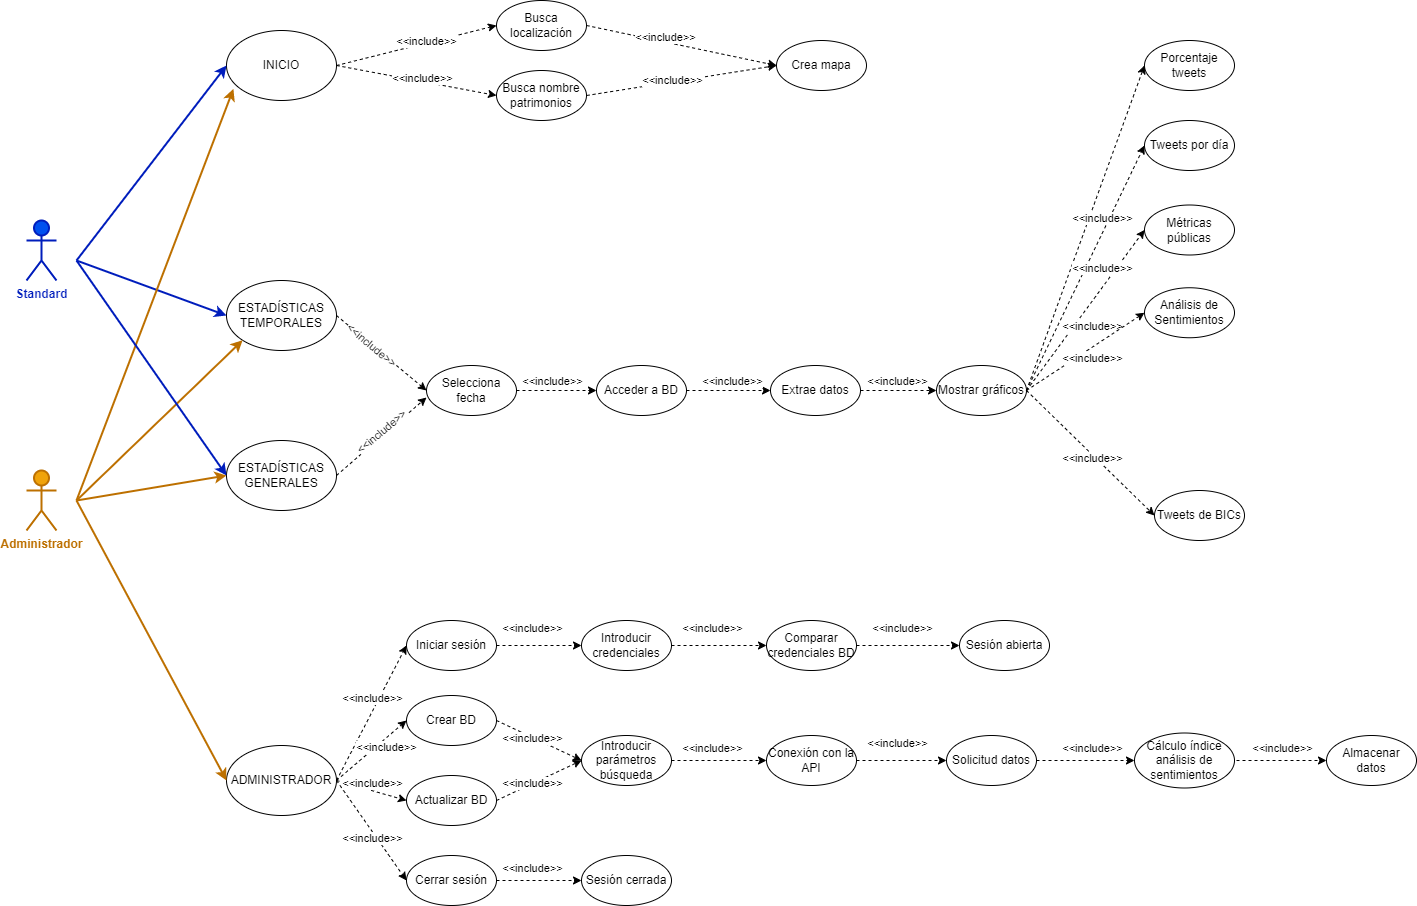
\includegraphics[scale=0.4]{img/casosDeUso.png} \\
        \caption{Especificación de requisitos - Diagrama de caso de uso}
        \label{Especificación de requisitos - Diagrama de caso de uso}
    \end{figure}
\end{landscape}


\subsection{Tablas de caso de uso}
Se muestra a través de tablas, la información de cada requisito del diagrama con sus respectivos parámetros.
% Caso de Uso 1 -> INICIO.
\begin{table}[h!]
	\centering
	\begin{tabularx}{\linewidth}{ p{0.21\columnwidth} p{0.71\columnwidth} }
		\toprule
		\textbf{CU-1}    & \textbf{Inicio}\\
		\toprule
		\textbf{Versión}              & 1.0    \\
		\textbf{Autor}                & Usuario y administrador \\
		\textbf{Requisitos asociados} & RF2, RF3, RF3.1 \\
		\textbf{Descripción}          & Página principal de la aplicación. \\
		\textbf{Precondición}         & Se debe abrir la aplicación en un navegador web. \\
		\textbf{Acciones}             &
		\begin{enumerate}
			\def\labelenumi{\arabic{enumi}.}
			\tightlist
			\item Entrar en el navegador.
			\item Escribir la dirección web.
                \item Si se encuentra en otra página de la aplicación, pulsar en la barra navegadora el boton\textit{'Inicio'}.
		\end{enumerate}\\
		\textbf{Postcondición}        &  -\\
		\textbf{Excepciones}          &  -\\
		\textbf{Importancia}          & Alta \\
		\bottomrule
	\end{tabularx}
	\caption{CU-1 Inicio}
\end{table}
% Caso de Uso 1.1 -> BUSCA LOCALIZACIÓN.
\begin{table}[h!]
	\centering
	\begin{tabularx}{\linewidth}{ p{0.21\columnwidth} p{0.71\columnwidth} }
		\toprule
		\textbf{CU-1.1}    & \textbf{Busca localización}\\
		\toprule
		\textbf{Versión}              & 1.0    \\
		\textbf{Autor}                & Usuario y administrador \\
		\textbf{Requisitos asociados} & RF2, RF3, RF3.1 \\
		\textbf{Descripción}          & Busqueda de localización \\
		\textbf{Precondición}         & Estar en el \textit{'Inicio'}. \\
		\textbf{Acciones}             &
		\begin{enumerate}
			\def\labelenumi{\arabic{enumi}.}
			\tightlist
                \item El programa busca en el csv \textit{inventario\_01} la localización de cada patrimonio.
		\end{enumerate}\\
		\textbf{Postcondición}        &  -\\
		\textbf{Excepciones}          &  -\\
		\textbf{Importancia}          & Baja \\
		\bottomrule
	\end{tabularx}
	\caption{CU-1.1 Busca localización}
\end{table}
% Caso de Uso 1.2 -> BUSCA NOMBRES PATRIMONIOS.
\begin{table}[h!]
	\centering
	\begin{tabularx}{\linewidth}{ p{0.21\columnwidth} p{0.71\columnwidth} }
		\toprule
		\textbf{CU-1.2}    & \textbf{Busca nombre patrimonios}\\
		\toprule
		\textbf{Versión}              & 1.0    \\
		\textbf{Autor}                & Usuario y administrador \\
		\textbf{Requisitos asociados} & RF2, RF3, RF3.1 \\
		\textbf{Descripción}          & Busqueda de nombres de patrimonios \\
		\textbf{Precondición}         & Estar en el \textit{'Inicio'}. \\
		\textbf{Acciones}             &
		\begin{enumerate}
			\def\labelenumi{\arabic{enumi}.}
			\tightlist
                \item El programa busca en el csv \textit{inventario\_01} los nombres de cada patrimonio.
		\end{enumerate}\\
		\textbf{Postcondición}        &  -\\
		\textbf{Excepciones}          &  -\\
		\textbf{Importancia}          & Baja \\
		\bottomrule
	\end{tabularx}
	\caption{CU-1.2 Busca nombre patrimonios}
\end{table}
% Caso de Uso 1.2.1 -> CREAR MAPA.
\begin{table}[h!]
	\centering
	\begin{tabularx}{\linewidth}{ p{0.21\columnwidth} p{0.71\columnwidth} }
		\toprule
		\textbf{CU-1.2.1}    & \textbf{Crear mapa}\\
		\toprule
		\textbf{Versión}              & 1.0    \\
		\textbf{Autor}                & Usuario y administrador \\
		\textbf{Requisitos asociados} & RF2, RF2.1, RF3, RF3.1 \\
		\textbf{Descripción}          & Mapa dinámico con los patrimonios históricos geolocalizados. \\
		\textbf{Precondición}         & Entrar en la página inicio. \\
		\textbf{Acciones}             &
		\begin{enumerate}
			\def\labelenumi{\arabic{enumi}.}
			\tightlist
			\item Entrar en la página \textit{'Inicio'}
			\item Mover con el ratón el mapa
		\end{enumerate}\\
		\textbf{Postcondición}        &  -\\
		\textbf{Excepciones}          &  -\\
		\textbf{Importancia}          & Media \\
		\bottomrule
	\end{tabularx}
	\caption{CU-1.1 Visualización de mapa.}
\end{table}
% Caso de Uso 1.2 -> ELECCION DE PATRIMONIO HISTÓRICO.
\begin{table}[h!]
	\centering
	\begin{tabularx}{\linewidth}{ p{0.21\columnwidth} p{0.71\columnwidth} }
		\toprule
		\textbf{CU-1.2}    & \textbf{Elección de patrimonio histórico}\\
		\toprule
		\textbf{Versión}              & 1.0    \\
		\textbf{Autor}                & Usuario y administrador \\
		\textbf{Requisitos asociados} & RF2, RF2.1, RF2.2 RF3, RF3.1\\
		\textbf{Descripción}          & Elección del patrimonio histórico sobre el mapa. \\
		\textbf{Precondición}         & Entrar en la página inicio. \\
		\textbf{Acciones}             &
		\begin{enumerate}
			\def\labelenumi{\arabic{enumi}.}
			\tightlist
			\item Entrar La página \textit{'Inicio'}
			\item Buscar con el rotón, en el mapa, el patrimonio deseado.
            \item Hacer click sobre él
		\end{enumerate}\\
		\textbf{Postcondición}        &  Hacer click sobre el \textit{'pop up'}\\
		\textbf{Excepciones}          &  Solo se ubican los BICs del Camino de Santiago en la etapa de Castilla y León.\\
		\textbf{Importancia}          & Media \\
		\bottomrule
	\end{tabularx}
	\caption{CU-1.2 Elección de patrimonio histórico.}
\end{table}

% Caso de Uso 2 -> ESTADÍSTICAS TEMPORALES.
\begin{table}[h!]
	\centering
	\begin{tabularx}{\linewidth}{ p{0.21\columnwidth} p{0.71\columnwidth} }
		\toprule
		\textbf{CU-2}    & \textbf{Estadísticas temporales}\\
		\toprule
		\textbf{Versión}              & 1.0    \\
		\textbf{Autor}                & Usuario y administrador \\
		\textbf{Requisitos asociados} & RF1, RF2, RF2.1, RF2.2, RF3, RF3.1\\
		\textbf{Descripción}          & Ventana de la aplicación que contiene todos los gráficos estadísticos sobre el BIC elegido anteriormente, pudiendo cambiar de periodo temporal.  \\
        \textbf{Precondición}         & 
        \begin{enumerate}
			\def\labelenumi{\arabic{enumi}.}
			\tightlist
			\item Entrar en la página \textit{'Inicio'}
			\item Buscar con el ratón, en el mapa, el BIC deseado.
            \item Hacer click sobre él
            \item Hacer click sobre el link incluido en el \textit{pop up'} 
            
		\end{enumerate}\\
		
		\textbf{Acciones}             &
		\begin{enumerate}
			\def\labelenumi{\arabic{enumi}.}
			\tightlist
			\item Visualizar las gráficas.
                \item Selección de fecha.
            
            \item Si se quiere regresar a la página de \textit{'Inicio'}, pulsar sobre el botón de \textit{'Volver'}

		\end{enumerate}\\
		\textbf{Postcondición}        &  Dar al botón \textit{'Volver'}\\
		\textbf{Excepciones}  &
            \begin{enumerate}
                \item La fecha de inicio debe ser anterior a la final.
                \item La base de datos no puede estar vacía.
            \end{enumerate}  \\
            
		\textbf{Importancia}          & Alta \\
		\bottomrule
	\end{tabularx}
	\caption{CU-2 Estadísticas temporales}
\end{table}
% Caso de Uso 3 -> ESTADÍSTICAS GENERALES.
\begin{table}[h!]
	\centering
	\begin{tabularx}{\linewidth}{ p{0.21\columnwidth} p{0.71\columnwidth} }
		\toprule
		\textbf{CU-3}    & \textbf{Estadísticas generales}\\
		\toprule
		\textbf{Versión}              & 1.0    \\
		\textbf{Autor}                & Usuario y administrador \\
		\textbf{Requisitos asociados} & RF1, RF1.6, RF2, RF2.1, RF2.2, RF3, RF3.1, RF3.3\\
		\textbf{Descripción}          & Ventana de la aplicación que contiene el gráfico estadístico comparando todos los BICs, pudiendo cambiar de periodo temporal.  \\
        \textbf{Precondición}         & 
        \begin{enumerate}
			\def\labelenumi{\arabic{enumi}.}
			\tightlist
			\item Entrar en la página \textit{'Inicio'}
			\item En la barra navegadora pulsar sobre \textit{'Estadísticas generales'}.
            
		\end{enumerate}\\
		
		\textbf{Acciones}             &
		\begin{enumerate}
			\def\labelenumi{\arabic{enumi}.}
			\tightlist
			\item Visualizar la gráfica.
                \item Selección de fecha.
            
            \item Si se quiere regresar a la página de \textit{'Inicio'}, pulsar sobre el botón de \textit{'Volver'}

		\end{enumerate}\\
		\textbf{Postcondición}        &  Dar al botón \textit{'Volver'}\\
		\textbf{Excepciones}  &
            \begin{enumerate}
                \item La fecha de inicio debe ser anterior a la final.
                \item La base de datos no puede estar vacía.
            \end{enumerate}  \\
            
		\textbf{Importancia}          & Alta \\
		\bottomrule
	\end{tabularx}
	\caption{CU-3 Estadísticas generales}
\end{table}
% Caso de Uso 2.1 -> SELECCIONA FECHA.
\begin{table}[h!]
	\centering
	\begin{tabularx}{\linewidth}{ p{0.21\columnwidth} p{0.71\columnwidth} }
		\toprule
		\textbf{CU-2.1/3.1}    & \textbf{Selecciona fecha}\\
		\toprule
		\textbf{Versión}              & 1.0    \\
		\textbf{Autor}                & Usuario y administrador \\
		\textbf{Requisitos asociados} & RF1, RF1.4, RF2, RF2.1, RF2.2, RF3, RF3.1\\
		\textbf{Descripción}          & Cambio de fechas para realizar los gráficos temporales.  \\
        \textbf{Precondición}         & 
        \begin{enumerate}
			\def\labelenumi{\arabic{enumi}.}
			\tightlist
			\item Entrar en la página \textit{'Inicio'}
			\item Buscar con el ratón, en el mapa, el BIC deseado.
            \item Hacer click sobre él
            \item Hacer click sobre el link incluido en el \textit{'pop up'} 
            
		\end{enumerate}\\
		
		\textbf{Acciones}             &
		\begin{enumerate}
			\def\labelenumi{\arabic{enumi}.}
			\tightlist
			\item Seleccionar la fecha de inicio en el primer \textit{'input'} que aparece en la parte superior.
                \item Seleccionar la fecha de inicio en el primer \textit{'input'} que aparece en la parte superior.

		\end{enumerate}\\
		\textbf{Postcondición}        &  Dar al botón \textit{'Buscar'} \\
		\textbf{Excepciones}          &  La fecha de inicio debe ser anterior a la final.\\
		\textbf{Importancia}          & Media \\
		\bottomrule
	\end{tabularx}
	\caption{CU-2.1/3.1 Selecciona fecha}
\end{table}
% Caso de Uso 2.1.1 -> ACCEDER A BASE DE DATOS.
\begin{table}[h!]
	\centering
	\begin{tabularx}{\linewidth}{ p{0.21\columnwidth} p{0.71\columnwidth} }
		\toprule
		\textbf{CU-2.1.1/3.1.1}    & \textbf{Acceder a base de datos}\\
		\toprule
		\textbf{Versión}              & 1.0    \\
		\textbf{Autor}                & Usuario y administrador \\
		\textbf{Requisitos asociados} & RF1, RF1.4, RF2, RF2.1, RF2.2, RF3, RF3.1\\
		\textbf{Descripción}          & Se realiza la conexión con la base de datos para realizar operaciones  \\
        \textbf{Precondición}         & 
        \begin{enumerate}
			\def\labelenumi{\arabic{enumi}.}
			\tightlist
			\item Entrar en la página \textit{'Inicio'}
			\item Buscar con el ratón, en el mapa, el BIC deseado.
            \item Hacer click sobre él
            \item Hacer click sobre el link incluido en el \textit{'pop up'} 
            \item Si el usuario ya se encuentra en la página de estadísticas, para realizar la conexión con la base de datos antes se debe pulsar al botón \textit{'buscar'}.
            
		\end{enumerate}\\
		
		\textbf{Acciones}             &
		\begin{enumerate}
			\def\labelenumi{\arabic{enumi}.}
			\tightlist
			\item De manera interna se realiza la conexión con la base de datos mediante psycopg2
            
		\end{enumerate}\\
		\textbf{Postcondición}        &  - \\
		\textbf{Excepciones}          &  La fecha de inicio debe ser anterior a la final.\\
		\textbf{Importancia}          & Alta \\
		\bottomrule
	\end{tabularx}
	\caption{CU-2.1.1/3.1.1 Acceder a base de datos}
\end{table}

% Caso de Uso 2.1.1.1 -> EXTRAE DATOS.
\begin{table}[h!]
	\centering
	\begin{tabularx}{\linewidth}{ p{0.21\columnwidth} p{0.71\columnwidth} }
		\toprule
		\textbf{CU-2.1.1.1/3.1.1.1}    & \textbf{Extrae datos}\\
		\toprule
		\textbf{Versión}              & 1.0    \\
		\textbf{Autor}                & Usuario y administrador \\
		\textbf{Requisitos asociados} & RF1, RF1.4, RF2, RF2.1, RF2.2, RF3, RF3.1\\
		\textbf{Descripción}          & Se realiza la búsqueda de la información requerida del BIC.  \\
        \textbf{Precondición}         & 
        \begin{enumerate}
			\def\labelenumi{\arabic{enumi}.}
			\tightlist
                \item Seleccionar un BIC.
                \item Seleccionar fechas. 
			\item Tener una conexión con la base de datos.
            
		\end{enumerate}\\
		
		\textbf{Acciones}             &
		\begin{enumerate}
			\def\labelenumi{\arabic{enumi}.}
			\tightlist
			\item Se realizan las búsquedas en la base de datos filtrando por el nombre del BIC y las fechas.
            
		\end{enumerate}\\
		\textbf{Postcondición}        &  - \\
		\textbf{Excepciones}          &  La fecha de inicio debe ser anterior a la final.\\
		\textbf{Importancia}          & Alta \\
		\bottomrule
	\end{tabularx}
	\caption{CU-2.1.1.1/3.1.1.1 Extrae datos}
\end{table}

% Caso de Uso 2.1.1.1.1 -> MOSTRAR GRÁFICOS.
\begin{table}[h!]
	\centering
	\begin{tabularx}{\linewidth}{ p{0.21\columnwidth} p{0.71\columnwidth} }
		\toprule
		\textbf{CU-2.1.1.1.1/3.1.1.1.1}    & \textbf{Mostrar gráficos}\\
		\toprule
		\textbf{Versión}              & 1.0    \\
		\textbf{Autor}                & Usuario y administrador \\
		\textbf{Requisitos asociados} & RF1, RF1.1, RF1.2, RF1.3, RF1.4, RF2, RF2.1, RF2.2, RF3, RF3.1\\
		\textbf{Descripción}          & Se realizan los gráficos con la información obtenida de la base de datos.  \\
        \textbf{Precondición}         & 
        \begin{enumerate}
			\def\labelenumi{\arabic{enumi}.}
			\tightlist
                \item Seleccionar un BIC.
                \item Seleccionar fechas. 
			\item Tener una conexión con la base de datos.
                \item Haber obtenido la información que se ha solicitado.
            
		\end{enumerate}\\
		
		\textbf{Acciones}             &
		\begin{enumerate}
			\def\labelenumi{\arabic{enumi}.}
			\tightlist
			\item Realizar los gráficos según los parámetros establecidos.
            
		\end{enumerate}\\
		\textbf{Postcondición}        &  - \\
		\textbf{Excepciones}          &  La fecha de inicio debe ser anterior a la final.\\
		\textbf{Importancia}          & Alta \\
		\bottomrule
	\end{tabularx}
	\caption{CU-2.1.1.1.1/3.1.1.1.1 Mostrar gráficos}
\end{table}

% Caso de Uso 2.1.1.1.1.1 -> PORCENTAJE DE TWEETS.
\begin{table}[h!]
	\centering
	\begin{tabularx}{\linewidth}{ p{0.21\columnwidth} p{0.71\columnwidth} }
		\toprule
		\textbf{CU-2.1.1.1.1.1}    & \textbf{Porcentaje de tweets}\\
		\toprule
		\textbf{Versión}              & 1.0    \\
		\textbf{Autor}                & Usuario y administrador \\
		\textbf{Requisitos asociados} & RF1, RF1.2, RF1.4, RF2, RF2.1, RF2.2, RF3, RF3.1\\
		\textbf{Descripción}          & Se realiza el gráfico de porcentaje de tweets.  \\
        \textbf{Precondición}         & 
        \begin{enumerate}
			\def\labelenumi{\arabic{enumi}.}
			\tightlist
                \item Seleccionar un BIC.
                \item Seleccionar fechas. 
			\item Tener una conexión con la base de datos.
                \item Haber obtenido la información que se ha solicitado.
            
		\end{enumerate}\\
		
		\textbf{Acciones}             &
		\begin{enumerate}
			\def\labelenumi{\arabic{enumi}.}
			\tightlist
			\item Mostrar el gráfico circular con el porcentaje de tweets del BIC en las fechas seleccionadas respecto al total de datos almacenados en la base de datos de todos los patrimonios.
            
		\end{enumerate}\\
		\textbf{Postcondición}        &  - \\
		\textbf{Excepciones}          &  La fecha de inicio debe ser anterior a la final.\\
		\textbf{Importancia}          & Alta \\
		\bottomrule
	\end{tabularx}
	\caption{CU-2.1.1.1.1.1 Porcentaje de tweets}
\end{table}

% Caso de Uso 2.1.1.1.1.2 -> TWEETS POR DIA.
\begin{table}[h!]
	\centering
	\begin{tabularx}{\linewidth}{ p{0.21\columnwidth} p{0.71\columnwidth} }
		\toprule
		\textbf{CU-2.1.1.1.1.2}    & \textbf{Tweets por día}\\
		\toprule
		\textbf{Versión}              & 1.0    \\
		\textbf{Autor}                & Usuario y administrador \\
		\textbf{Requisitos asociados} & RF1, RF1.1, RF1.4, RF2, RF2.1, RF2.2, RF3, RF3.1\\
		\textbf{Descripción}          & Se realiza el gráfico mostrando los tweets generados por día entre las fechas seleccionadas.  \\
        \textbf{Precondición}         & 
        \begin{enumerate}
			\def\labelenumi{\arabic{enumi}.}
			\tightlist
                \item Seleccionar un BIC.
                \item Seleccionar fechas. 
			\item Tener una conexión con la base de datos.
                \item Haber obtenido la información que se ha solicitado.
            
		\end{enumerate}\\
		
		\textbf{Acciones}             &
		\begin{enumerate}
			\def\labelenumi{\arabic{enumi}.}
			\tightlist
			\item Mostrar el gráfico temporal con el número de tweets del BIC en las fechas seleccionadas almacenado en la base de datos.
            
		\end{enumerate}\\
		\textbf{Postcondición}        &  - \\
		\textbf{Excepciones}          &  La fecha de inicio debe ser anterior a la final.\\
		\textbf{Importancia}          & Alta \\
		\bottomrule
	\end{tabularx}
	\caption{CU-2.1.1.1.1.2 Tweets por día}
\end{table}

% Caso de Uso 2.1.1.1.1.3 -> METRICAS PÚBLICAS
\begin{table}[h!]
	\centering
	\begin{tabularx}{\linewidth}{ p{0.21\columnwidth} p{0.71\columnwidth} }
		\toprule
		\textbf{CU-2.1.1.1.1.3}    & \textbf{Métricas públicas}\\
		\toprule
		\textbf{Versión}              & 1.0    \\
		\textbf{Autor}                & Usuario y administrador \\
		\textbf{Requisitos asociados} & RF1, RF1.3, RF1.4, RF2, RF2.1, RF2.2, RF3, RF3.1\\
		\textbf{Descripción}          & Se realiza el gráfico de barras mostrando las métricas públicas del total de tweets al día entre el periodo de tiempo seleccionado.  \\
        \textbf{Precondición}         & 
        \begin{enumerate}
			\def\labelenumi{\arabic{enumi}.}
			\tightlist
                \item Seleccionar un BIC.
                \item Seleccionar fechas. 
			\item Tener una conexión con la base de datos.
                \item Haber obtenido la información que se ha solicitado.
            
		\end{enumerate}\\
		
		\textbf{Acciones}             &
		\begin{enumerate}
			\def\labelenumi{\arabic{enumi}.}
			\tightlist
			\item Mostrar el gráfico temporal apilado con el número de retweets, replies y likes de los tweets de cada uno de los días en el periodo de tiempo seleccionado.
            
		\end{enumerate}\\
		\textbf{Postcondición}        &  - \\
		\textbf{Excepciones}          &  La fecha de inicio debe ser anterior a la final.\\
		\textbf{Importancia}          & Alta \\
		\bottomrule
	\end{tabularx}
	\caption{CU-2.1.1.1.1.3 Métricas públicas}
\end{table}
% Caso de Uso 2.1.1.1.1.4 -> ANÁLISIS DE SENTIMIENTOS
\begin{table}[h!]
	\centering
	\begin{tabularx}{\linewidth}{ p{0.21\columnwidth} p{0.71\columnwidth} }
		\toprule
		\textbf{CU-2.1.1.1.1.4}    & \textbf{Análisis de sentimientos}\\
		\toprule
		\textbf{Versión}              & 1.0    \\
		\textbf{Autor}                & Usuario y administrador \\
		\textbf{Requisitos asociados} & RF1, RF1.3, RF1.4, RF1.5, RF2, RF2.1, RF2.2, RF3, RF3.1\\
		\textbf{Descripción}          & Se realiza el gráfico semicircular mostrando el valor del análisis de sentimientos de los tweets del BIC seleccionado entre las fechas elegidas.  \\
        \textbf{Precondición}         & 
        \begin{enumerate}
			\def\labelenumi{\arabic{enumi}.}
			\tightlist
                \item Seleccionar un BIC.
                \item Seleccionar fechas. 
			\item Tener una conexión con la base de datos.
                \item Haber obtenido la información que se ha solicitado.
            
		\end{enumerate}\\
		
		\textbf{Acciones}             &
		\begin{enumerate}
			\def\labelenumi{\arabic{enumi}.}
			\tightlist
			\item Realizar la media de los valores del análisis de sentimientos de todos los tweets del BIc entre las fechas seleccionadas.
                \item Mostrar con un gráfico semicircular el valor numérico del análisis de sentimientos.
            
		\end{enumerate}\\
		\textbf{Postcondición}        &  - \\
		\textbf{Excepciones}          &  La fecha de inicio debe ser anterior a la final.\\
		\textbf{Importancia}          & Alta \\
		\bottomrule
	\end{tabularx}
	\caption{CU-2.1.1.1.1.4 Análisis de sentimientos}
\end{table}

% Caso de Uso 3.1.1.1.1.1 -> TWEETS de BICs
\begin{table}[h!]
	\centering
	\begin{tabularx}{\linewidth}{ p{0.21\columnwidth} p{0.71\columnwidth} }
		\toprule
		\textbf{CU-3.1.1.1.1.1}    & \textbf{Tweets de BICs}\\
		\toprule
		\textbf{Versión}              & 1.0    \\
		\textbf{Autor}                & Usuario y administrador \\
		\textbf{Requisitos asociados} & RF1, RF1.2, RF1.4, RF1.6 RF2, RF2.1, RF2.2, RF3, RF3.1, RF3.3\\
		\textbf{Descripción}          & Se realiza el gráfico de total de tweets de los BICs.  \\
        \textbf{Precondición}         & 
        \begin{enumerate}
			\def\labelenumi{\arabic{enumi}.}
			\tightlist
                \item Pulsar en la barra navegadora el botón 'Estadístias generales'.
                \item Seleccionar fechas. 
			\item Tener una conexión con la base de datos.
            
		\end{enumerate}\\
		
		\textbf{Acciones}             &
		\begin{enumerate}
			\def\labelenumi{\arabic{enumi}.}
			\tightlist
			\item Mostrar el gráfico con la comparación de los tweets publicados de todos los BICs entre las fechas seleccionadas.
            
		\end{enumerate}\\
		\textbf{Postcondición}        &  - \\
		\textbf{Excepciones}          &  La fecha de inicio debe ser anterior a la final.\\
		\textbf{Importancia}          & Alta \\
		\bottomrule
	\end{tabularx}
	\caption{CU-3.1.1.1.1.1 Tweets de BICs}
\end{table}
% Caso de Uso 4 -> ADMINISTRADOR.
\begin{table}[h!]
	\centering
	\begin{tabularx}{\linewidth}{ p{0.21\columnwidth} p{0.71\columnwidth} }
		\toprule
		\textbf{CU-4}    & \textbf{Administrador}\\
		\toprule
		\textbf{Versión}              & 1.0    \\
		\textbf{Autor}                & Administrador \\
		\textbf{Requisitos asociados} & RF3.2, RF3.2.1, RF3.2.2, RF3.2.3, RF4.2.4, RF4, RF5, RF5.1, RF5.1.1, RF5.1.2, RF5.1.3, RF5.1.4, RF5.2, RF5.2.1, RF5.2.2, RF5.2.3, RF5.3\\
		\textbf{Descripción}          & Ventana de la aplicación que contiene la acción \textit{'Iniciar sesión'} desde la que se podrán realizar las acciones del rol administrador  \\
        \textbf{Precondición}         & Abrir la aplicación \\
		\textbf{Acciones}             &
		\begin{enumerate}
			\def\labelenumi{\arabic{enumi}.}
			\tightlist
			\item Entrar en la página \textit{'Inicio'}
			\item En la barra navegadora hacer click sobre \textit{'Administrador'} para ver las opciones que se sugieren
		\end{enumerate}\\
		\textbf{Postcondición}     &   
        \begin{enumerate}
			\def\labelenumi{\arabic{enumi}.}
			\tightlist
			\item Hacer \textit{'Iniciar sesión'}
			\item Pulsar una de las opciones del desplegable. 
		\end{enumerate}\\
		\textbf{Excepciones}          & -\\
		\textbf{Importancia}          & Media \\
		\bottomrule
	\end{tabularx}
	\caption{CU-4 Administrador.}
\end{table}




% Caso de Uso 4.1 -> INICIAR SESIÓN
\begin{table}[h!]
	\centering
	\begin{tabularx}{\linewidth}{ p{0.21\columnwidth} p{0.71\columnwidth} }
		\toprule
		\textbf{CU-4.1}    & \textbf{Iniciar sesión}\\
		\toprule
		\textbf{Versión}              & 1.0    \\
		\textbf{Autor}                & Administrador \\
		\textbf{Requisitos asociados} & RF3.2, RF3.2.1, RF4, RF5, RF5.1, RF5.1.1, RF5.1.2, RF5.1.3, RF5.1.4, RF5.2, RF5.2.1, RF5.2.2, RF5.2.3, RF5.3\\
		\textbf{Descripción}          & Permite ver la ventana que posibilita al usuario ingresar con unas credenciales para acceder indentificándose como administrador\\
        \textbf{Precondición}         &  
  		\begin{enumerate}
			\def\labelenumi{\arabic{enumi}.}
			\tightlist
			\item Entrar en la página \textit{'Inicio'}
			\item En la barra navegadora hacer click sobre \textit{'Iniciar sesión'}
		\end{enumerate}\\
		\textbf{Acciones}             &
		\begin{enumerate}
			\def\labelenumi{\arabic{enumi}.}
			\tightlist
			\item Ver pestaña de \textit{'Inicio de sesión'}.
		\end{enumerate}\\
		\textbf{Postcondición}     &   Insertar credenciales \\
		\textbf{Excepciones}          & - \\
		\textbf{Importancia}          & Alta \\
		\bottomrule
	\end{tabularx}
	\caption{CU-4.1 Iniciar sesión}
\end{table}

% Caso de Uso 4.1.1 -> INTRODUCIR CREDENCIALES
\begin{table}[h!]
	\centering
	\begin{tabularx}{\linewidth}{ p{0.21\columnwidth} p{0.71\columnwidth} }
		\toprule
		\textbf{CU-4.1.1}    & \textbf{Introducir credenciales}\\
		\toprule
		\textbf{Versión}              & 1.0    \\
		\textbf{Autor}                & Administrador \\
		\textbf{Requisitos asociados} & RF5, RF5.1, RF5.1.1, RF5.1.2, RF5.1.3, RF5.1.4, RF5.2, RF5.2.1, RF5.2.2, RF5.2.3, RF5.3\\
		\textbf{Descripción}          & Permite al usuario ingresar con unas credenciales para entrar como administrador\\
        \textbf{Precondición}         &  
  		\begin{enumerate}
			\def\labelenumi{\arabic{enumi}.}
			\tightlist
			\item Entrar en la página \textit{'Inicio'}
			\item En la barra navegadora hacer click sobre \textit{'Iniciar sesión'}
		\end{enumerate}\\
		\textbf{Acciones}             &
		\begin{enumerate}
			\def\labelenumi{\arabic{enumi}.}
			\tightlist
			\item Insertar usuario.
                \item Insertar contraseña.
		\end{enumerate}\\
		\textbf{Postcondición}     &   Comprobar credenciales \\
		\textbf{Excepciones}          & - \\
		\textbf{Importancia}          & Alta \\
		\bottomrule
	\end{tabularx}
	\caption{CU-4.1.1 Introducir credenciales}
\end{table}

% Caso de Uso 4.1.1.1 -> COMPARAR CREDENCIALES
\begin{table}[h!]
	\centering
	\begin{tabularx}{\linewidth}{ p{0.21\columnwidth} p{0.71\columnwidth} }
		\toprule
		\textbf{CU-4.1.1.1}    & \textbf{Comparar credenciales}\\
		\toprule
		\textbf{Versión}              & 1.0    \\
		\textbf{Autor}                & Administrador \\
		\textbf{Requisitos asociados} & RF5, RF5.1, RF5.1.1, RF5.1.2, RF5.1.3, RF5.1.4, RF5.2, RF5.2.1, RF5.2.2, RF5.2.3, RF5.3\\
		\textbf{Descripción}          & Permite comprobar si el usuario es administrador o no.\\
        \textbf{Precondición}         &  
  		\begin{enumerate}
			\def\labelenumi{\arabic{enumi}.}
			\tightlist
			\item Entrar en la página \textit{'Inicio'}
			\item En la barra navegadora hacer click sobre \textit{'Iniciar sesión'}
                \item Insertar usuario.
                \item Insertar contraseña.
		\end{enumerate}\\
		\textbf{Acciones}             &
		\begin{enumerate}
			\def\labelenumi{\arabic{enumi}.}
			\tightlist
			\item Buscar en la base de datos en la tabla \textit{'Usuarios'} el nombre de usuario introducido.
   			\item Si el nombre se encuentra en la base de datos, se comprueba si la contraseña introducida es la misma que la contraseña encriptada de la base de datos.
		\end{enumerate}\\
		\textbf{Postcondición}     &   Abrir la sesión \\
		\textbf{Excepciones}          & - \\
		\textbf{Importancia}          & Alta \\
		\bottomrule
	\end{tabularx}
	\caption{CU-4.1.1.1 Comparar credenciales}
\end{table}

% Caso de Uso 4.1.1.1.1 -> SESION ABIERTA
\begin{table}[h!]
	\centering
	\begin{tabularx}{\linewidth}{ p{0.21\columnwidth} p{0.71\columnwidth} }
		\toprule
		\textbf{CU-4.1.1.1.1}    & \textbf{Sesión abierta}\\
		\toprule
		\textbf{Versión}              & 1.0    \\
		\textbf{Autor}                & Administrador \\
		\textbf{Requisitos asociados} & RF5, RF5.1, RF5.1.1, RF5.1.2, RF5.1.3, RF5.1.4, RF5.2, RF5.2.1, RF5.2.2, RF5.2.3, RF5.3\\
		\textbf{Descripción}          & Marcar al usuario como administrador\\
        \textbf{Precondición}         &  
  		\begin{enumerate}
			\def\labelenumi{\arabic{enumi}.}
			\tightlist
			\item Entrar en la página \textit{'Inicio'}.
			\item En la barra navegadora hacer click sobre \textit{'Iniciar sesión'}.
                \item Insertar usuario.
                \item Insertar contraseña.
                \item Comprobar credenciales.
		\end{enumerate}\\
		\textbf{Acciones}             &
		\begin{enumerate}
			\def\labelenumi{\arabic{enumi}.}
			\tightlist
			\item Introducir 'True' el parámetro 'identificado' de la sesión para que la aplicación sepa que tienes los permisos de administrador.
   			
		\end{enumerate}\\
		\textbf{Postcondición}     &  Seleccionar opciones de administrador. \\
		\textbf{Excepciones}          & - \\
		\textbf{Importancia}          & Media \\
		\bottomrule
	\end{tabularx}
	\caption{CU-4.1.1.1.1 Sesión abierta}
\end{table}

% Caso de Uso 4.2 -> CREAR BASE DE DATOS
\begin{table}[h!]
	\centering
	\begin{tabularx}{\linewidth}{ p{0.21\columnwidth} p{0.71\columnwidth} }
		\toprule
		\textbf{CU-4.2}    & \textbf{Crear base de datos}\\
		\toprule
		\textbf{Versión}              & 1.0    \\
		\textbf{Autor}                & Administrador \\
		\textbf{Requisitos asociados} & RF5, RF5.1, RF5.1.1, RF5.1.2, RF5.1.3, RF5.1.4, RF5.2, RF5.2.1, RF5.2.2, RF5.2.3, RF5.3\\
		\textbf{Descripción}          & Permite al usuario crear una base de datos desde una fecha inicio hasta una fecha fin.\\
        \textbf{Precondición}         &  
  	\begin{enumerate}
			\def\labelenumi{\arabic{enumi}.}
			\tightlist
			\item Entrar en la página. \textit{'Inicio'}.
			\item En la barra navegadora hacer click sobre \textit{'Iniciar sesión'}.
            \item Ingresar usuario y contraseña.

		\end{enumerate}\\
		\textbf{Acciones}             &
		\begin{enumerate}
			\def\labelenumi{\arabic{enumi}.}
			\tightlist
			\item Pulsar sobre \textit{'Crear base de datos'}
            \item Insertar los parámetros que se requieren:            
            \begin{enumerate}
    			\def\labelenumi{\arabic{enumi}.}
    			\tightlist
    			\item Número de peticiones totales por cada periodo de tiempo de espera especificado.
                \item El tiempo de espera para el total de peticiones especificado.
                \item El tiempo de espera de cada una de las peticiones.
		  \end{enumerate}
            \item El programa se conectará con la API de Twitter y obtendrá la información requerida.
            \item El programa se encargará de introducir en la base de datos la información en cada una de las columnas.
		\end{enumerate}\\
		\textbf{Postcondición}     &   Esperar a la carga completa de datos.\\
		\textbf{Excepciones}          & 
        \begin{enumerate}
            \def\labelenumi{\arabic{enumi}.}
            \tightlist
            \item Salir de la página de carga de datos mientras se está ejecutando.
            \item Pedir más peticiones de las permitidas por la API de Twitter en un periodo de tiempo.
            \item Introducir menor tiempo de espera para el número total de peticiones admitidas del permitido por la API de Twitter.
            \item Introducir menor tiempo de espera para cada petición del permitido por la API de Twitter.
            \item Ejecutar el proceso de carga de datos simultáneamente en otro equipo.
            \item Realizar dos operaciones de administrador seguidas en el tiempo.
		\end{enumerate}\\
		\textbf{Importancia}          & Alta \\
		\bottomrule
	\end{tabularx}
	\caption{CU-4.2 Crear base de datos}
\end{table}

% Caso de Uso 4.3 -> ACTUALIZAR BASE DE DATOS
\begin{table}[h!]
	\centering
	\begin{tabularx}{\linewidth}{ p{0.21\columnwidth} p{0.71\columnwidth} }
		\toprule
		\textbf{CU-4.3}    & \textbf{Actualizar base de datos}\\
		\toprule
		\textbf{Versión}              & 1.0    \\
		\textbf{Autor}                & Administrador \\
		\textbf{Requisitos asociados} & FR3.2.3,RF5, RF5.2, RF5.2.1, RF5.2.2, RF5.3, RF5.3\\
		\textbf{Descripción}          & Permite al usuario actualizar la base de datos, desde la última fecha registrada en la base de datos hasta la fecha actual.\\
        \textbf{Precondición}         &  
  	\begin{enumerate}
			\def\labelenumi{\arabic{enumi}.}
			\tightlist
			\item Entrar en la página \textit{'Inicio'}.
			\item En la barra navegadora hacer click sobre \textit{'Iniciar sesión'}.
            \item Ingresar usuario y contraseña.
		\end{enumerate}\\
		\textbf{Acciones}             &
		\begin{enumerate}
			\def\labelenumi{\arabic{enumi}.}
			\tightlist
			\item Pulsar sobre \textit{'Actualizar base de datos'}.
            \item Insertar los parámetros que se requieren:
            \begin{enumerate}
    			\def\labelenumi{\arabic{enumi}.}
    			\tightlist
    			\item Número de peticiones totales por cada periodo de tiempo de espera especificado.
                \item El tiempo de espera para el total de peticiones especificado.
                \item El tiempo de espera de cada una de las peticiones.
		  \end{enumerate}
            \item El programa se conectará con la API de Twitter y obtendrá la información requerida.
            \item El programa se encargará de introducir en la base de datos la información en cada una de las columnas.
		\end{enumerate}\\
		\textbf{Postcondición}     &   Esperar a la carga completa de datos. \\
		\textbf{Excepciones}          & 
        \begin{enumerate}
            \def\labelenumi{\arabic{enumi}.}
            \tightlist
            \item Salir de la página de carga de datos mientras se está ejecutando.
            \item Pedir más peticiones de las permitidas por la API de Twitter en un periodo de tiempo.
            \item Introducir menor tiempo de espera para el número total de peticiones admitidas del permitido por la API de Twitter.
            \item Introducir menor tiempo de espera para cada petición del permitido por la API de Twitter.
            \item Ejecutar el proceso de carga de datos simultáneamente en otro equipo.
            \item Realizar dos operaciones de administrador seguidas en el tiempo.
		\end{enumerate}\\
		\textbf{Importancia}          & Alta \\
		\bottomrule
	\end{tabularx}
	\caption{CU-4.3 Actualizar base de datos}
\end{table}

% Caso de Uso 4.2.1/4.3.1 -> INTRODUCIR PARÁMETROS DE BÚSQUEDA
\begin{table}[h!]
	\centering
	\begin{tabularx}{\linewidth}{ p{0.21\columnwidth} p{0.71\columnwidth} }
		\toprule
		\textbf{CU-4.2.1/4.3.1}    & \textbf{Introducir parámetros de búsqueda}\\
		\toprule
		\textbf{Versión}              & 1.0    \\
		\textbf{Autor}                & Administrador \\
		\textbf{Requisitos asociados} & FR3.2.3,RF5, RF5.2, RF5.2.1, RF5.2.2, RF5.3, RF5.3\\
		\textbf{Descripción}          & Insertar los parámetros necesarios para realizar la búsqueda en la API de Twitter.\\
        \textbf{Precondición}         &  
  	\begin{enumerate}
			\def\labelenumi{\arabic{enumi}.}
			\tightlist
			\item Entrar en la página \textit{'Inicio'}.
			\item En la barra navegadora hacer click sobre \textit{'Iniciar sesión'}.
            \item Ingresar usuario y contraseña.
		\end{enumerate}\\
		\textbf{Acciones}             &
		\begin{enumerate}
			\def\labelenumi{\arabic{enumi}.}
			\tightlist
			\item Pulsar sobre \textit{'Actualizar base de datos'}.
            \item Insertar los parámetros que se requieren:
            \begin{enumerate}
    			\def\labelenumi{\arabic{enumi}.}
    			\tightlist
    			\item Número de peticiones totales por cada periodo de tiempo de espera especificado.
                \item El tiempo de espera para el total de peticiones especificado.
                \item El tiempo de espera de cada una de las peticiones.
		  \end{enumerate}
            
		\end{enumerate}\\
		\textbf{Postcondición}     &   Pulsar sobre el botón buscar. \\
		\textbf{Excepciones}          & 
        \begin{enumerate}
            \def\labelenumi{\arabic{enumi}.}
            \tightlist
            \item Introducir una fecha anterior a 2006.
		\end{enumerate}\\
		\textbf{Importancia}          & Media\\
		\bottomrule
	\end{tabularx}
	\caption{CU-4.2.1/4.3.1 Actualizar base de datos}
\end{table}

% Caso de Uso 4.2.1.1/4.3.1.1 -> CONEXIÓN CON LA API
\begin{table}[h!]
	\centering
	\begin{tabularx}{\linewidth}{ p{0.21\columnwidth} p{0.71\columnwidth} }
		\toprule
		\textbf{CU-4.2.1.1/4.3.1.1}    & \textbf{Conexión con la API}\\
		\toprule
		\textbf{Versión}              & 1.0    \\
		\textbf{Autor}                & Administrador \\
		\textbf{Requisitos asociados} & FR3.2.3,RF5, RF5.2, RF5.2.1, RF5.2.2, RF5.3, RF5.3\\
		\textbf{Descripción}          & Realizar la conexión con la API de Twitter.\\
        \textbf{Precondición}         &  
  	\begin{enumerate}
			\def\labelenumi{\arabic{enumi}.}
			\tightlist
			\item Ser administrador.
            \item Haber introducido los parámetros requeridos.
		\end{enumerate}\\
		\textbf{Acciones}             &
		\begin{enumerate}
			\def\labelenumi{\arabic{enumi}.}
			\tightlist
            \item Pasar los parámetros seleccionados al servicio que realiza la búsqueda.
            \item Realizar la conexión con la API de twitter a través de un \textit{endpoint}.
		  \end{enumerate}\\
            
		\textbf{Postcondición}     &   Extraer datos. \\
		\textbf{Excepciones}          & 
        \begin{enumerate}
            \def\labelenumi{\arabic{enumi}.}
            \tightlist
            \item Introducir parámetros que no admita la API de twitter (más solicitudes de las permitidas, menor tiempo de espera...)
		\end{enumerate}\\
		\textbf{Importancia}          & Alta\\
		\bottomrule
	\end{tabularx}
	\caption{CU-4.2.1.1/4.3.1.1 Conexión con la API}
\end{table}

% Caso de Uso 4.2.1.1.1/4.3.1.1.1 -> SOLICITUD DE DATOS
\begin{table}[h!]
	\centering
	\begin{tabularx}{\linewidth}{ p{0.21\columnwidth} p{0.71\columnwidth} }
		\toprule
		\textbf{CU-4.2.1.1.1/4.3.1.1.1}    & \textbf{Solicitud de datos}\\
		\toprule
		\textbf{Versión}              & 1.0    \\
		\textbf{Autor}                & Administrador \\
		\textbf{Requisitos asociados} & FR3.2.3,RF5, RF5.2, RF5.2.1, RF5.2.2, RF5.3, RF5.3\\
		\textbf{Descripción}          & Pedir los datos que se necesitan a la API de Twitter.\\
        \textbf{Precondición}         &  
  	\begin{enumerate}
			\def\labelenumi{\arabic{enumi}.}
			\tightlist
			\item Ser administrador.
                \item Haber introducido los parámetros requeridos.
                \item Haber realizado la conexión con la API de Twitter.
		\end{enumerate}\\
		\textbf{Acciones}             & Pedir, por cada día de tweets, que te devuelva todos los parámetros especificados.\\
		\textbf{Postcondición}     &   Almacenar datos en base de datos. \\
		\textbf{Excepciones}          & 
        \begin{enumerate}
            \def\labelenumi{\arabic{enumi}.}
            \tightlist
            \item Introducir parámetros que no admita la API de twitter (más solicitudes de las permitidas, menor tiempo de espera...)
		\end{enumerate}\\
		\textbf{Importancia}          & Alta\\
		\bottomrule
	\end{tabularx}
	\caption{CU-4.2.1.1.1/4.3.1.1.1 Solicitud de datos}
\end{table}
% Caso de Uso 4.2.1.1.1.1/4.3.1.1.1.1 -> Cálculo índice análisis de sentimientos
\begin{table}[h!]
	\centering
	\begin{tabularx}{\linewidth}{ p{0.21\columnwidth} p{0.71\columnwidth} }
		\toprule
		\textbf{CU-4.2.1.1.1.1/4.3.1.1.1.1}    & \textbf{Cálculo índice análisis de sentimientos}\\
		\toprule
		\textbf{Versión}              & 1.0    \\
		\textbf{Autor}                & Administrador \\
		\textbf{Requisitos asociados} & RF1.5, RF3.2.3,RF5, RF5.2, RF5.2.1, RF5.2.2, RF5.3, RF5.3\\
		\textbf{Descripción}          & Calcular el índice de sentimiento (positivo o negativo) de cada tweet.\\
        \textbf{Precondición}         &  
  	\begin{enumerate}
			\def\labelenumi{\arabic{enumi}.}
			\tightlist
			\item Ser administrador.
            \item Haber introducido los parámetros requeridos.
		\end{enumerate}\\
		\textbf{Acciones}             &
		\begin{enumerate}
			\def\labelenumi{\arabic{enumi}.}
			\tightlist
            \item Obtener todos los nuevos registros de la base de datos.
            \item Calcular el índice de sentimiento de cada uno de ellos.
            \item Introducir el valor en la columna \textit{'Tweet_SentimentAnalysis'}.
		  \end{enumerate}\\
            
		\textbf{Postcondición}     &   Guardar la transacción \\
		\textbf{Excepciones}          & 
        \begin{enumerate}
            \def\labelenumi{\arabic{enumi}.}
            \tightlist
            \item -
		\end{enumerate}\\
		\textbf{Importancia}          & Alta\\
		\bottomrule
	\end{tabularx}
	\caption{CU-4.2.1.1.1.1/4.3.1.1.1.1 Cálculo índice análisis de sentimientos}
\end{table}
% Caso de Uso 4.2.1.1.1.1.1/4.3.1.1.1.1.1 -> ALMACENAR DATOS
\begin{table}[h!]
	\centering
	\begin{tabularx}{\linewidth}{ p{0.21\columnwidth} p{0.71\columnwidth} }
		\toprule
		\textbf{CU-4.2.1.1.1.1.1/4.3.1.1.1.1.1}    & \textbf{Almacenar datos}\\
		\toprule
		\textbf{Versión}              & 1.0    \\
		\textbf{Autor}                & Administrador \\
		\textbf{Requisitos asociados} & FR3.2.3,RF5, RF5.2, RF5.2.1, RF5.2.2, RF5.3, RF5.3\\
		\textbf{Descripción}          & Almacenar la información recopilada en la base de datos\\
        \textbf{Precondición}         &  
  	\begin{enumerate}
			\def\labelenumi{\arabic{enumi}.}
			\tightlist
			\item Ser administrador
                \item Haber introducido los parámetros requeridos.
                \item Haber realizado la conexión con la API de Twitter
		\end{enumerate}\\
		\textbf{Acciones}             &
		\begin{enumerate}
			\def\labelenumi{\arabic{enumi}.}
			\tightlist
            \item Abrir la conexión con la base de datos.
            \item Repetir por cada día de recopilación, y una vez recopilados todos los días del patrimonio, se continua con el siguiente hasta terminar con todos.
            \item Cerrar conexión con la base de datos.
            \end{enumerate}\\
            
		\textbf{Postcondición}     &   Volver a inicio \\
		\textbf{Excepciones}          & 
        \begin{enumerate}
            \def\labelenumi{\arabic{enumi}.}
            \tightlist
            \item Introducir parámetros que no admita la API de twitter (más solicitudes de las permitidas, menor tiempo de espera...)
		\end{enumerate}\\
		\textbf{Importancia}          & Media\\
		\bottomrule
	\end{tabularx}
	\caption{CU-4.2.1.1.1.1.1/4.3.1.1.1.1.1 Almacenar datos}
\end{table}

% Caso de Uso 4.4 -> CERRAR SESIÓN
\begin{table}[h!]
	\centering
	\begin{tabularx}{\linewidth}{ p{0.21\columnwidth} p{0.71\columnwidth} }
		\toprule
		\textbf{CU-4.4}    & \textbf{Cerrar sesión}\\
		\toprule
		\textbf{Versión}              & 1.0    \\
		\textbf{Autor}                & Administrador \\
		\textbf{Requisitos asociados} & FR3.2.2, RF5.3\\
		\textbf{Descripción}          & El usuario puede cerrar la sesión de rol administrador.\\
        \textbf{Precondición}         &  
  		\begin{enumerate}
			\def\labelenumi{\arabic{enumi}.}
			\tightlist
			\item Entrar en la página \textit{'Inicio'}.
                \item Ser administrador.
		\end{enumerate}\\
		\textbf{Acciones}             &
		\begin{enumerate}
			\def\labelenumi{\arabic{enumi}.}
			\tightlist
			\item En la barra navegadora hacer click sobre \textit{'Cerrar sesión'}.
            \item Si se ha iniciado sesión recientemente, en la pestaña de opciones del administrador pulsar sobre \textit{'Cerrar sesión'}.
            
		\end{enumerate}\\
		\textbf{Postcondición}     &   - \\
		\textbf{Excepciones}          & - \\
		\textbf{Importancia}          & Alta \\
		\bottomrule
	\end{tabularx}
	\caption{CU-4.4 Cerrar sesión}
\end{table}

% Caso de Uso 4.4.1 -> SESION CERRADA
\begin{table}[h!]
	\centering
	\begin{tabularx}{\linewidth}{ p{0.21\columnwidth} p{0.71\columnwidth} }
		\toprule
		\textbf{CU-4.4.1}    & \textbf{Sesión cerrada}\\
		\toprule
		\textbf{Versión}              & 1.0    \\
		\textbf{Autor}                & Administrador \\
		\textbf{Requisitos asociados} & FR3.2.2, RF5.3\\
		\textbf{Descripción}          & El usuario puede cerrar la sesión de rol administrador\\
        \textbf{Precondición}         &  
  		\begin{enumerate}
			\def\labelenumi{\arabic{enumi}.}
			\tightlist
			\item Entrar en la página \textit{'Inicio'}.
                \item Ser administrador.
		\end{enumerate}\\
		\textbf{Acciones}             &
		\begin{enumerate}
			\def\labelenumi{\arabic{enumi}.}
			\tightlist
			\item En la barra navegadora hacer click sobre \textit{'Cerrar sesión'}.
            \item Si se ha iniciado sesión recientemente, en la pestaña de opciones del administrador, pulsar sobre \textit{'Cerrar sesión'}.
            \item Insertar 'False' en el parámetro 'identificado' de la sesión, para que el programa pueda detectar que el usuario no tiene permisos de administrador.
		\end{enumerate}\\
		\textbf{Postcondición}     &   - \\
		\textbf{Excepciones}          &  - \\
		\textbf{Importancia}          & Alta \\
		\bottomrule
	\end{tabularx}
	\caption{CU-4.4.1 Sesión cerrada}
\end{table}
 
\apendice{Especificación de diseño}

\section{Introducción}
En este anexo se explica la estructura del proyecto, tanto de archivos como de datos.\\
Se realizan gráficos para que visualmente resulte más sencillo comprender la estructura.
\section{Diseño de datos}
Para la relización del TFG se ha utilizado un fichero csv y una base de datos.
\subsection{Estructura de la base de datos:}
La base de datos se ha realizado con PostgreSQL y cuenta con tres tablas (Figura C.1):
\begin{enumerate}
    \item \textbf{USUARIOS:}\\
    La tabla Usuarios contiene el usuario y la contraseña encriptada del rol administrador, que se utilizará para entrar en las opciones avanzadas y recopilación de datos.
    Los usuarios que no tengan las credenciales del administrador, solo podrán visualizar en el mapa la geolocalización de los BICs y sus respectivas estadísticas de los datos almacenados en la tabla de tweets\_patrimonios.\\
    En posteriores versiones de esta aplicación, esta tabla podrá contener usuarios con otros roles, además del administrador.
    \item \textbf{LISTADO\_PATRIMONIOS:}\\
    En la tabla Patrimonios se incluyen todos los Bienes de Interés Cultural especificados en el listado proporcionado por los tutores, con un id identificativo.
    \item \textbf{TWEETS\_PATRIMONIOS:}\\
    En la tabla Tweets\_Patrimonios se incluyen, por id, todos los parámetros obtenidos de la API de Twitter, conectándose a la tabla de Listado\_Patrimonios a través del id del Patrimonio. Esta tabla es la más extensa de la base de datos, pues guardará toda la información obtenida.
\end{enumerate}
\begin{figure}[h]
    \centering
    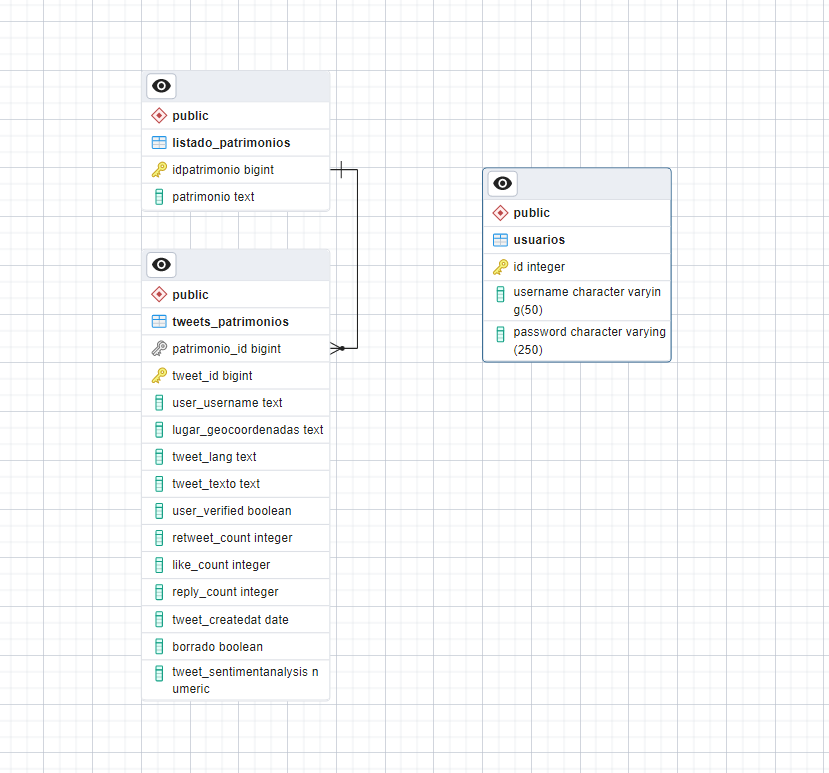
\includegraphics[scale=0.6]{img/TablasBD.PNG} 
    \caption{Diseño de datos - Estructura de base de datos}
     \label{Diseño de datos - Estructura de base de datos}
\end{figure}
Cada una de dichas tablas, a su vez, se descomponen en columnas con la información asociada. La organización que se ha decidido seguir es la siguiente:

\begin{itemize}
    \item \textbf{TABLA USUARIOS:} 
    \begin{enumerate}
        \item Id: número único e identificativo del usuario (en este caso del administrador).
        \item Usuario: usuario con el que se iniciará sesión como 'Administrador'.
        \item Contraseña: contraseña encriptada asociada al rol 'Administrador'.
    \end{enumerate}
    \item \textbf{TABLA LISTADO\_PATRIMONIOS:}  
    \begin{enumerate}
        \item id: número único e identificativo de cada BIC.
        \item Patrimonio: nombre de cada uno de los BICs de la etapa de Castilla y León.
    \end{enumerate}
    \item \textbf{TABLA TWEETS\_PATRIMONIOS:}  
    \begin{enumerate}

        \item Patrimonio\_Id: número único e identificativo de cada BIC que conecta la tabla Tweets\_Patrimonios con esta tabla.
        \item Tweet\_Id: número único e identificativo de cada tweet recopilado.
        \item Lugar\_GeoCoordenadas: identificación del lugar desde donde se publicó el tweet. Puede que no se especifique ubicación en el tweet, por lo que el parámetro se especificará por defecto como "No hay geolocalización".
        \item Tweet\_Lang: idioma en el que se escribe el tweet. Al tratarse de Bienes de Interés Cultural situados en España, se espera que la mayoría de tweets estén en español (es).
        \item Tweet\_Texto: contenido del tweet recopilado de la API.
        \item User\_Username: nombre del usuario que ha publicado el tweet.
        \item User\_Verified: parámetro en el que se indica si el usuario está verificado o no.
        \item Retweet\_Count: parámetro en el que se guarda el número de retweets que ha obtenido ese tweet.
        \item Like\_Count: parámetro en el que se guardará el número de likes que ha obtenido ese tweet.
        \item Reply\_Count: parámetro en el que se guardará el número de respuestas que ha obtenido ese tweet.
        \item Tweet\_CreatedAt: parámetro en el que se especifica la fecha en la que el tweet fue publicado.
        \item Borrado: parámetro no obtenido de la API de Twitter. El administrador, en la creación de la base de datos, especificará la fecha desde la que se requieren los tweets, en caso de que la fecha introducida sea posterior a la primera fecha que consta en la base de datos, los tweets anteriores -y por tanto no requeridos- marcarán este parámetro a 'False' para que en el caso de que después se necesiten no se tengan que realizar tantas consultas a la API y se agilice el proceso de búsqueda.
        \item Tweet\_SentimentAnalysis: valoración numérica entre 0 (negativo) y 1 (positivo) del sentimiento del contenido del tweet calculado con la librería \textit{"sentiment\_analysis\_spanish"}.
    \end{enumerate}
\end{itemize}

\subsection{Estructura de csv:}
El fichero csv ha sido utilizado para obtener parámetros como la localización, destinado al desarrollo del mapa de inicio. \\
Se ha ordenado de tal manera:
\begin{itemize}
   
    \item \textbf{CSV inventario\_01:}  
    En este csv se guarda toda la información recopilada de la Junta de Castilla y León para después hacer uso de ella a la hora de configurar el mapa de la página de inicio de la publicación.\\
    Los parámetros que contiene son: 
    \begin{enumerate}
        \item n: número único e identificativo de cada BIC.
        \item cod\_jcyl: código de ordenación de los BICs para la Junta de Castilla y León.
        \item provincia: provincia a la que pertenece el patrimonio.
        \item municipio: municipio al que pertenece el BIC.
        \item localidad: localidad a la que pertenece el BIC.
        \item denominación: nombre identificativo de cada uno de los BICs.  
        \item categoría: tipo de BIC (castillo, monumento, rollo de justicia...)
        \item latitud: latitud a la que se encuentra el BIC.
        \item longitud: longitud a la que se encuentra el BIC.
        \item altitud: altitud a la que se encuentra el BIC.
    \end{enumerate}
      
\end{itemize}

\section{Diseño procedimental}
En este anexo se muestran los diagramas de secuencia de la aplicación para realizar la explicación del funcionamiento interno de la misma.
\subsection{Visualización de estadísticas}
Se muestra el diagrama de secuencia en la ejecución de mostrar los gráficos estadísticos (Figura C.2).\\

\begin{figure}[h!]
    \centering
    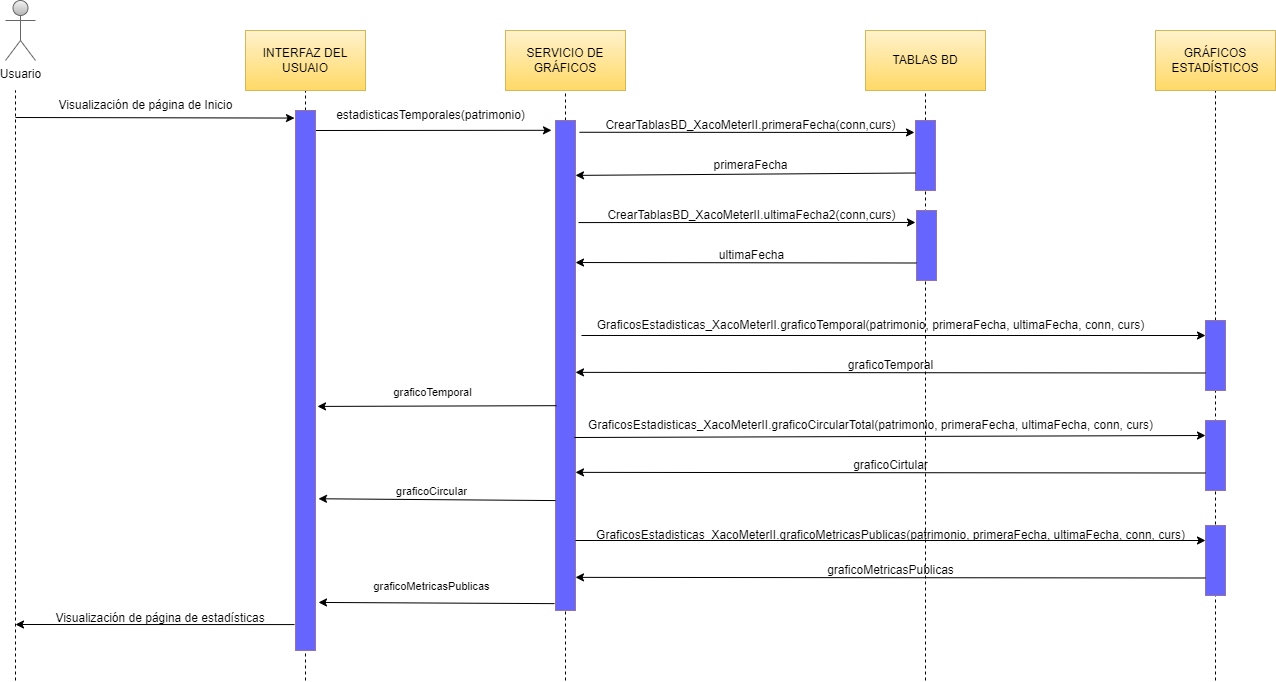
\includegraphics[scale=0.22]{img/DiagramaSecuencias_Estadisticas.png} \\
    \caption{Diagrama de secuencia - Estadísticas temporales}
    \label{Diagrama de secuencia - Estadísticas temporales}
\end{figure}

\subsection{Login}
Se muestra el diagrama de secuencia en la ejecución del inicio de sesión (Figura C.3).\\

\begin{figure}[h!]
    \centering
    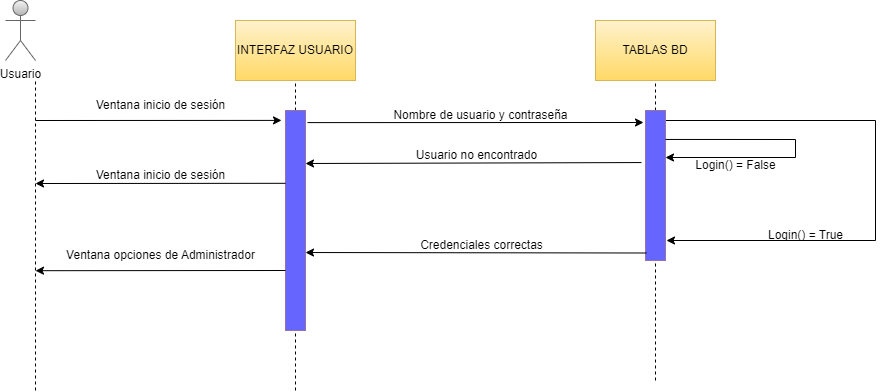
\includegraphics[scale=0.25]{img/DiagramaSecuencias_Login.png}\\
    \caption{Diagrama de secuencia - Inicio de sesión}
    \label{Diagrama de secuencia - Inicio de sesión}
\end{figure}


\subsection{Recopilación de datos}
Se muestra el diagrama de secuencia en la ejecución de recopilación de datos con la API y guardado en la base de datos (Figura C.4).\\


\begin{figure}[h!]
    \centering
    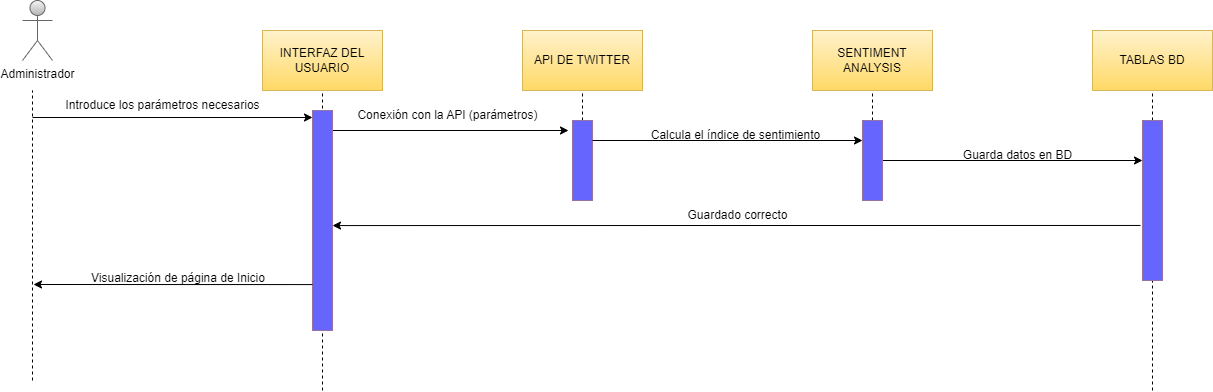
\includegraphics[scale=0.3]{img/DiagramaSecuencias_ActualizarCrear.png} \\
    \caption{Diagrama de secuencia - Creación de datos}
    \label{Diagrama de secuencia - Creación de datos}
\end{figure}



\section{Diseño arquitectónico}
En este apartado se explica el diseño que se ha seguido para desarrollar el proecto, pensado para contribuir a que la aplicación sea fácilmente escalable.


\subsection{Modelo-Vista-Controlador(MVC)}
El diseño Modelo-Vista-Controlador (Figura C.5), como describe su propio nombre, se basa en un patrón con tres componentes:
\begin{enumerate}
    \item \textbf{MODELO:}\\
    Es la lógica de los datos, es decir, el patrón que siguen los datos del programa.\\
    En XacoMeterII, el modelo está compuesto por la base de datos, la estructura del archivo csv y por la lógica que sigue la extracción de los datos de Twitter. 
    
    \item \textbf{VISTA:}\\
    La parte de la vista se refiere a la interfaz gráfica de la aplicación. \\
    En XacoMeterII, la vista está compuesta por todos los archivos \textit{.html} que contiene el proyecto, todos ellos agrupados en el directorio \textit{/templates}.
    
    \item \textbf{CONTROLADOR:}\\
    Es la parte del programa que manda realizar las operaciones, es decir, es el que se encarga de controlar cómo se mandan los datos y como recuperarlos. \\
    En XacoMeterII, el controlador está compuesto por el archivo \textit{main.py}.
    Además, el controlador cuenta con varios servicios que realizan las operaciones más complejas, que en el proyecto son todos los archivos .py incluido en el directorio \textit{/Code}.

\end{enumerate}

\begin{figure}[h!]
    \centering
    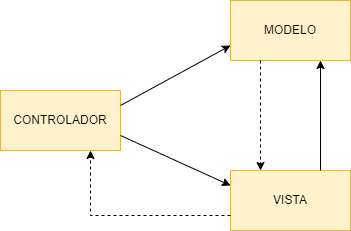
\includegraphics[scale=0.8]{img/MVC.png} \\
    \caption{Diseño arquitectónico - Modelo-Vista-Controlador}
    \label{Diseño arquitectónico - Modelo-Vista-Controlador}
\end{figure}

\subsection{Fachada \textit{(Facade)}}
El patrón fachada o \textit{"Facade"} es un patrón de diseño de software que proporciona una interfaz unificada sencilla que sirve de intermediaria entre los usuarios y el conjunto de interfaces en un subsistema.\cite{fachada}\\
Este patrón (Figura C.6), en este caso, se utiliza para simplificar la interfaz del usuario hacia un subsistema complejo, es decir, los módulos en los que se realizan las operaciones de conexión a la API de Twitter, creación de estadísticas, consultas a la base de datos... \\
En este caso, la fachada es el módulo \textit{main.py}, que comunica todos los módulos con el usuario, siendo así el intermediador.
\begin{figure}[h!]
    \centering
    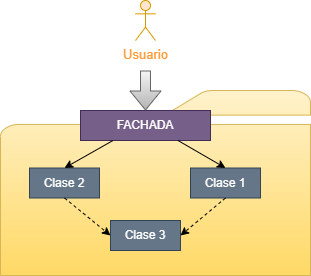
\includegraphics[scale=0.8]{img/patronFachada.png} \\
    \caption{Diseño arquitectónico - Fachada}
    \label{Diseño arquitectónico - Fachada}
\end{figure}

\apendice{Documentación técnica de programación}

\section{Introducción}
En este anexo, se describe la estructura del proyecto en directorios, la instalación del mismo y el proceso que se ha llevado a cabo para poder desplegarlo con Heroku.
\section{Estructura de directorios}
Se detalla a continuación la estructura que tiene el proyecto en en la organización de su código fuente, estando todo ello disponible en GitHub, excepto ciertos archivos que contienen información confidencial.
El directorio raíz \textit{'main'} se descompone en:
\begin{itemize}
    \item \textit{/Code:}\\
    Contiene los archivos \textit{.py} a los que llama la función principal \textit{'main'} para realizar todas las operaciones que necesite:
    \begin{itemize}
        \item Busqueda\_XacoMeterII.py:\\
        Contiene el diccionario desde el que se realizan las búsquedas con la API de Twitter.
        \item CrearTablasBD\_XacoMeterII.py:\\
        Contiene cada una de las operaciones que se van a realizar en la base de datos (UPDATE, SELECT...)
        \item Destinos\_XacoMeterII.py:\\
        Operaciones que realizan las llamadas a los archivos \textit{.py} que solicitan los datos a la API de Twitter y almacena la información en la base de datos.
        \item FunciónPrincipal\_XacoMeterII.py:\\
        Realiza la conexión con la API de Twitter y solicita la información requerida.
        \item GraficosEstadisticas\_XacoMeterII.py:\\
        Crea los gráficos, con la herramienta \textit{"Plotly"} de las estadísticas de los datos almacenados en la base de datos.
        \textit{"SentimentAnalysis\_XacoMeterII.py:}\\
        Realiza el cálculo del índice de sentimiento de los tweets almacenados de cada BIC.
    \end{itemize}
    \item \textit{/data:}\\
    Contiene los datos en formato csv.
    \begin{itemize}
        \item inventario\_01.csv:\\
        Este csv contiene todos los datos de los BICs según la organización que lleva la Junta de Castilla y León.
    \end{itemize}
    \item \textit{/static:}\\
    Contiene el archivo \textit{styles.css} el cual contiene contiene los estilos que se van a aplicar en la página web y las imágenes que se van a utilizar para mostrar en cada una de las páginas de la aplicación, por ejemplo, el logo de XacoMeterII.
    \item \textit{/templates:}\\
    Contiene todos los archivos \textit{.html} que definen la parte visual de la aplicación.
    \begin{itemize}
        \item admin\_Actualizar.html
        \item admin\_Crear.html
        \item administradorOpciones.html
        \item barraLateral.html
        \item base2.html
        \item home.html
        \item login.html
        \item serieTemporal.html
    \end{itemize}
    \item \textit{/venv:}\\
    Contiene un árbol de directorios con ejecutables en Python que indican que es un entorno virtual.
    \item \textit{.gitignore:}\\
    Fichero que contiene el nombre de los archivos ocultos para GitHub.
    \item \textit{.env:}\\
    Fichero sensible con las contraseñas necesarias para el desarrollo del proyecto. Este archivo estará oculto para GitHub.
    \item \textit{LICENSE:}\\
    Licencia de la aplicación
    \item \textit{errores.log:}\\
    Archivo en el que se guardan los errores generados por la aplicación web ejecutada en local durante su uso.
    \item \textit{Procfile:}\\
    Archivo que especifica cuál es el archivo principal de la aplicación para Heroku.
    \item \textit{README.md:}\\
    Archivo que contiene una breve descripción del proyecto y unos primeros pasos para su utilización.
    \item \textit{ejecutable.bat:}\\
    Archivo \textit{batch} que ejecuta los comandos necesarios para activar el entorno y ejecutar la aplicación web con el fin de no tener que usar Visual Code y poder ver la aplicación local en el navegador.
    \item \textit{main.py:}\\
    Archivo Python principal que realiza las llamadas a los demás archivos.
    \item \textit{requirements.txt:}\\
    Archivo que contiene un listado de las herramientas utilizadas -con sus versiones- para realizar el despliegue en Heroku.
    
\end{itemize}


\section{Manual del programador}
En este apartado se va a proceder a explicar los progrmas utilizados, su instalación y la razón de su uso.\\
El proyecto ha sido desarrollado de manera local en el equipo, se ha desplegado en Heroku y para la realización de pruebas en modo Administrador se dispondrá de una maquina virtual simulando el equipo local.\\
\subsection{Visual Studio Code}
Visual Studio Code se utiliza para realizar el desarrollo de la aplicación, la creación de archivos y métodos para el funcionamiento del proyecto.
Para la descarga de Visual Studio Code entramos en la página web \url{https://code.visualstudio.com/download} y seleccionamos, en nuestro caso, la versión para Windows (Figura D.1).\\
\begin{figure}[h!]
    \centering
    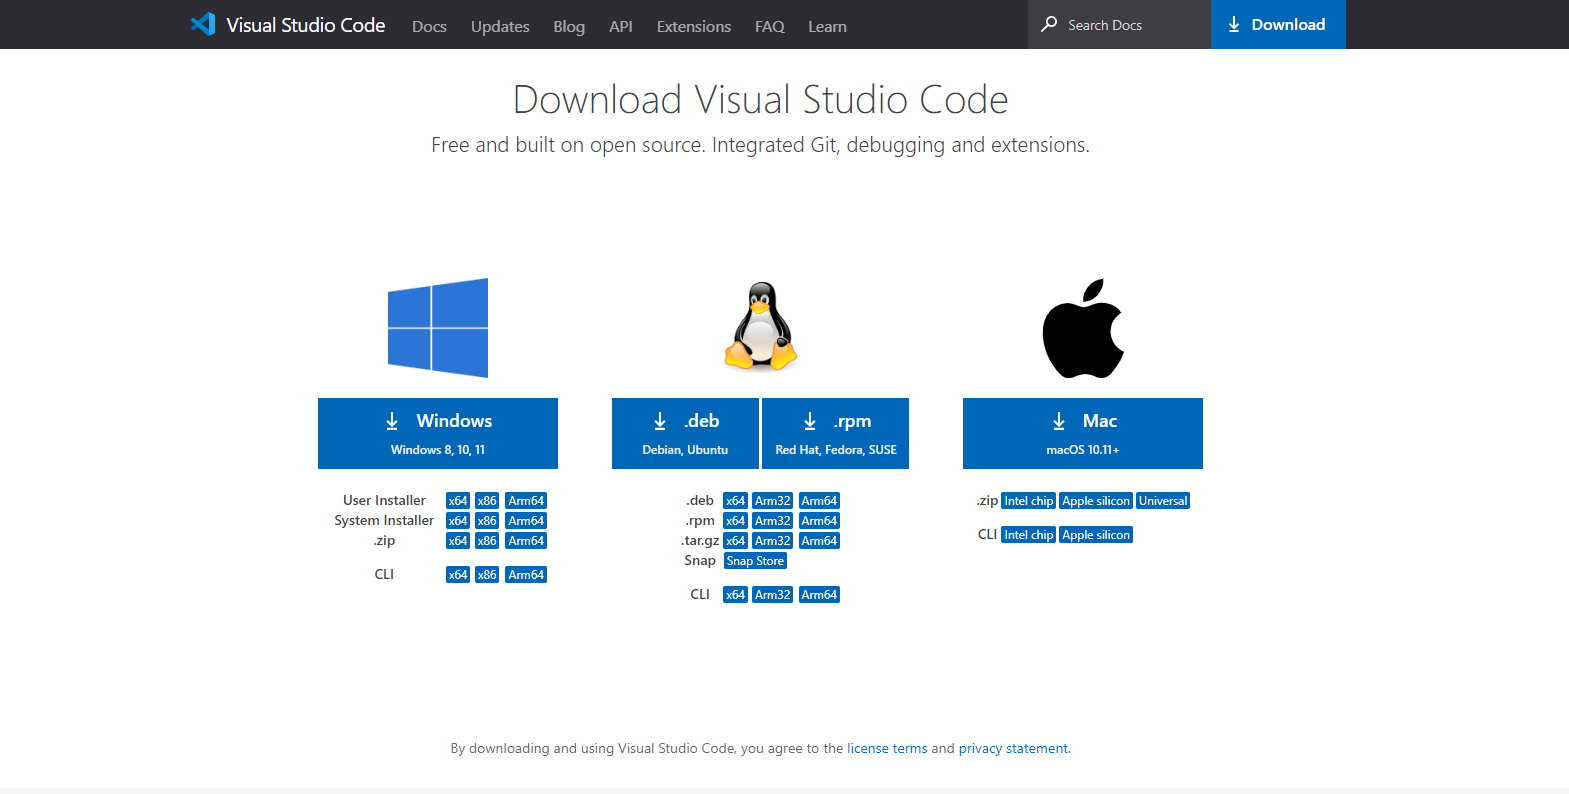
\includegraphics[scale=0.3]{img/VisualCode.png} \\
    \caption{Documentación del programador - Visual Studio Code}
    \label{Documentación del programador - Visual Studio Code}
\end{figure}
Una vez descargada la aplicación, debemos abrir el archivo de instalación \textit{.exe} para instalarlo y seguir los pasos hasta leer y aceptar el acuerdo de la licencia.
Una vez realizados los anteriores pasos, ya es posible empezar a trabajar con Visual Studio Code.
\subsection{PostgreSQL}
PostgreSQL es la base de datos que se ha decidido utilizar para la gestión de la base de datos, ya que puede ser desplegada en Heroku.\\
Para su descarga debemos entrar en la página \url{https://www.postgresql.org/download/} y pulsar sobre el icono de Windows. Una vez seleccionado Windows, debemos seleccionar la versión. Lo recomendable es utilizar la última versión, ya que siempre será la más actualizada, en este caso la versión 15 para Windows de 64-bit (Figura D.2). 
\begin{figure}[h!]
    \centering
    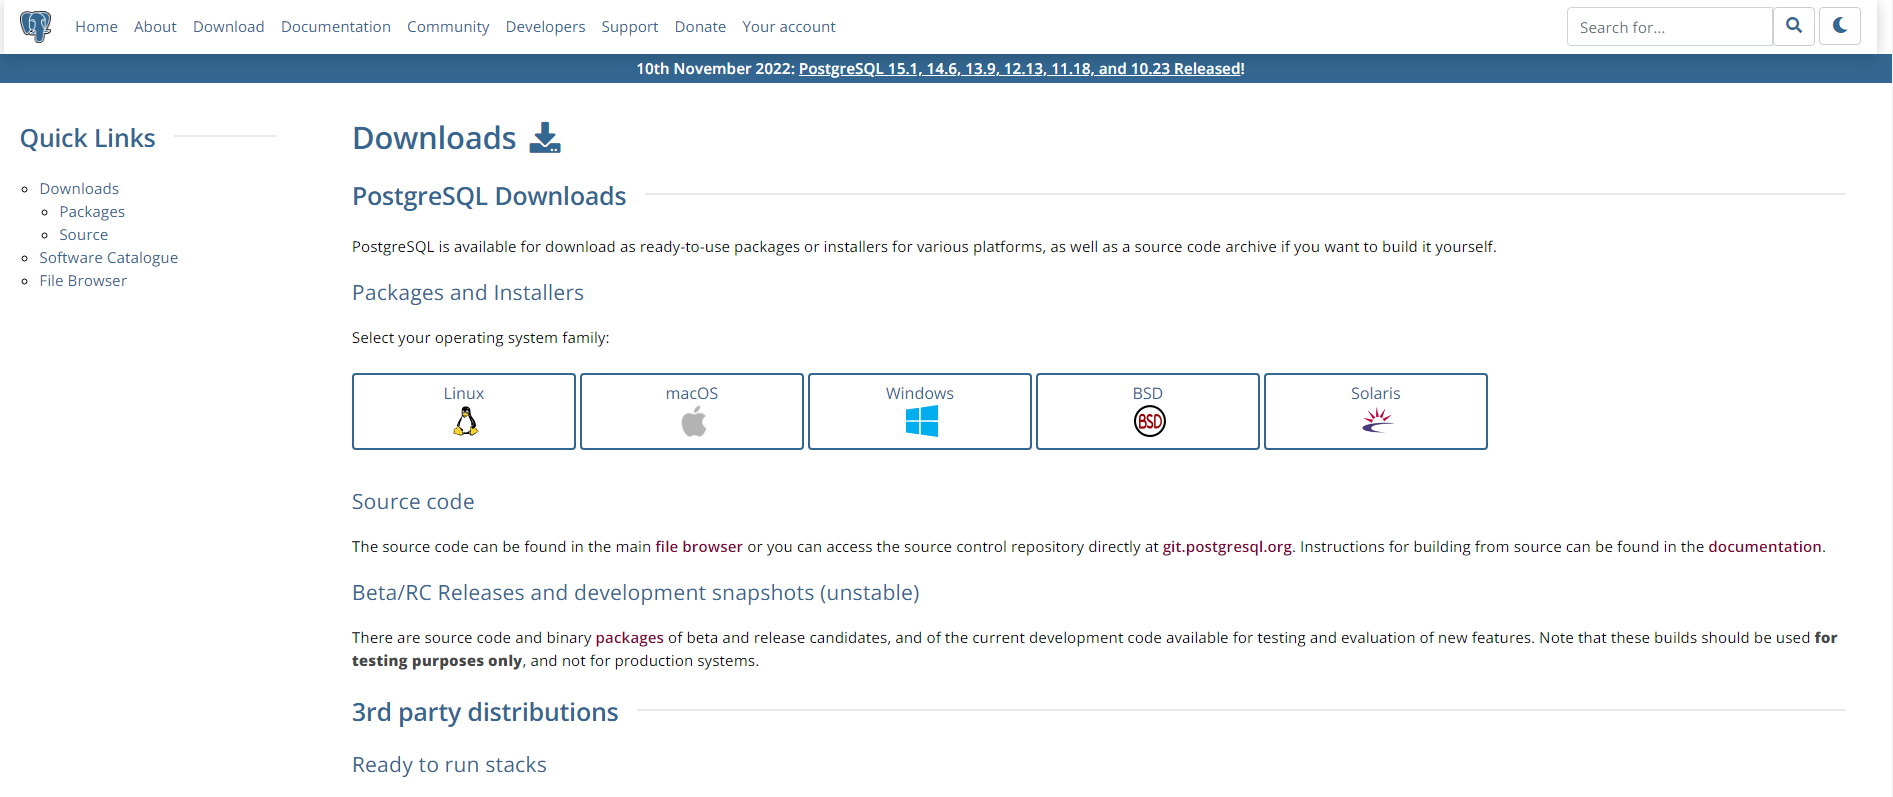
\includegraphics[scale=0.2]{img/postgreSQL.png}\\
    \caption{Documentación del programador - PostgreSQL}
    \label{Documentación del programador - PostgreSQL}
\end{figure}

Una vez que ha sido descargada, debemos busar el archivo \textit{.exe} y ejecutarlo para realizar la instalación.\\
Solamente se necesita continuar con todos los pasos y aceptar la licencia de PostreSQL.\\
Una vez tengamos todo instalado, hay que configurarlo para poder acceder a la base de datos de Heroku.\\
Para ello, creamos un nuevo servidor (Figura D.3):
\begin{figure}[h!]
    \centering
    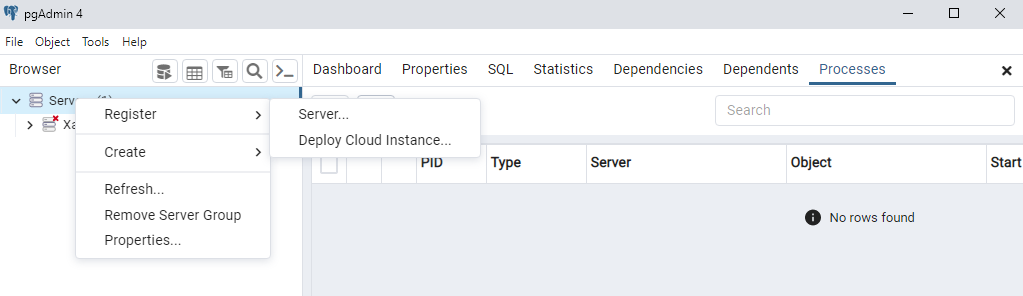
\includegraphics[scale=0.5]{img/nuevoServer.png}
    \caption{Documentación del programador - Crear servidor}
    \label{Documentación del programador - Crear servidor}
\end{figure}


Y realizamos la configuración con los datos que obtenemos del Add-on de Heroku (Figura D.4, Figura D.5, Figura D.6):\\
\begin{figure}[H]
    \hspace{0.2cm}
    \begin{minipage}[b]{0.3\linewidth}
        \centering
        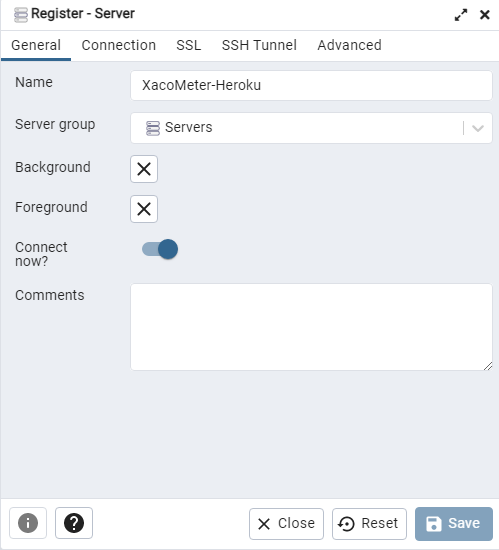
\includegraphics[scale=0.3]{img/GeneralPostgresql.png} \\
        \caption{Documentación del programador - pgAdmin4 general}
        \label{Documentación del programador - pgAdmin4 general}
    \end{minipage}
    \hspace{0.2cm}
    \begin{minipage}[b]{0.3\linewidth}
        \centering
        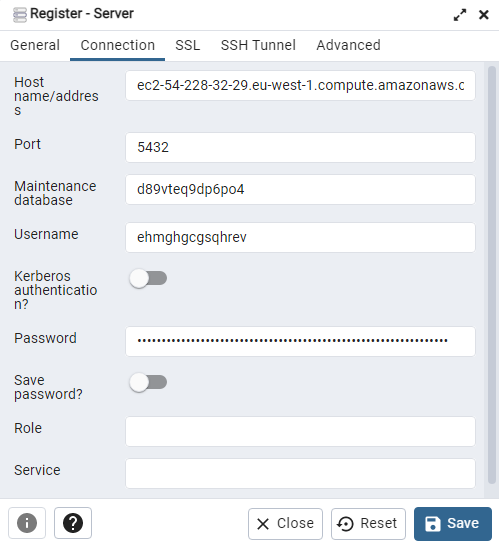
\includegraphics[scale=0.3]{ConnectionPostgresql.png}
        \caption{Documentación del programador - pgAdmin4 conexión}
        \label{Documentación del programador - pgAdmin4 conexión}
    \end{minipage}
    \hspace{0.2cm}
    \begin{minipage}[b]{0.3\linewidth}
        \centering
        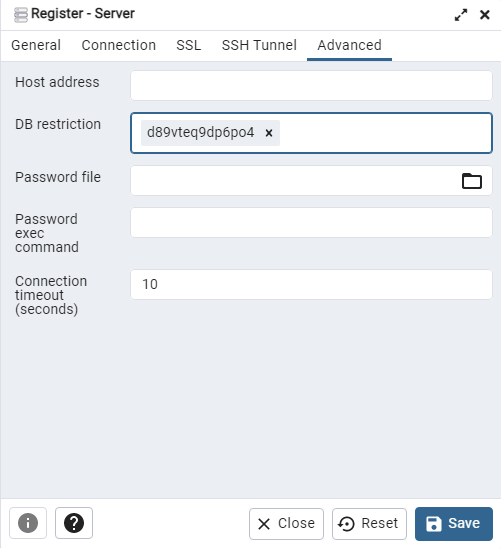
\includegraphics[scale=0.3]{AdvancedPostgresql.png}
        \caption{Documentación del programador - pgAdmin4 avanzado}
        \label{Documentación del programador - pgAdmin4 avanzado}
    \end{minipage}
\end{figure}
\subsection{Virtual Box}
En el caso de este proyecto vamos a elegir una máquina virtual para poder exportar el proyecto y que se puedan realizar pruebas en local del mismo, pudiendo así utilizar la función de Administrador, que por las limitaciones de Heroku, no permiten comprobar su funcionamiento.\\ Yo he decidido usar “VirtualBox” porque frente a otras
plataformas, como puede ser VMware, la interfaz de usuario es muy sencilla y además tiene
un mejor rendimiento, por lo que es más rápida y podemos utilizar las \textit{“guest additions”}
como tener carpetas compartidas con nuestro equipo o arrastrar y copiar del
portapapeles respecto al equipo anfitrión.\\
\begin{enumerate}
    \item \textbf{Instalación de VirtualBox:}
    Nos dirigimos a \url{www.virtualbox.org}, entramos en descargas y seleccionamos la versión
    que queremos y el paquete indicado para nuestro sistema operativo, Windows hosts (Figura D.7).
    Para instalarlo solo debemos seguir los pasos que se nos indican y al terminar pulsar el
    botón “FINISH”.
    \begin{figure}[h!]
        \centering
        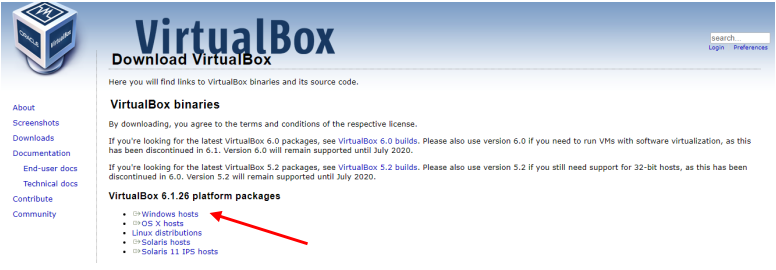
\includegraphics[scale=0.6]{img/DescargaVirtualBox.png} \\
        \caption{Documentación del programador - VirtualBox}
        \label{Documentación del programador - VirtualBox}
    \end{figure}
    \item \textbf{Instalación del sistema operativo:}
    En este caso, se va a utilizar Windows 10 Pro, con una licencia OEM que se ha comprado a través de RoyalCDKeys.\cite{RoyalCDKeys}\\
    Entramos en la página \url{https://www.microsoft.com/es-es/software-download/windows10} y, para poder decargar la ISO, solo hace falta dar a la tecla F12 para navegar como un desarrollador y elegir la última versión, ya que es la más actualizada, de Windows 10 de 64 bits y dar al botón descargar.\\
    Creamos una máquina dentro de VirtualBox pulsando en el botón de “nueva”. Ponemos el
    nombre que queremos para nuestra máquina virtual, en este caso XacoMeter\_NataliaFranco, y el sistema operativo que hemos decidido que vamos a instalar (Windows 10 64-bit). Le damos al botón \textit{Next} y nos dice que le indiquemos cuánta RAM queremos que tenga; este valor es mejor dejarlo como
    se nos recomienda, ya que si lo ampliamos, nos quitaría memoria de nuestro sistema
    operativo anfitrión (Windows). A continuación, creamos un disco duro VDI para almacenar el sistema
    operativo que le vamos a introducir y también, los archivos y programas (aproximadamente 25Gb
    es una cifra suficiente para trabajar con la máquina perfectamente).\\
    Para instalar Windows 10 en la máquina que hemos creado, vamos al botón de
    “Configuración”, a “Almacenamiento” y en “Controlador: IDE” añadimos una unidad
    óptica. Seleccionamos el archivo ISO que tenemos descargado y aceptamos (Figura D.8).
    \begin{figure}[h!]
        \centering
        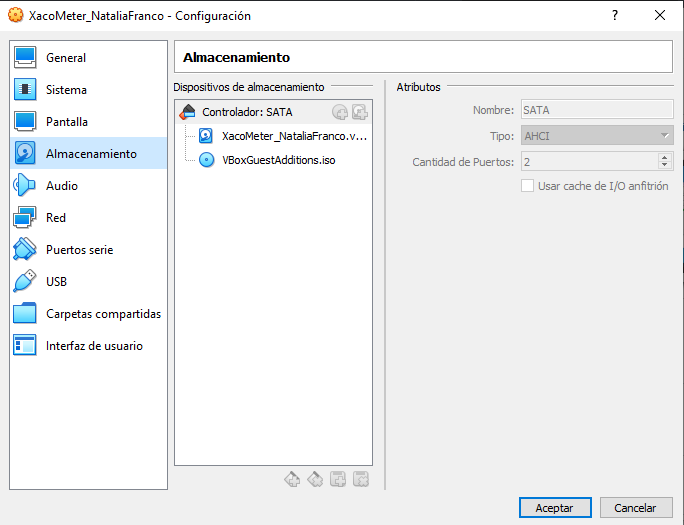
\includegraphics[scale=0.7]{img/ISO.png} \\
        \caption{Documentación del programador - Windows 10}
        \label{Documentación del programador - Windows 10}
    \end{figure}

    
    Al abrir la máquina nos aparecerá la instalación de Windows, introducimos la licencia que hemos comprado de Windows 10 Pro OEM y aceptamos los términos de la licencia.
    \item \textbf{Instalación de programas:}
    Una vez realizada la instalación, se deben seguir los pasos anteriormente descritos para la instalación de Visual Studio Code y pgAdmin4.\\
    Se importan los archivos a la máquina virtual para su uso y se configura la base de datos.\\
    Además, se descargará Google Chrome, donde se podrá ver la aplicación web y probarla.
    \item \textbf{Exportación de máquina virtual:}
    En VirtualBox, pulsar sobre "Archivo" y "Exportar servicio virtualizado". Solo hay que indicar la máquina virtual a exportar y el nombre con la extensión, en este caso, \textit{XacoMeter\_NataliaFranco.ova}.
\end{enumerate}
\section{Compilación, instalación y ejecución del proyecto}
La ejecución del proyecto se puede realizar de dos maneras, en función de las utilidades que se le vayan a dar. El proyecto puede ejecutarse bien en local, a través de la máquina virtual que se facilita o bien, a través de la página web desplegada en heroku.
\subsection{Ejecución en local}
Para la ejecución del proyecto en local, se facilita una máquina virtual de VirtualBox con el sistema operativo Windows 10 con Visual Studio Code y PostgreSQL instalado para la comodidad de los usuarios administradores.\\
Esta máquina se facilita ya que, debido a las restricciones de la API de Twitter y el tiempo de ejecución de ciertas operaciones del modo administrador, no podrán ser utilizadas en la página desplegada ya que se recibirá un \textit{timeout.}\\
El pin del usuario XacoMeter en Windows es: '1761'\\
Una vez se haya ingresado en la cuenta se debe abrir la aplicación de Visual Studio Code e introducir los siguientes comandos (Figura D.9):\\
\begin{itemize}
    \item Activar el entorno virtual: \\
    \textit{.venv\textbackslash{Scripts\textbackslash{activate}}}
    \item Compilar el proyecto:\\
    \textit{python main.py}
\end{itemize}
\begin{figure}[h!]
    \centering
    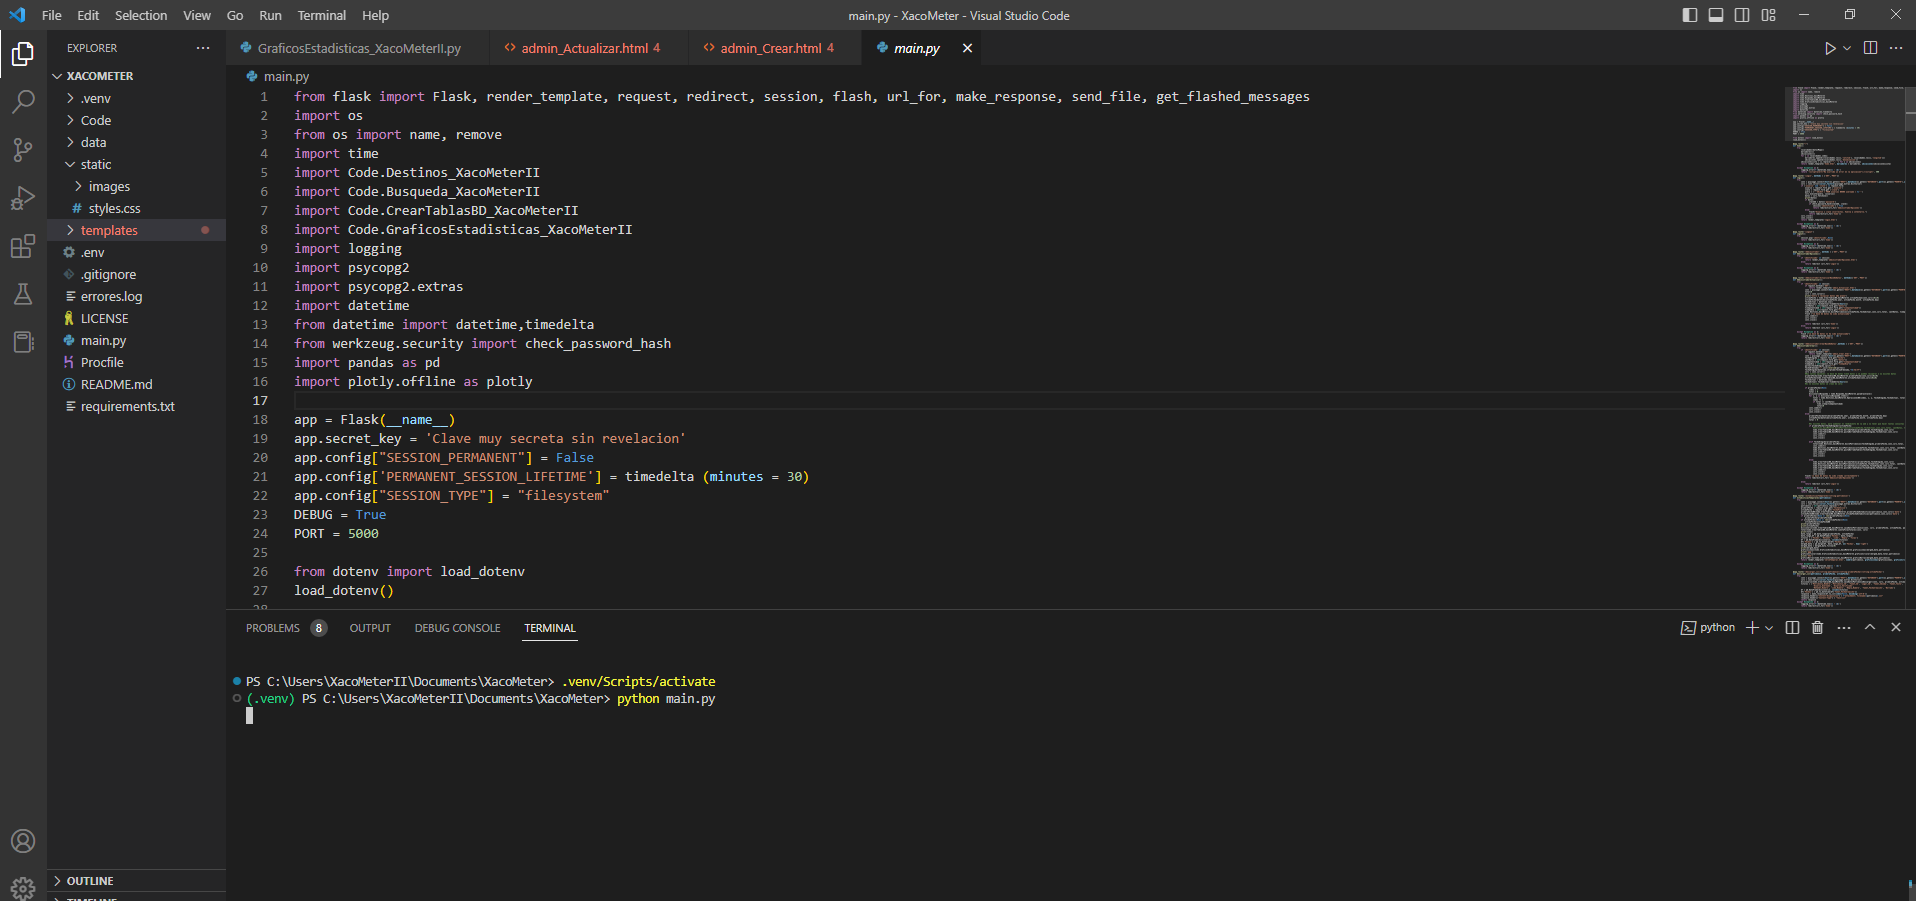
\includegraphics[scale=0.25]{img/Ejecutar.png} \\
    \caption{Documentación del programador - Comandos VS}
    \label{Documentación del programador - Comandos VS}
\end{figure}
También se ofrece la opción del uso del archivo \textit{ejecutable.bat}. Este es un archivo \textit{batch}, el cual, al hacer click sobre él, ejecuta los comandos que activan el entorno virtual y ejecutan el proyecto, lo cual permite que no se necesite abrir Visual Studio Code ni ejecutar comandos. Se ha creado un acceso directo en el escritorio de la máquina virtual del mismo para una mayor comodidad.\\

Para abrir la aplicación web se debe acceder desde el navegador (está instalado en la máquina virtual Microsoft Edge) a la URL \url{http://127.0.0.1:5000}.\\
Si se quieren visualizar las tablas de la base de datos, se necesita entrar en pgAdmin4 con el usuario: 'postgres' y la contraseña 'postgres'. Entrando en el servidor XacoMeter-Heroku, en la base de datos "d89vteq9dp6po4" con la contraseña "7b3278563bc4d86a321b8aab5716ef7b2e760978dfb4a23d8a392b36ea94d081" se podrán ejecutar las consultas deseadas con sql o ver las tablas en Schemas>public>Tables (Figura D.10).
\begin{figure}[h!]
        \centering
        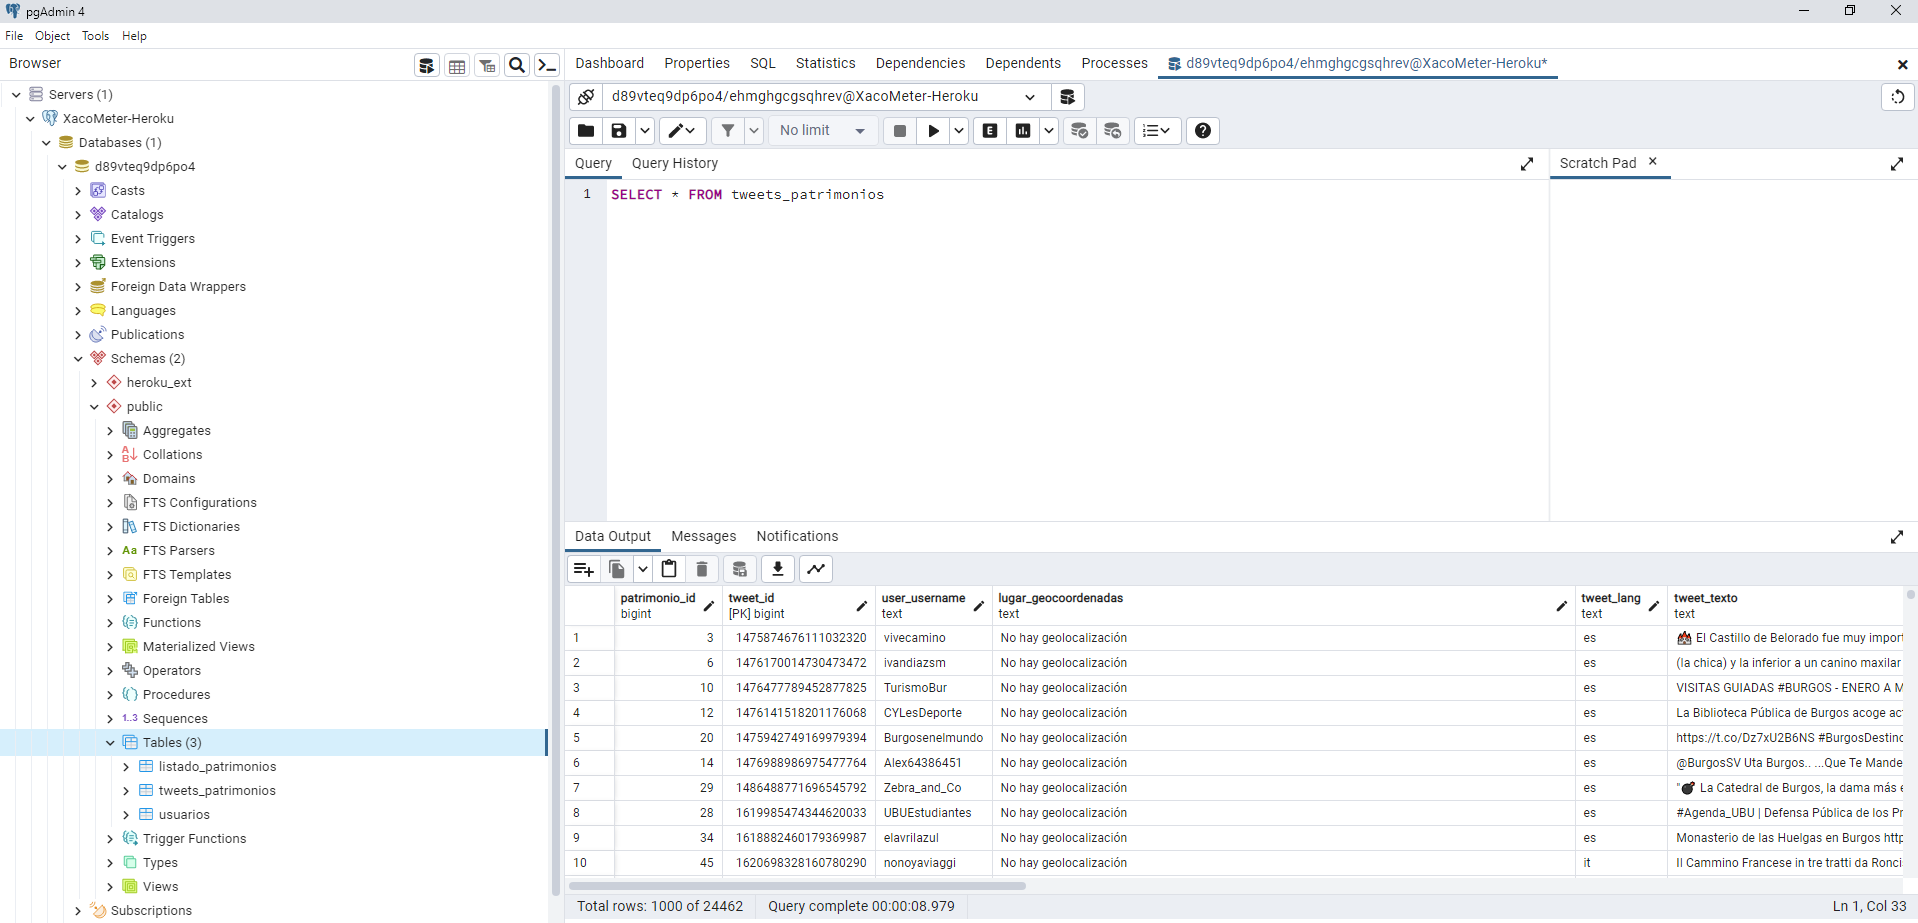
\includegraphics[scale=0.25]{img/pgAdmin4.png} \\
        \caption{Documentación del programador - pgAdmin 4}
        \label{Documentación del programador -pgAdmin 4}
    \end{figure}
\subsection{Despliegue en Heroku}
Para desplegar la aplicación en Heroku, al ser de pago, se debe conectar nuestra cuenta de GitHub con Heroku, ya que de esta manera, al ser estudiante, Heroku te permite obtener una cuantía de créditos suficientes para el despliegue del proyecto durante varios meses.\\
Deberemos crear una aplicación en Heroku indicando el nombre y la región de la aplicación que va a ser utilizada para localizar la página web (Figura D.11).
\begin{figure}[h!]
    \centering
    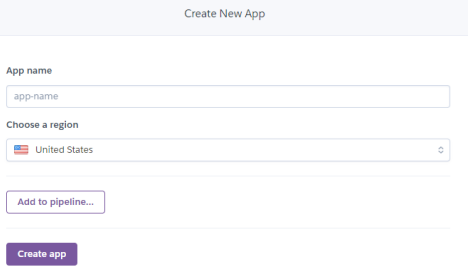
\includegraphics[scale=0.6]{img/CrearAPP.png} \\
    \caption{Documentación del programador - Heroku App}
    \label{Documentación del programador - Heroku App}
\end{figure}


Para el despliegue de la aplicación en Heroku, se necesita tener un archivo \textit{Procfile} que indique el comando a ejecutar en Heroku con el archivo principal, y también un archivo \textit{requirements} que contenga el nombre y la versión de todas las librerias necesarias para la ejecución del proyecto.\\
Para el despliegue de la base de datos en Heroku, se necesita activar un \textit{Add-On} de Heroku PostgreSQL (Figura D.12), que crea una base de datos en la nube con un usuario, una contraseña que te facilita Heroku.
\begin{figure}[h!]
    \centering
    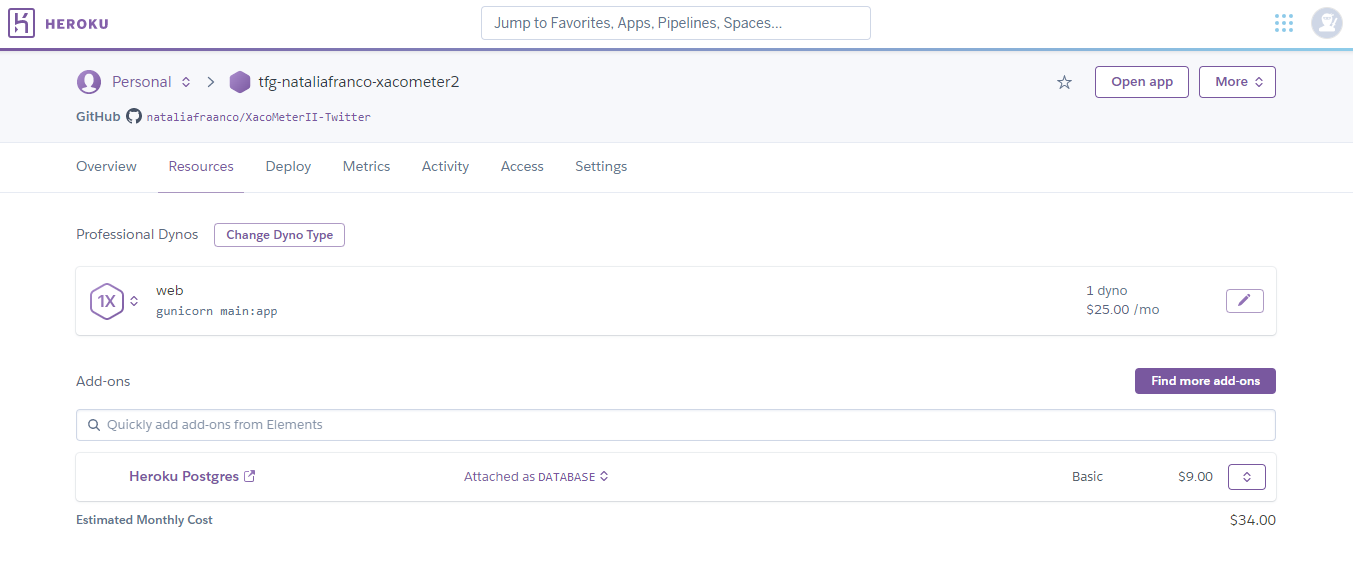
\includegraphics[scale=0.3]{img/Resources.png} \\
    \caption{Documentación del programador - Recursos}
    \label{Documentación del programador - Recursos}
\end{figure}


Para realizar el cambio de la base de datos local a la base de datos desplegada, tan solo se necesitará crear un \textit{backup}, o copia de seguridad, de la base de datos local y cargarla en la base de datos nueva de Heroku. Además, en el proyecto, para que se utilice la nueva base de datos desplegada, tan solo hará falta cambiar los parámetros de la base de datos en las variables de entorno guardadas en el archivo \textit{.env}.


Heroku, despliega la aplicación desde los archivos guardados en tu GitHub. En nuestro caso, como hay archivos como \textit{.env} que contienen información confidencial, como las contraseñas, estos no deben subirse a GitHub y deberán configurarse directamente en las variables de entorno de Heroku (Figura D.13):\\
\begin{figure}[h!]
    \centering
    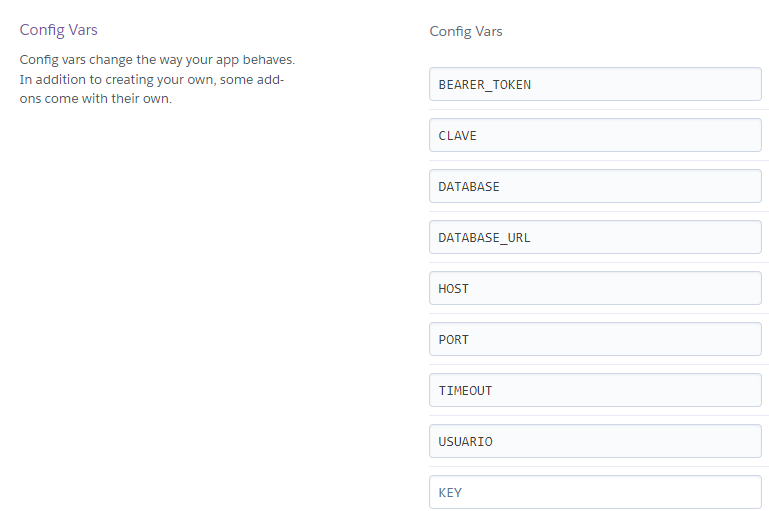
\includegraphics[scale=0.5]{img/ConfigVars.png} \\
    \caption{Documentación del programador - Configuración de variables}
    \label{Documentación del programador - Configuración de variables}
\end{figure}


Una vez hayamos configurado todo lo anterior, ya podremos desplegar el proyecto pulsando sobre \textit{'Deploy Branch'} (Figura D.14).
\begin{figure}[h!]
    \centering
    
\includegraphics[scale=0.5]{img/DeployBranch.png} \\
    \caption{Documentación del programador - Desplegar rama}
    \label{Documentación del programador - Desplegar rama}
\end{figure}
\section{Pruebas del sistema}
Como pruebas de la aplicación XacoMeterII, cabe destacar que se han realizado las siguientes:
\begin{enumerate}
    \item Comprobar que con los parámetros introducidos por defecto, la API de Twitter no deniega la generación de información.
    \item Poner decimales a los valores de los parámetros que deben ser enteros, no debe permitirlo.
    \item Probar el modo administrador con parámetros no permitidos para la API de Twitter.
    \item No introducir fecha de inicio en la creación de la base de datos.
    \item Introducir mal el usuario y contraseña del administrador para comprobar que no permite acceder.
    \item Introducir desde la URL las direcciones de actualizar y crear la base de datos para comprobar el correcto funcionamiento de denegar el acceso y redireccionar a la página de inicio de sesión.
    \item Comprobar que funcionan todas las redirecciones de los BICs en el inicio, tanto con el uso del mapa como del desplegable.
    \item Introducir en la página de estadísticas una fecha mayor de inicio que la fecha final, la aplicación debe mostrar que no hay datos entre esas fechas ya que siempre debe ser menor la fecha de inicio.
    \item Probar la funcionalidad de descarga del csv y que la importación en Excel puede realizarse correctamente mostrando todos los parámetros.
    \item Probar el funcionamiento de la barra navegadora.
    \item Probar el análisis de sentimientos.
    \item Introducir errores para visualizar mensajes de error.

\end{enumerate}
\apendice{Documentación de usuario}

\section{Introducción}
En este anexo se describirá el proceso que deben seguir los usuarios para la correcta utilización XacoMeterII.
\section{Requisitos de usuarios}
Se puede acceder a la aplicación XacoMeterII a través del enlace \url{https://tfg-nataliafranco-xacometer2.herokuapp.com/}.\\
La página ha sido desplegada a través de Heroku, pero debido a sus limitaciones de tiempo de espera y a las restricciones de la API de Twitter en cuanto a recopilación de datos, el modo \textit{Administrador} solo estará disponible para su uso en modo local. En caso de intentar acceder como administrador en la aplicación desplegada y solicitar crear la base de datos o actualizarla, la propia página generará un \textit{'timeout'}.\\
Para poder utilizar todas las funciones, incluyendo el modo \textit{'Administrador'}, se facilita una máquina virtual con todos los recursos instalados y puesta en marcha para funcionar en su totalidad, de esta manera no se tendrán limitaciones, excepto las marcadas por la API de Twitter.\\
Al ser una aplicación web se requiere acceso a internet y un navegador, o en el caso de utilizar el modo \textit{Administrador}, se requiere de la descarga de la máquina virtual.
\section{Instalación}
Los usuarios no necesitan instalar nada en el equipo para el uso de XacoMeterII, ya que se accede con un navegador web a través de internet.\\
En el caso de utilizar el modo \textit{'Administrador'} se dispone de una máquina virtual.

\section{Manual del usuario}
A continuación, se detallan los pasos a seguir para el correcto uso de la aplicación.
\subsection{Inicio}
Para iniciar la aplicación se accede a \url{https://tfg-nataliafranco-xacometer2.herokuapp.com/} en un navegador web.
Una vez se accede a la página web, lo primero que se visualiza es una página de inicio, en la que se puede ver un mapa dinámico con los Bienes de Interés Cultural del Camino de Santiago Francés en Castilla y León situados en él, una barra navegadora y un desplegable con el nombre de los BICs (Figura E.1).\\
\begin{figure}[h!]
    \centering
    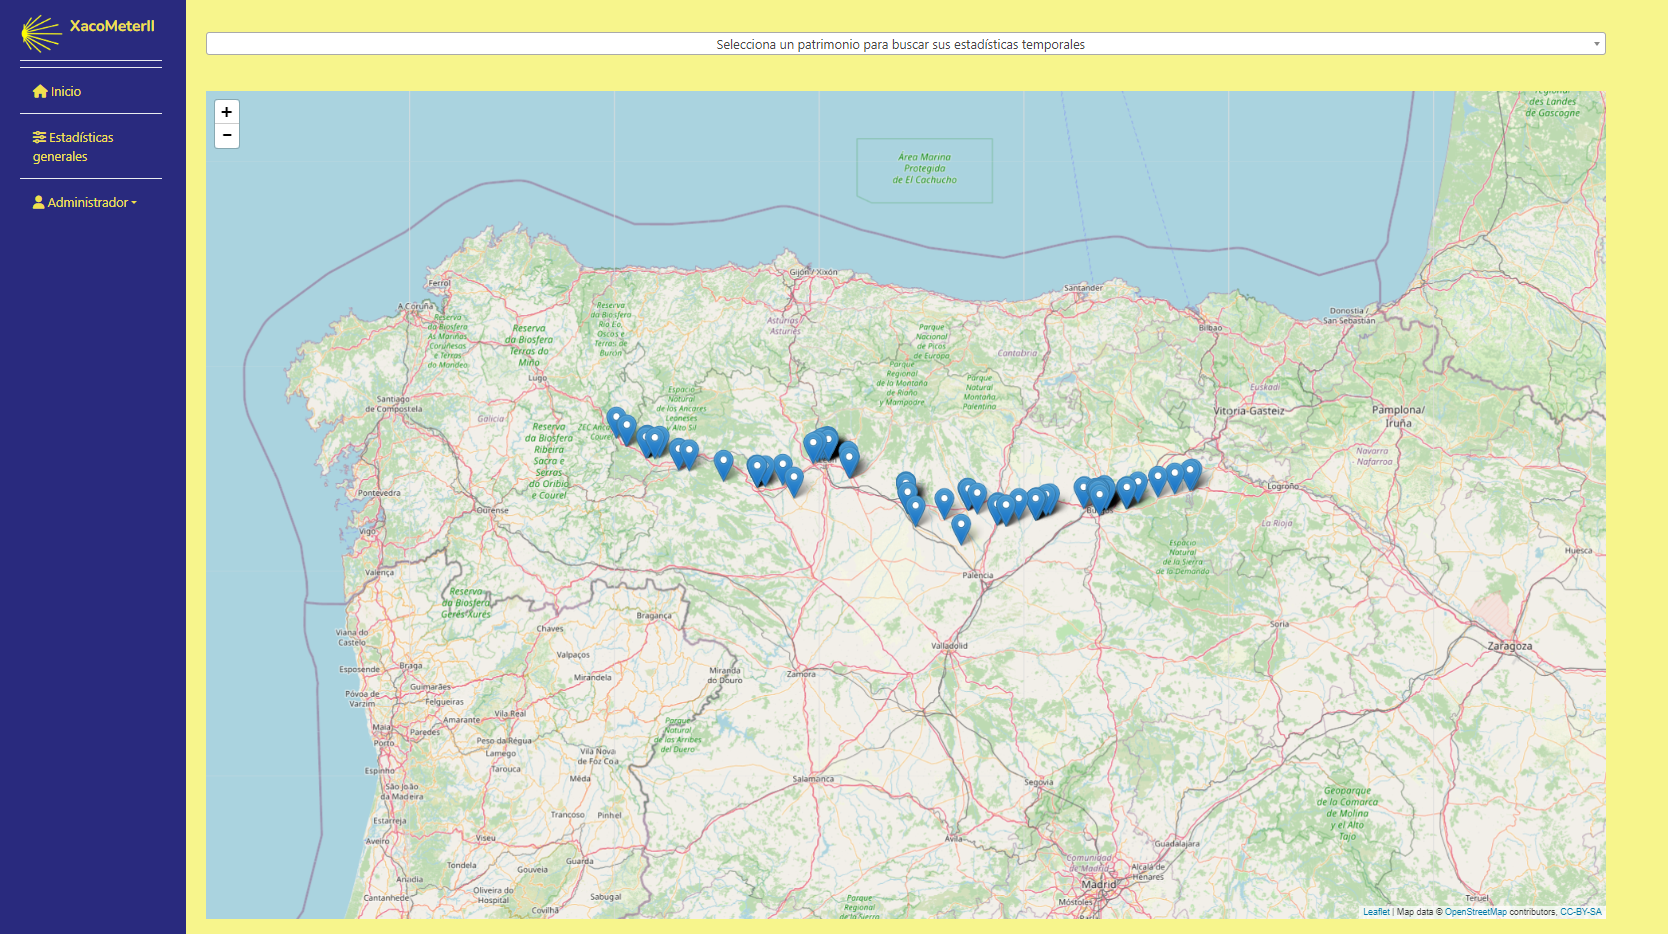
\includegraphics[scale=0.3]{img/Inicio.png} \\
    \caption{Documentación de usuario - Inicio}
    \label{Documentación de usuario - Inicio}
\end{figure}
\subsection{Barra navegadora}
Este elemento va a estar disponible en todas las páginas de la aplicación y va a permitir realizar las diferentes acciones posibles (Figura E.2, Figura E.3).\\
Además, se divide en dos secciones, según los permisos del usuario.\\
El botón \textbf{INICIO}, será un botón que puedan acceder todos los usuarios, con el que se redireccionará al usuario a la página de inicio.\\
El botón \textbf{ESTADÍSTICAS GENERALES}, será un botón que puedan acceder todos los usuarios, con el que se redireccionará al usuario a la página de estadísticas generales de todos los BICs.\\
El botón \textbf{ADMINISTRADOR} solo estará disponible para los usuarios en modo administrador y se podrá acceder tanto al inicio de sesión como a las opciones de administrador y además, permitirá cerrar sesión, todo ello contando con que el usuario ha introducido las credenciales correctamente.

\begin{figure}[H]
    \begin{minipage}[b]{0.5\linewidth}
        \centering
        
\includegraphics[scale=0.7]{img/BarraComprimida.png} \\
        \caption{Documentación de usuario - Barra de navegación comprimida}
        \label{Documentación de usuario - Barra de navegación comprimida}
    \end{minipage}
    \hspace{0.5cm}
    \begin{minipage}[b]{0.5\linewidth}
        \centering
        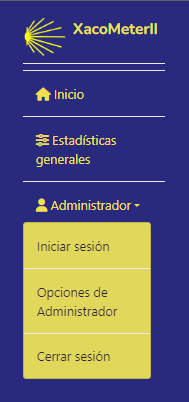
\includegraphics[scale=0.7]{BarraDesplegada.png}
        \caption{Documentación de usuario - Barra de navegación desplegada}
        \label{Documentación de usuario - Barra de navegación desplegada}
    \end{minipage}
\end{figure}

\subsection{Selección del patrimonio}
En la ventana de inicio se puede seleccionar un BIC para ser redirigido a la página de estadísticas temporales del mismo.\\
Esto se puede realizar de dos maneras:
\begin{enumerate}
    \item Utilizando el mapa dinámico (Figura E.4), con el que el usuario puede moverse con el ratón y seleccionar el BIC que desee.
    \begin{figure}[h!]
        \centering
        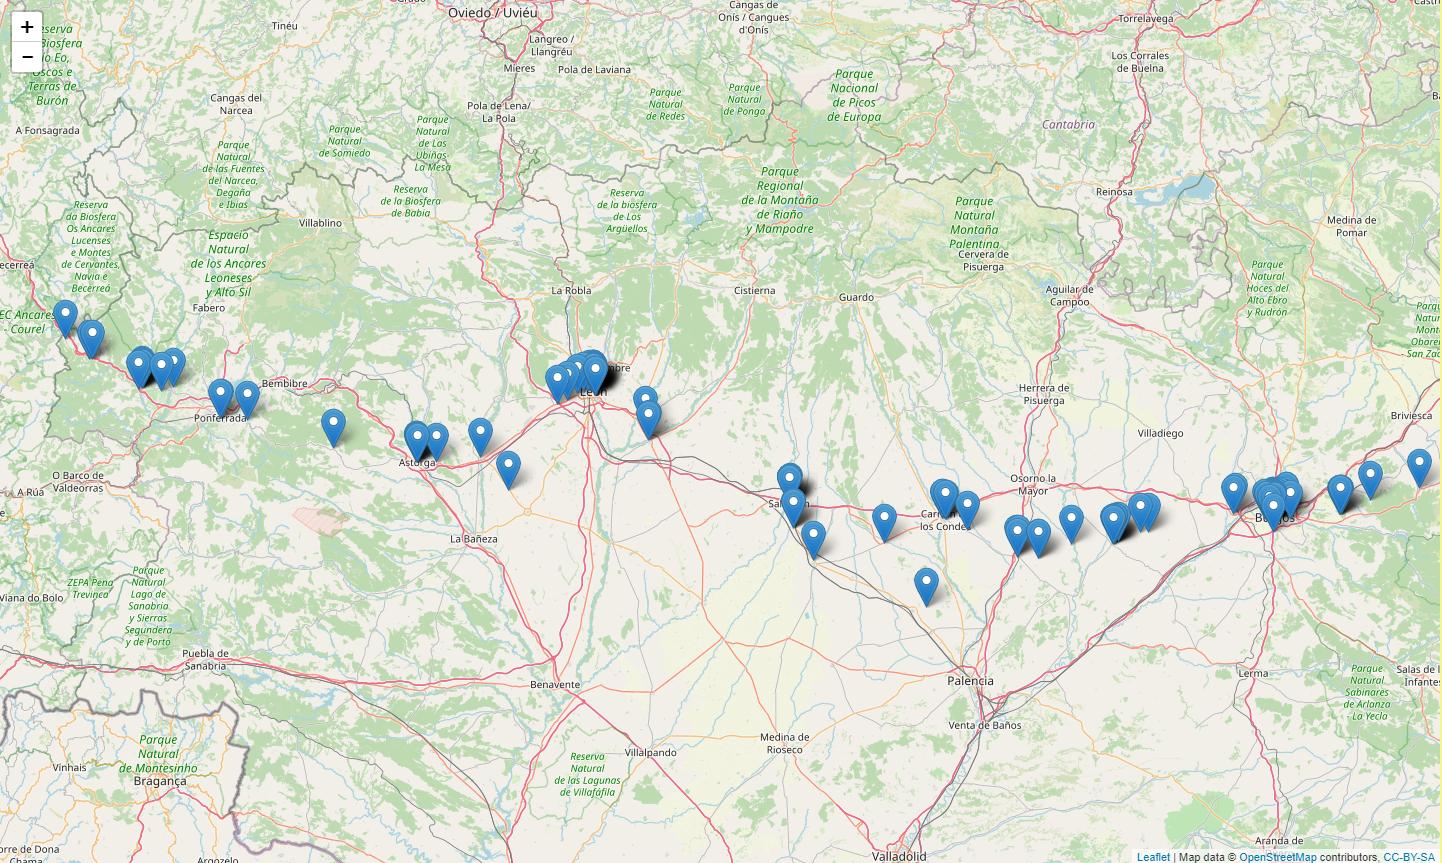
\includegraphics[scale=0.3]{img/Mapa.png} \\
        \caption{Documentación de usuario - Mapa}
        \label{Documentación de usuario - Mapa}
    \end{figure}
    \item Abriendo el desplegable que está situado encima del mapa y seleccionando un BIC (Figura E.5).
    \begin{figure}[h!]
        \centering
        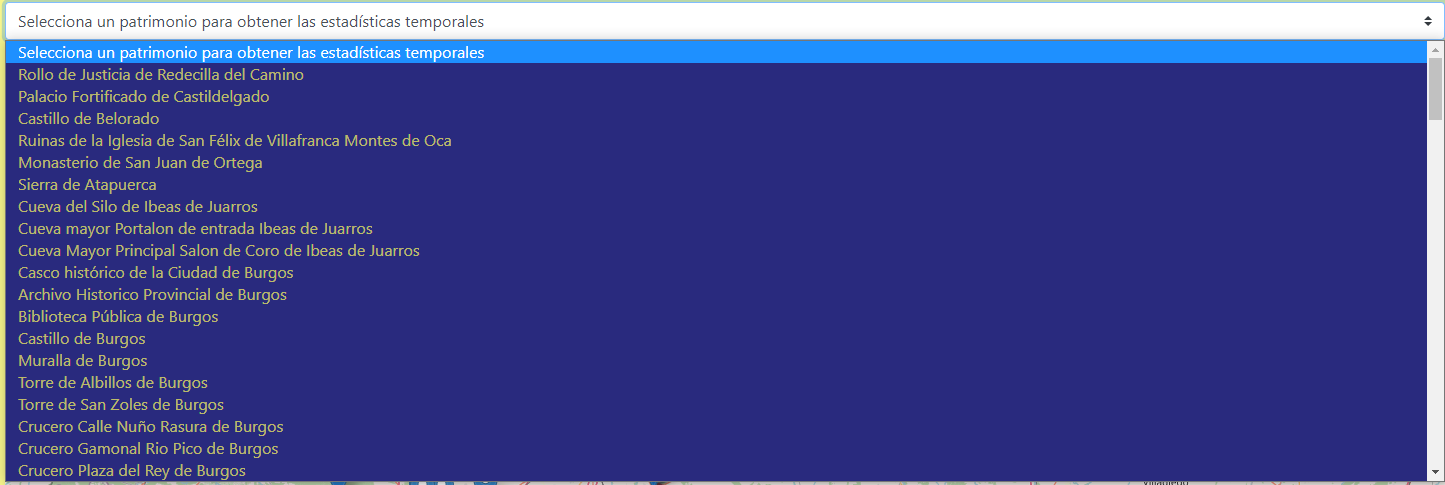
\includegraphics[scale=0.3]{img/DesplegablePatrimonios.png} \\
        \caption{Documentación de usuario - Desplegable patrimonios}
        \label{Documentación de usuario - Desplegable patrimonios}
    \end{figure}
\end{enumerate}
\subsection{Página de estadísticas temporales}
Una vez se ha seleccionado un BIC en la página de inicio, se redireccionará al usuario a la página de estadísticas temporales, en la que se mostrarán las estadísticas temporales del BIC entre las fechas existentes en la base de datos y el análisis de sentimientos (Figura E.6).\\
Esta página permite modificar las fechas de inicio y fin de las estadísticas, teniendo en cuenta que la fecha de inicio debe ser anterior que la fecha de fin.
Además esta página permite volver a la página de inicio y descargar el csv con los datos del patrimonio.
\begin{figure}[h!]
    \centering
    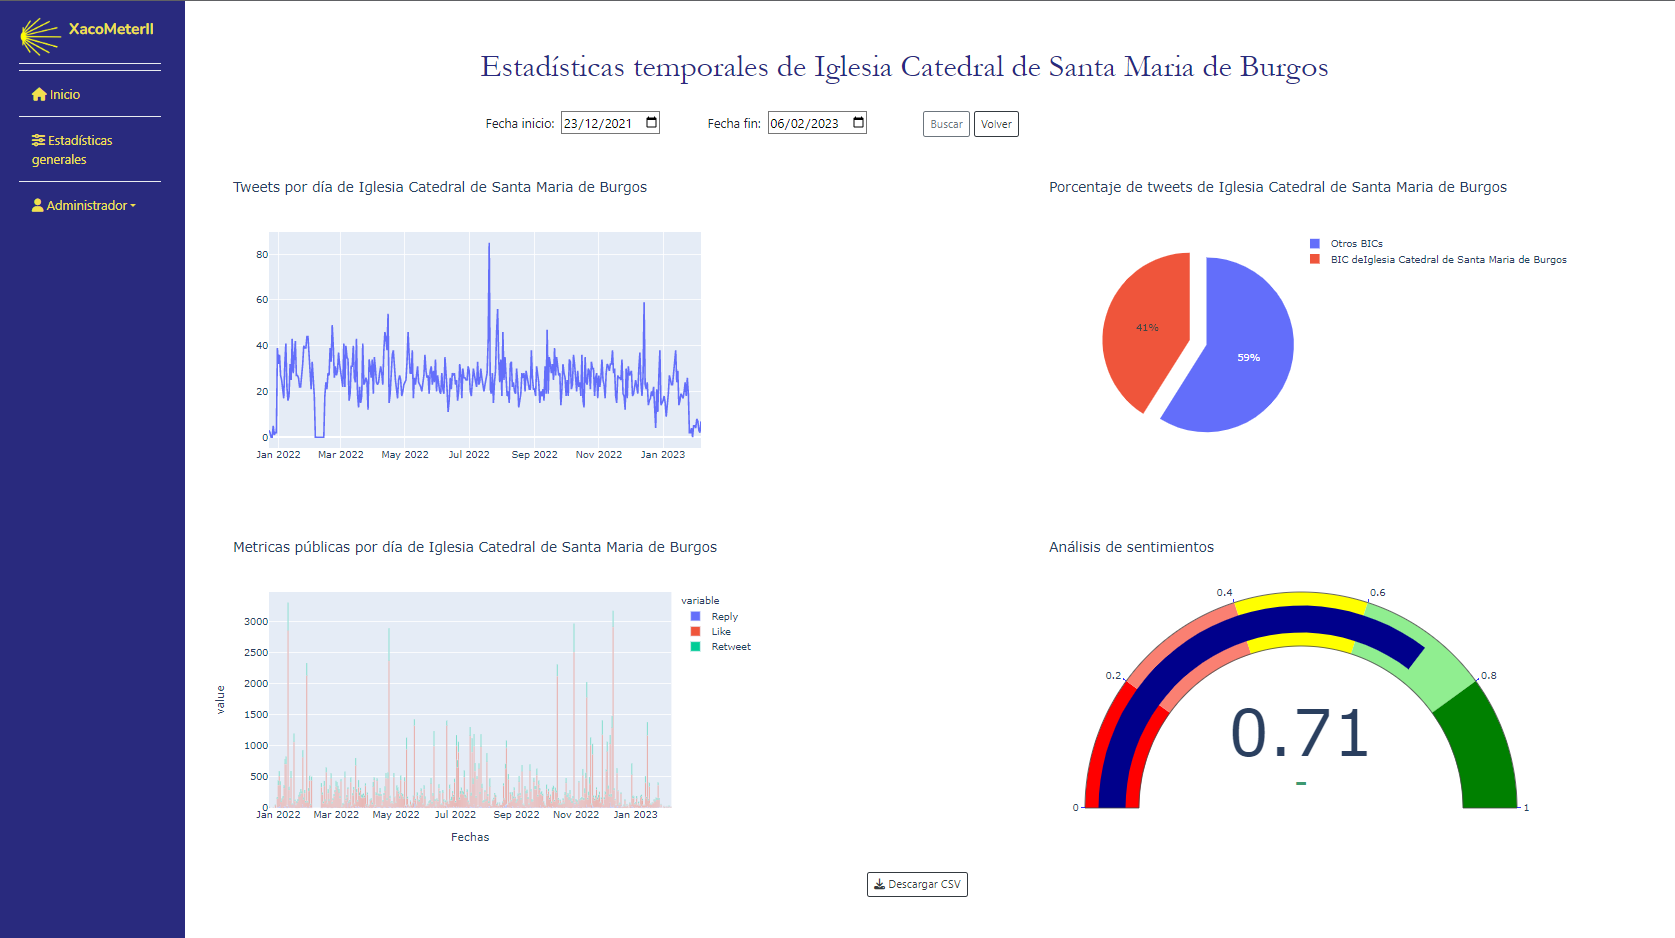
\includegraphics[scale=0.25]{img/Mejoras.png} 
    \caption{Documentación de usuario - Estadísticas temporales}
    \label{Documentación de usuario - Estadísticas temporales}
\end{figure}
\subsection{Gráfico de tweets por día}
Es el primer gráfico que se muestra en la página de estadísticas temporales. Muestra los tweets que se diariamente de este BIC en el periodo de tiempo establecido (Figura E.7).\\
Este gráfico es dinámico y se puede descargar en formato \textit{.PNG}, así como también se puede mover, ampliar y visualizar los datos de cada uno de sus puntos al poner el ratón sobre ellos.
\begin{figure}[h!]
    \centering
    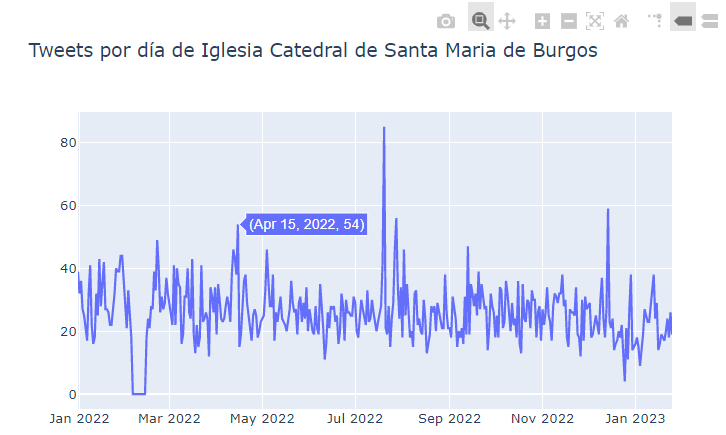
\includegraphics[scale=0.4]{img/TweetsDia.png} \\
    \caption{Documentación de usuario - Gráfico de tweets por día}
    \label{Documentación de usuario - Gráfico de tweets por día}
\end{figure}
\subsection{Gráfico de porcentaje de tweets}
En el segundo gráfico que se muestra en la página de estadísticas temporales, se puede ver el diagrama circular que muestra el porcentaje de tweets del BIC en cuestión con respecto al total de tweets (Figura E.8).\\
Este gráfico permite saber cuántos tweets totales tiene cada uno de los sectores poniendo el ratón sobre cada uno de ellos. También es posible descargar el gráfico en formato \textbf{.PNG}.\\
\begin{figure}[h!]
    \centering
    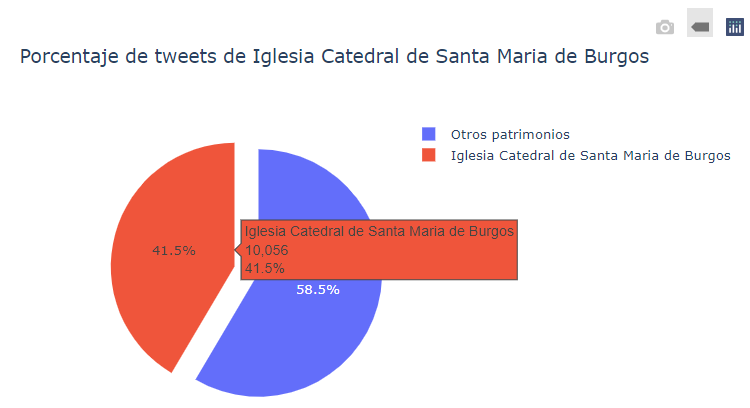
\includegraphics[scale=0.35]{img/TweetsPorcentaje.png} \\
    \caption{Documentación de usuario - Gráfico de porcentaje de tweets}
    \label{Documentación de usuario - Gráfico de porcentaje de tweets}
\end{figure}
\subsection{Gráfico de métricas públicas}
En el gráfico inferior de la página de estadísticas temporales, se pueden comparar las métricas públicas de cada BIC en el periodo temporal seleccionado. En este gráfico se utilizan los parámetros de \textit{likes, retweets y replies} que han tenido en un día los tweets publicados sobre ese BIC (Figura E.9).\\
Este gráfico permite realizar las mismas acciones que el gráfico de tweets por día, añadiendo la opción de seleccionar libremente un conjunto de datos del gráfico.
\begin{figure}[h!]
    \centering
    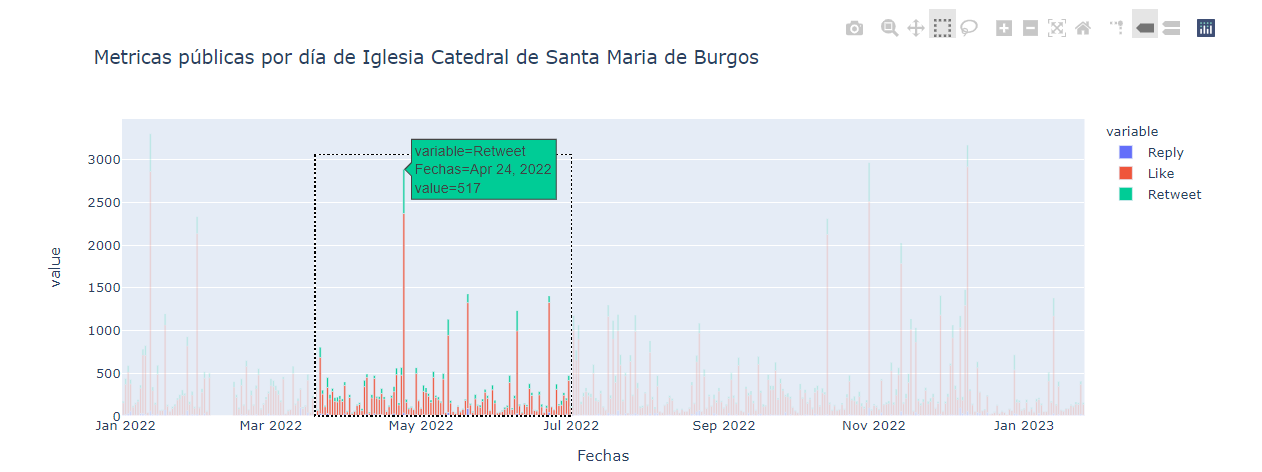
\includegraphics[scale=0.3]{img/MetricasPublicas.png} \\
    \caption{Documentación de usuario - Gráfico de métricas públicas}
    \label{Documentación de usuario - Gráfico de métricas públicas}
\end{figure}


\subsection{Gráfico de análisis de sentimientos}
En el cuarto gráfico de la página de estadísticas temporales se muestra en un diagrama semicircular del 0 (negativo) al 1 (positivo) el índice medio de sentimiento de los tweets del BIC seleccionado en el periodo temporal elegido (Figura E.10). \\
Este gráfico también muestra el número exacto del índice medio de sentimiento obtenido del BIC entre las fechas seleccionadas.\\
\begin{figure}[h!]
    \centering
    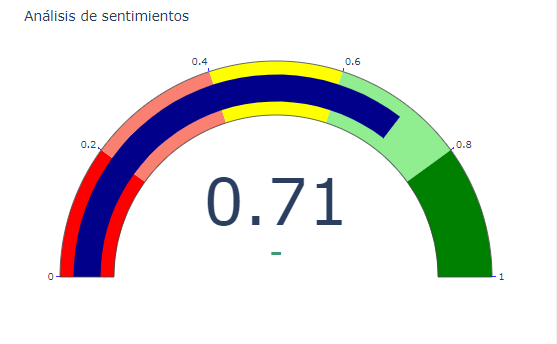
\includegraphics[scale=0.5]{img/AnalisisSentimientos.png} \\
    \caption{Documentación de usuario - Análisis de sentimientos}
    \label{Documentación de usuario - Análisis de sentimientos}
\end{figure}
\subsection{Descarga de datos}
Además, en la página de estadísticas temporales, se incluye un botón (Figura E.11) que, al pulsar en él, descarga un fichero \textit{.csv} (Figura E.12), que puede ser importado a Excel, en el que se muestran todos los tweets con sus parámetros por columnas.
\begin{figure}[H]
    \begin{minipage}[b]{0.5\linewidth}
        \centering
        
\includegraphics[scale=0.6]{img/Descarga.png} 
        \caption{Documentación de usuario - Botón descargar}
        \label{Documentación de usuario - Botón descargar}
    \end{minipage}
    \hspace{0.4cm}
    \begin{minipage}[b]{0.5\linewidth}
        \centering
        
\includegraphics[scale=0.55]{Descargacsv.png}
        \caption{Documentación de usuario - Descarga de .csv}
        \label{Documentación de usuario - Descarga de .csv}
    \end{minipage}
\end{figure}
La visualización de los datos puede realizarse de la siguiente manera:\\
\begin{enumerate}
    \item Entrar en Excel.
    \item Crear una hoja en blanco.
    \item Ir a la pestaña de datos y pulsar sobre \textbf{importar csv}.
    \item Se abrirá una pestaña con las opciones del csv (Figura E.13).
    \begin{figure}[h!]
        \centering
        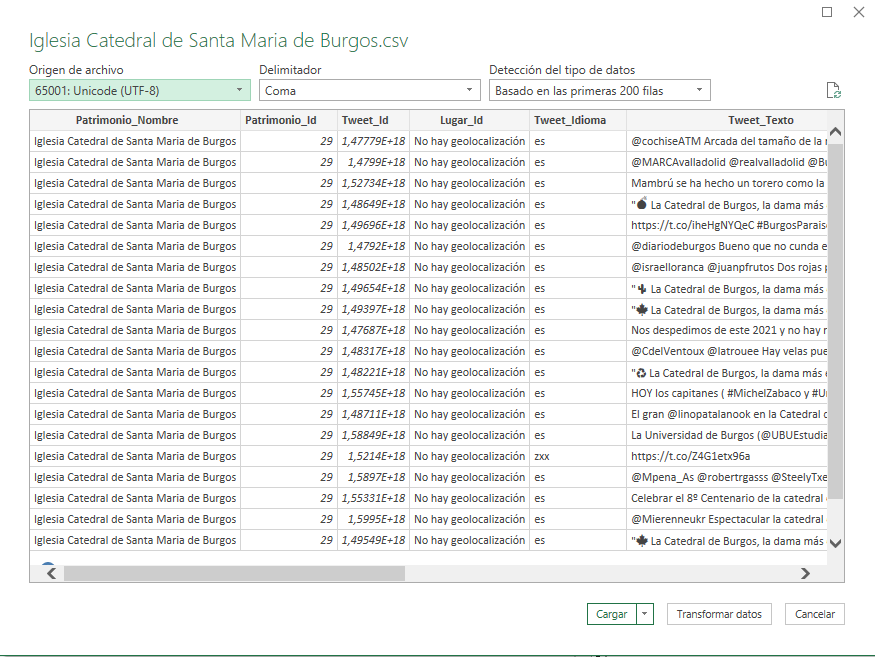
\includegraphics[scale=0.45]{img/ProcesoExcel.png} \\
        \caption{Documentación de usuario - Importar csv}
        \label{Documentación de usuario - Importar csv}
\end{figure}
    \item Dar al botón \textbf{cargar} (Figura E.14).
\end{enumerate}
\begin{figure}[h!]
    \centering
    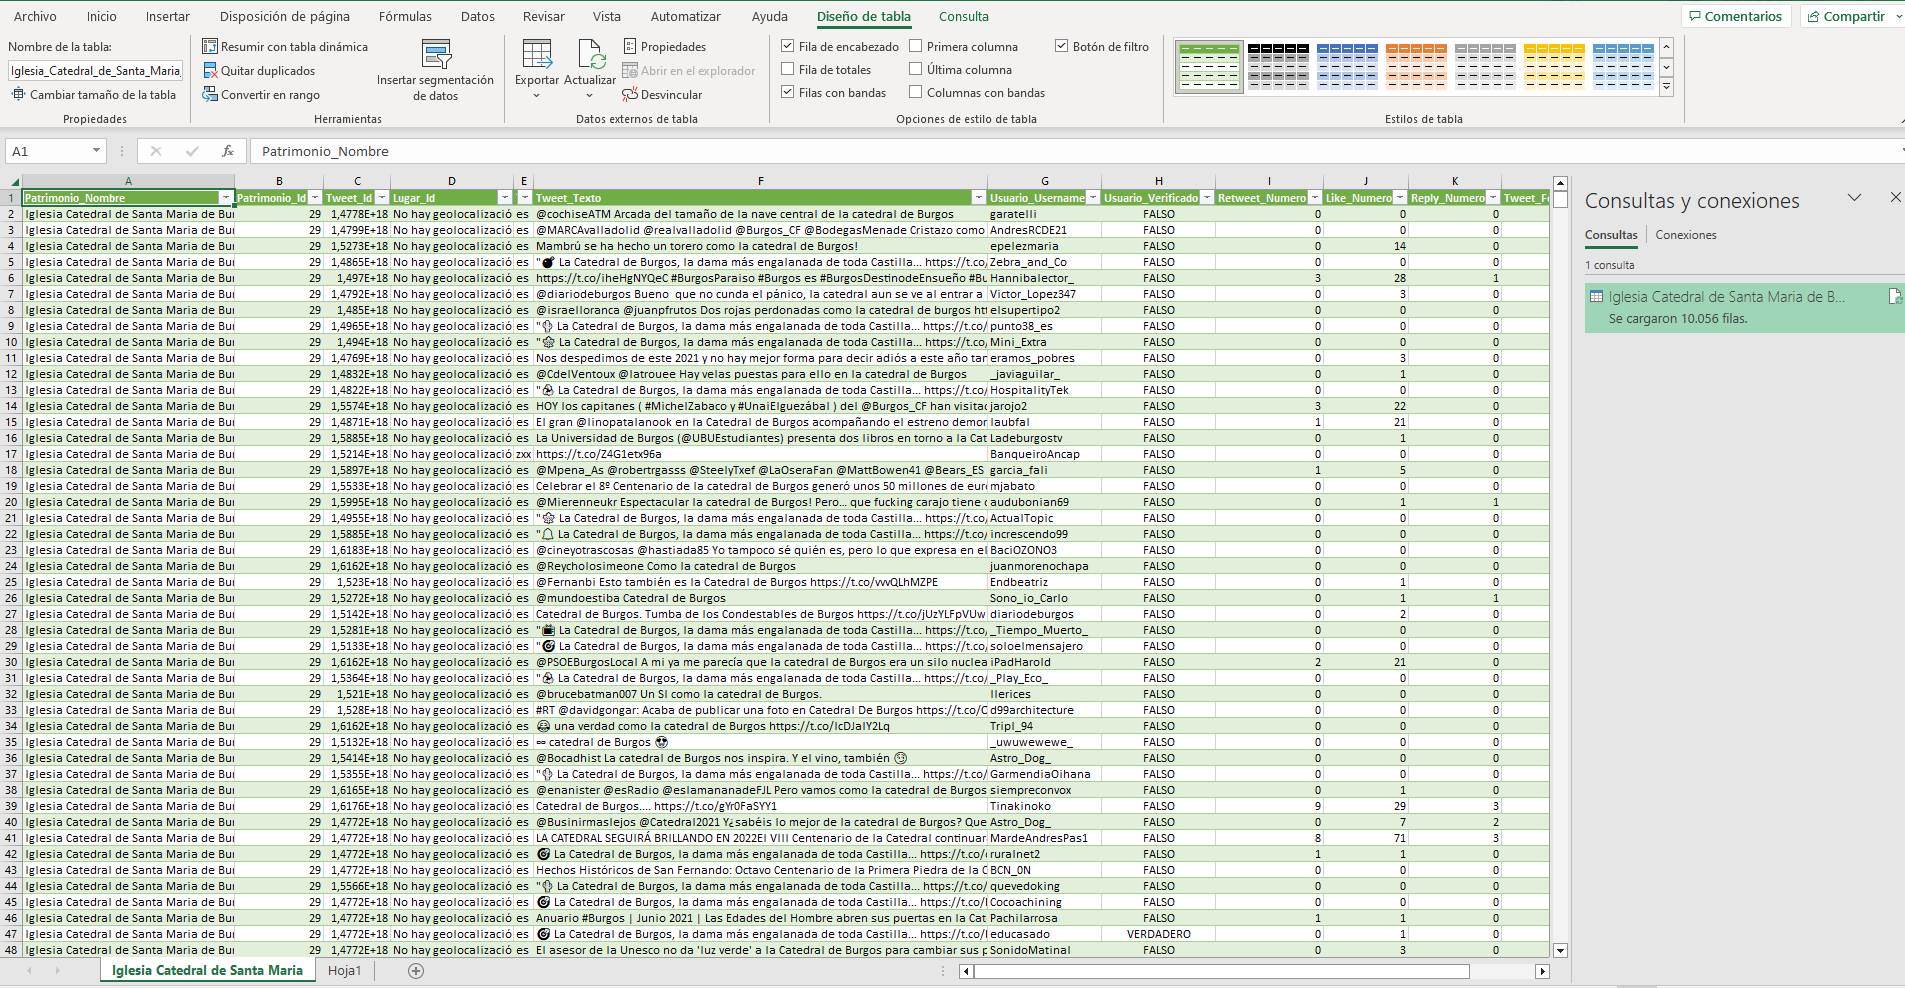
\includegraphics[scale=0.2]{img/Excel.png} \\
    \caption{Documentación de usuario - Visualización en Excel}
    \label{Documentación de usuario - Visualización en Excel}
\end{figure}
\subsection{Página de estadísticas temporales}
Una vez se ha pulsado en la barra navegadora el botón 'Estadísticas generales', se redireccionará al usuario a la página de estadísticas generales, en la que se mostrarán el total de tweets de todos los BIC entre las fechas existentes en la base de datos (Figura E.15).\\
Esta página permite modificar las fechas de inicio y fin de las estadísticas, teniendo en cuenta que la fecha de inicio debe ser anterior que la fecha de fin.
Además esta página permite volver a la página de inicio.
\begin{figure}[h!]
    \centering
    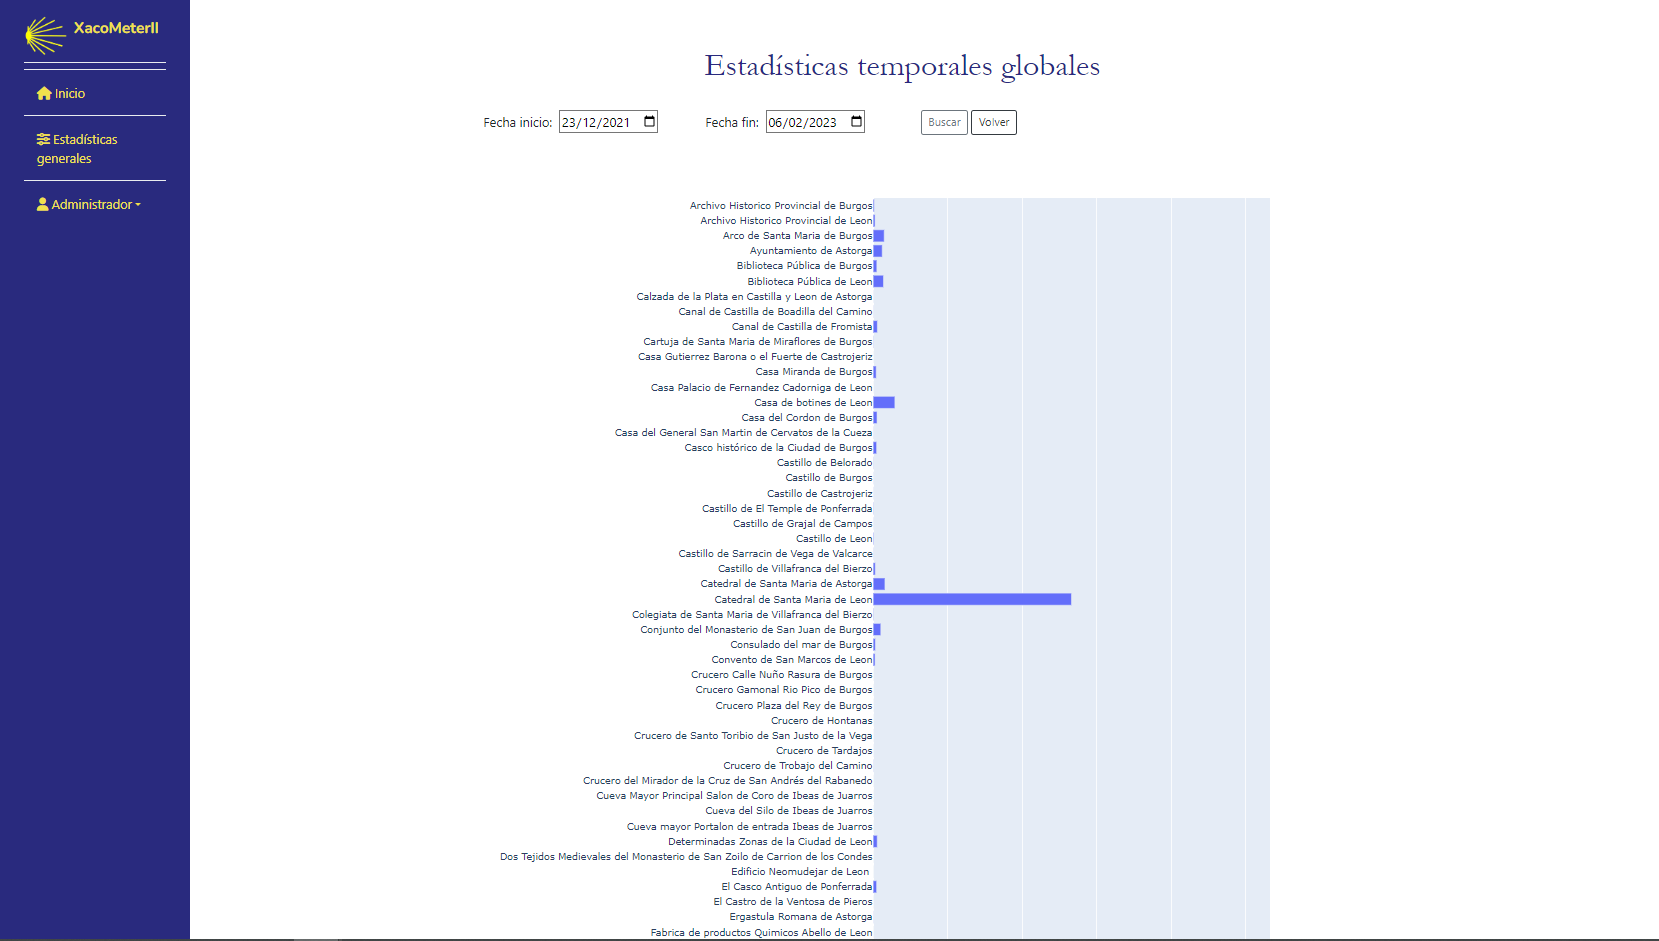
\includegraphics[scale=0.3]{img/EstadisticasGenerales.png} 
    \caption{Documentación de usuario - Estadísticas generales}
    \label{Documentación de usuario - Estadísticas generales}
\end{figure}
\subsection{Inicio de sesión}
Desde esta página se pueden introducir las credenciales de administrador (Figura E.16), que, si se introducen correctamente,  se continuará a las opciones del Administrador.
Estas credenciales son:
\begin{itemize}
    \item \textbf{USUARIO:} 'admin'
    \item \textbf{CONTRASEÑA:} 'Administrador1.'\\
\end{itemize}
\begin{figure}[h!]
    \centering
    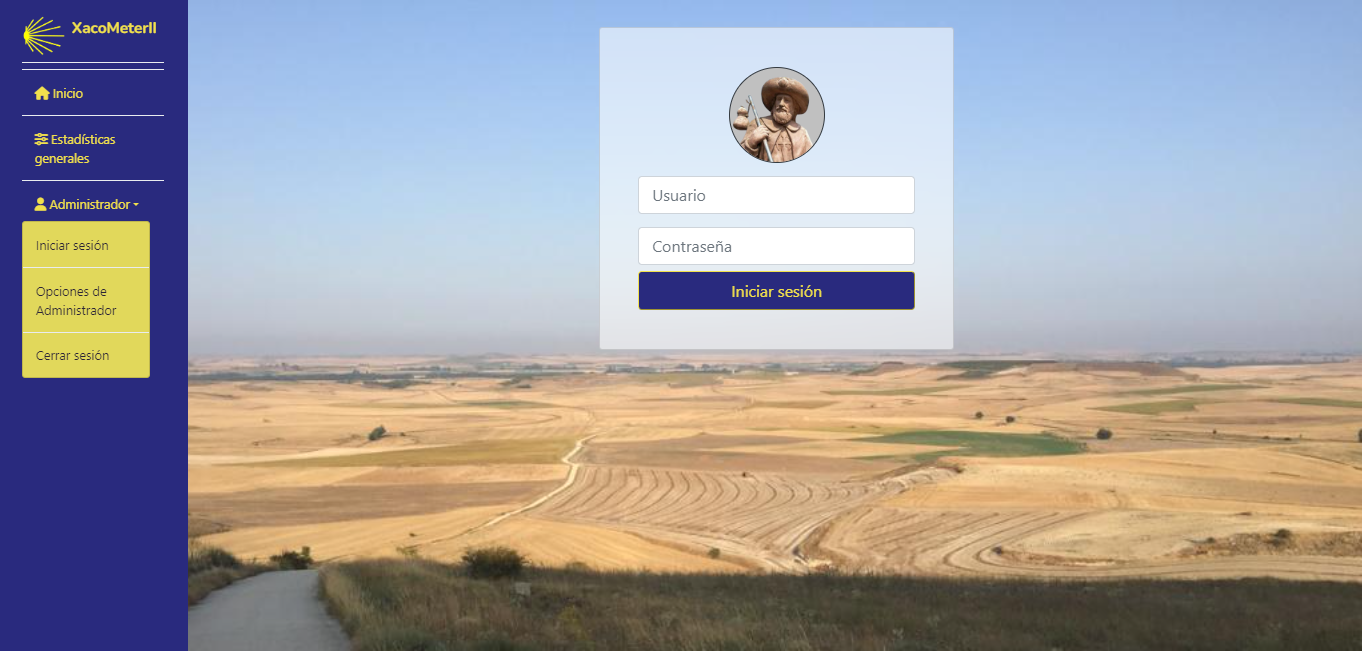
\includegraphics[scale=0.3]{img/Login.png} \\
    \caption{Documentación de usuario - Inicio de sesión}
    \label{Documentación de usuario - Inicio de sesión}
\end{figure}

\subsection{Opciones del administrador}
El administrador tiene tres opciones (Figura E.17):
\begin{enumerate}
    \item Crear una base de datos desde una fecha.
    \item Actualizar la base de datos desde la última fecha registrada hasta el día de hoy.
    \item Cerrar la sesión.
\end{enumerate}
Para acceder a cualquiera de estas tres opciones, se debe seleccionar sobre uno de los botones de esta página.
\begin{figure}[h!]
    \centering
    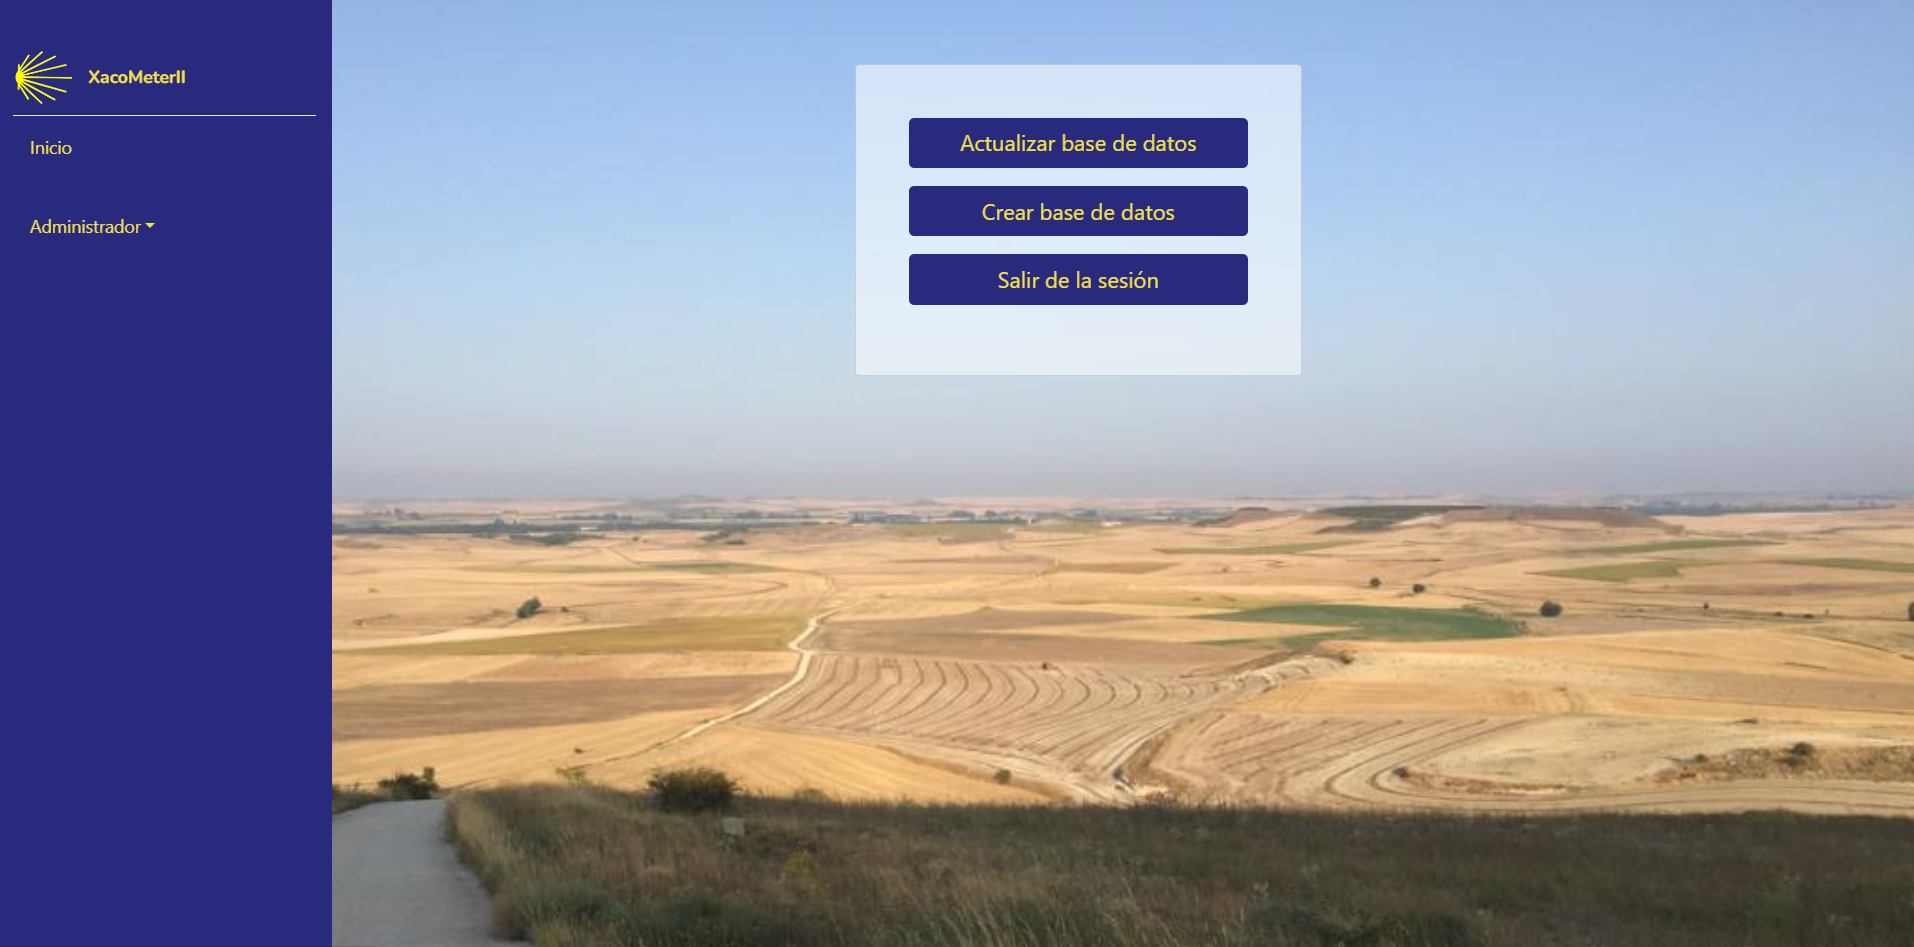
\includegraphics[scale=0.2]{img/OpcionesAdministrador.png} \\
    \caption{Documentación de usuario - Opciones del administrador}
    \label{Documentación de usuario - Opciones del administrador}
\end{figure}
\subsubsection{Creación de la base de datos}
En el caso de ser administrador y querer crear una base de datos, se requerirán unos parámetros para realizar las búsquedas (Figura E.18). Estos son las fechas que se quieren consultar y otros parámetros establecidos por Twitter que limitan nuestra búsqueda:
\begin{enumerate}
     \item Introducir las consultas que se van a realizar. Actualmente solo se pueden realizar máximo 300 consultas cada 15 minutos.
    \item El tiempo de duración de cada petición. Actualmente cada petición debe durar mínimo 1 segundo.
    \item El tiempo de espera entre las consultas especificadas en el primer parámetro y las siguientes consultas. Twitter ha definido que se podrán realizar máximo 300 consultas cada 15 minutos, por lo que se recomienda esperar 10 minutos, es decir, 600 segundos:\\
    $$ 15\hspace{0.5em}minutos\times60\frac{\text{segundos}}{\text{minuto}}=900\hspace{0.5em}segundos $$
    $$ 300\hspace{0.5em}peticiones\times1\frac{\text{segundo}}{\text{petición}}=300\hspace{0.5em}segundos $$
    $$ 900\hspace{0.5em}segundos\hspace{0.5em}-\hspace{0.5em} 300\hspace{0.5em}segundos\hspace{0.5em}=\hspace{0.5em}600\hspace{0.5em}segundos$$
\end{enumerate}
\begin{figure}[h!]
    \centering
    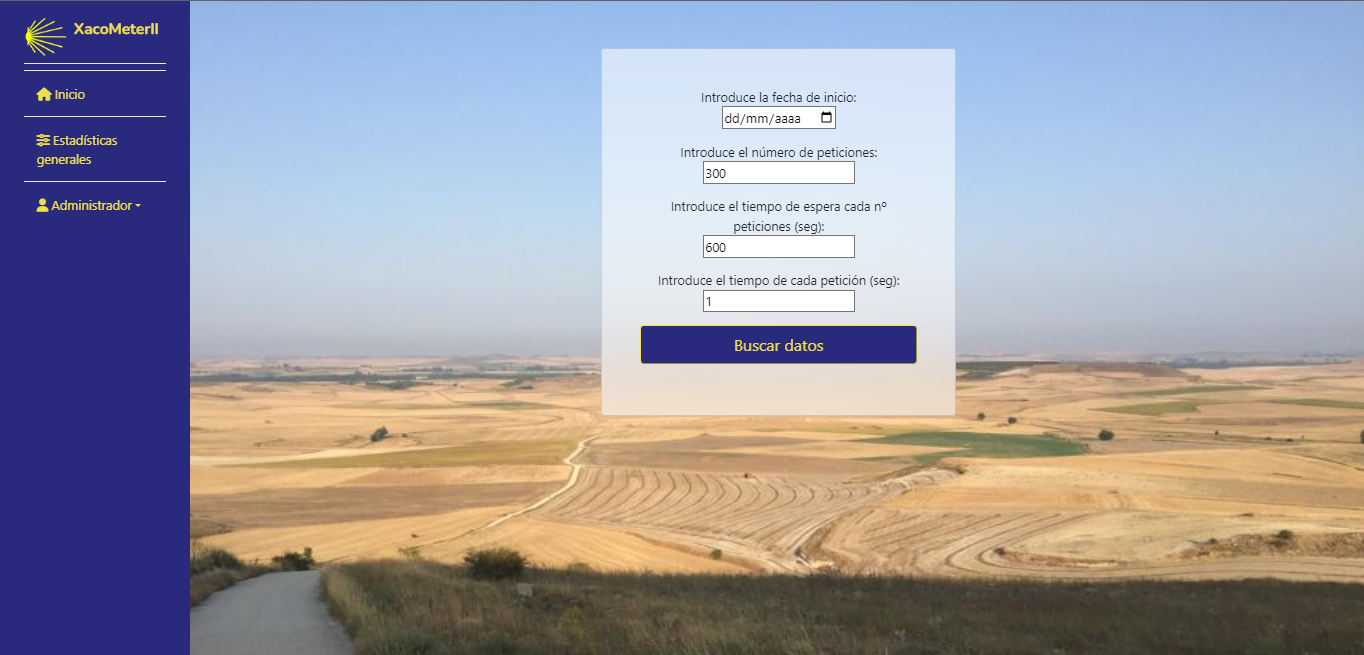
\includegraphics[scale=0.4]{img/CrearBD.png} \\
    \caption{Documentación de usuario - Crear base de datos}
    \label{Documentación de usuario - Crear base de datos}
\end{figure}
\subsection{Actualización de la base de datos}
Al igual que en el caso de 'Creación de la base de datos', se puede actualizar la base de datos marcando la fecha automáticamente, dándole el último valor de fecha almacenado en la base de datos. El usuario debe introducir los parámetros en base a las restricciones de Twitter (Figura E.19):\\
\begin{enumerate}
     \item Introducir las consultas que se van a realizar. Actualmente solo se podrán realizar máximo 300 consultas cada 15 minutos.
    \item El tiempo de duración de cada petición. Actualmente cada petición debe durar mínimo 1 segundo.
    \item El tiempo de espera entre las consultas especificadas en el primer parámetro y las siguientes consultas. Twitter ha definido que se podrán realizar máximo 300 consultas cada 15 minutos, por lo que se recomienda esperar 10 minutos, es decir, 600 segundos:\\
    $$ 15\hspace{0.5em}minutos\times60\frac{\text{segundos}}{\text{minuto}}=900\hspace{0.5em}segundos $$
    $$ 300\hspace{0.5em}peticiones\times1\frac{\text{segundo}}{\text{petición}}=300\hspace{0.5em}segundos $$
    $$ 900\hspace{0.5em}segundos\hspace{0.5em}-\hspace{0.5em} 300\hspace{0.5em}segundos\hspace{0.5em}=\hspace{0.5em}600\hspace{0.5em}segundos$$
\end{enumerate}
\begin{figure}[h!]
    \centering
    \includegraphics[scale=0.4]{img/ActualizarBD.png} \\
    \caption{Documentación de usuario - Actualizar base de datos}
    \label{Documentación de usuario - Actualizar base de datos}
\end{figure}
\subsection{Cerrar sesión}
En el caso de estar iniciada la sesión de 'Administrador', se puede salir de la sesión pulsando el botón \textbf{'Cerrar sesión'} (Figura E.20).\\
La sesión dura abierta 30 minutos, por lo que en el caso de querer continuar en la sesión se requerirá volver a introducir las credenciales.
\begin{figure}[h!]
    \centering
    \includegraphics[scale=0.75]{img/CerrarSesion.png} \\
    \caption{Documentación de usuario - Cierre de sesión}
    \label{Documentación de usuario - Cierre de sesión}
\end{figure}




\bibliographystyle{plain}
\bibliography{bibliografiaAnexos}

\end{document}
